\documentclass[
% a4paper, fontsize=10pt, BCOR=5mm, % reviewed version
  paper=6.69in:9.61in, fontsize=10pt, BCOR=9mm, DIV=15,
  pagesize=pdftex,
  headings=openright,
  headsepline,
  chapterprefix,
  appendixprefix,
  draft=false,
  listof=totoc,
  listof=leveldown
]{scrbook}

\usepackage[utf8]{inputenc}
\usepackage{graphicx}
\usepackage{csquotes}
\usepackage{booktabs}
\usepackage{listings}
\usepackage[ngerman,english]{babel}
\usepackage[hyphens]{url}
\PassOptionsToPackage{hyphens}{url}
\usepackage[hyperindex,breaklinks]{hyperref}
\usepackage{bookmark}
\usepackage{breakurl}
% textrightarrow U+2192
\usepackage{textcomp}
%\usepackage{enumitem}
%\setlist{nolistsep}
% algorithm
\usepackage{amsmath}
\usepackage{algorithm2e}


% for rotate tables
\usepackage{adjustbox}
\usepackage{pdflscape}
\usepackage{afterpage}

% \begin{Verbatim}[samepage=true]
\usepackage{fancyvrb}

\title{Measuring Metadata Quality}
\author{Péter Király}

% defining \chapterautor
\newcommand{\chapterauthor}[1]{%
  {\parindent0pt\vspace*{0pt}%
  \linespread{1.1}\large\scshape#1%
  \par\nobreak\vspace*{35pt}}
}

% show "Appendix" before appendices
\usepackage{xpatch}
\xapptocmd{\appendix}{%
  \addtocontents{toc}{%
    \RedeclareSectionCommand[
      tocdynnumwidth,
      tocentrynumberformat=\tocappendixnumber
    ]{chapter}%
  }%
}{}{\PatchFailed}
\newcommand\tocappendixnumber[1]{\chapapp~#1}

% JSON highlight
\usepackage{xcolor}
\colorlet{punct}{red!60!black}
\definecolor{background}{HTML}{EEEEEE}
\definecolor{delim}{RGB}{20,105,176}
\colorlet{numb}{magenta!60!black}

% numbers=left,
% numberstyle=\scriptsize,
% stepnumber=1,
% numbersep=8pt,
% backgroundcolor=\color{background},
% frame=lines,
%     literate=
%      *{0}{{{\color{numb}0}}}{1}
%       {1}{{{\color{numb}1}}}{1}
%       {2}{{{\color{numb}2}}}{1}
%       {3}{{{\color{numb}3}}}{1}
%       {4}{{{\color{numb}4}}}{1}
%       {5}{{{\color{numb}5}}}{1}
%       {6}{{{\color{numb}6}}}{1}
%       {7}{{{\color{numb}7}}}{1}
%       {8}{{{\color{numb}8}}}{1}
%       {9}{{{\color{numb}9}}}{1}
%       {:}{{{\color{punct}{:}}}}{1}
%       {,}{{{\color{punct}{,}}}}{1}
%       {\{}{{{\color{delim}{\{}}}}{1}
%       {\}}{{{\color{delim}{\}}}}}{1}
%       {[}{{{\color{delim}{[}}}}{1}
%       {]}{{{\color{delim}{]}}}}{1},

\lstdefinelanguage{json}{
    basicstyle=\normalfont\ttfamily,
    showstringspaces=false,
    breaklines=true,
}
% \title{Measuring Metadata Quality}
\author{Péter Király}
%\date{April 2019}
%\degreemonth{April}
%\university{Göttingen}

% \usepackage[natbib]{biblatex}
% \addbibresource{bibliography-for-papers.bib}

\begin{document}

% \maketitle
%\renewcommand{\thepage}{\roman{page}}

\frontmatter

\makeatletter

\begin{titlepage}
  \thispagestyle{empty}
  \begin{center}

  {\bfseries{\Huge\strut\@title\par}}
  \vspace{24pt}
  Thesis\\
in order to acquire the Doctoral Degree in Philosophy\\
at the Faculty of Humanities of the Georg-August-Universität Göttingen\\
  \vspace{24pt}
  submitted by\\
  \@author \\ from Debrecen\\
  \vspace{12pt}
  Göttingen 2019
  \end{center}
\end{titlepage}

\makeatother
%\input{titlepage}
\chapter*{Abstract}
\addcontentsline{toc}{chapter}{Abstract}

In the last 15 years different aspects of  metadata quality have been investigated. Researchers measured the established metrics on a variety of metadata collections. One common aspect of the majority of these research projects is that the tools they produce as a necessary side effect were not intended to be reused in other projects. This research, while focusing mainly on a specific metadata collection, Europeana, investigates  practical aspects of metadata quality measurement such as reusability, reproducability, scalability and adaptability.

Europeana.eu -- the European digital platform for cultural heritage -- aggregates metadata describing 58 million cultural heritage objects from more than 3200 libraries, museums, archives and audiovisual archives across Europe. The collection is heterogeneous with objects in different formats and languages and descriptions that are formed by different indexing practices. Often these records are also taken from their original context. In order to develop effective services for accessing and using the data we should know their strengths and weaknesses or in other words the quality of these data. The need for metadata quality is particularly motivated by its impact on user experience, information retrieval and data re-use in other contexts. In Chapter 2 the author proposes a method and an open source implementation to measure some structural features of these data, such as completeness, multilinguality and uniqueness. The investigation and exposure of record patterns is another aspect to reveal quality issues.

One of the key goals of Europeana is to enable users to retrieve cultural heritage resources irrespective of their origin and the material’s metadata language. The presence of multilingual metadata descriptions is therefore essential for successful cross-language retrieval. Quantitatively determining Europeana’s crosslingual reach is a prerequisite for enhancing the quality of metadata in various languages. Capturing multilingual aspects of the data requires us to take data aggregation lifecycle into account including data enhancement processes such as automatic data enrichment. In Chapter 3 the author presents an approach developed together with some members of Europeana Data Quality Committee for assessing multilinguality as part of data quality dimensions, namely completeness, consistency, conformity and accessibility. The chapter describes the defined and implemented measures, and provides initial results and recommendations.

The next chapter (Chapter 4) -- investigating the applicability of the above mentioned approach -- describes the method and results of validation of 16 library catalogues. The format of the catalog record is Machine Readable Cataloging (MARC21) which is the most popular metadata standard for describing books. The research investigates the structural features of the record and as a result finds and classifies different commonly found issues. The most frequent issues are usage of undocumented schema elements, improper values instead of using terms from controlled vocabulary, or the failure to meet other strict requirements.

The next chapters describe the engineering aspects of the research. First (Chapter 5), a short account of the structure of an extensible metadata quality assessment framework is given, which supports multiple metadata schemas, and is flexible enough to work with new schemas. The software has to be scalable to be able to process huge amount of metadata records within a reasonable time. Fundamental requirements that need to be considered during the design of such a software are i) the abstraction of the metadata schema (in the context of the measurement process), ii) how to address distinct parts within metadata records, iii) the workflow of the measurement, iv) a common and powerful interface for the individual metrics, and v) interoperability with Java and REST APIs. Second (Chapter 6), is an investigation of the optimal parameter settings for a long running, standalone mode Apache Spark based, stateless process. It measures the effects of four different parameters and compares the application's behaviour in two different servers. The most important lessons learned in this experiment is that allocating more resources does not necessary imply better performance. Moreover, what we really need in an environment with limited and shared resources is a `good enough' state which respectfully let other processes run. To find the optimal settings, it is suggested to pick up a smaller sample, which is similar to the full dataset in important features, and measure performance with different settings. The settings worth to check are number of cores, memory allocation, compression of the source files, and reading from different file systems (if they are available). As a source of ground truth Spark's default log, Spark event log, or measuring points inside the application can be used.

The final chapter explains future plans, the applicability of the method to other subdomains, such as Wikicite (the open citation data collection of Wikidata) and research data, and research collaborations with different cultural heritage institutions.



\begin{otherlanguage}{ngerman}
\chapter*{Zusammenfassung}
\addcontentsline{toc}{chapter}{Zusammenfassung}

\chapterauthor{Übersetzt von Juliane Stiller}

In den letzten 15 Jahren wurden verschiedene Aspekte von Metadatenqualität untersucht. In verschiedenen Metadatenkollektionen haben Wissenschaftler und Wissenschaftlerinnen Messwerte für etablierte Kennzahlen erfasst. Gemeinsam ist diesen Forschungsprojekten, dass die für die Messungen benötigten Werkzeuge häufig nicht darauf ausgelegt sind in anderen Projekten wiederverwendet zu werden. Die vorliegende Arbeit beschäftigt sich hauptsächlich mit der speziellen Metadatenkollektion von Europeana und untersucht dabei die praktischen Aspekte von Kriterien zur Messung von Metadatenqualität, wie Wiederverwendung, Reproduzierbarkeit, Skalierbarkeit und Anpassungsfähigkeit.

Europeana.eu, die europäische digitale Plattform für kulturelles Erbe, sammelt Metadaten von 58 Millionen kulturellen Objekten, die aus mehr als 3200 Bibliotheken, Museen, Archiven und audiovisuellen Archiven in Europa stammen. Diese Sammlung ist heterogen und besteht aus Objekten in verschiedenen Formaten und Sprachen, deren Beschreibungen durch unterschiedliche Indexierungspraktiken entstanden sind. Oft wurden die Objekte aus ihrem ursprünglichen Kontext genommen. Um nun Dienstleistungen zu entwickeln, mit denen die Daten zugänglich gemacht und genutzt werden können, muss man die Stärken und Schwächen oder anders ausgedrückt die Qualität der Daten kennen. Der Bedarf an qualitativ hochwertigen Daten ist durch deren Einfluss auf die Nutzererfahrung, das Information Retrieval und die Wiederverwendung von Daten in anderen Zusammenhängen motiviert. Im zweiten Kapitel schlägt der Autor eine Methode sowie eine Open Source Lösung vor, um strukturelle Eigenschaften von Daten, wie Vollständigkeit, Multilingualität und Eindeutigkeit, zu messen. Eine weitere Komponente, um Probleme in Daten aufzudecken, ist die Analyse und Veranschaulichung von Dokumentstrukturen.

Ein zentrales Anliegen von Europeana ist es, Nutzern und Nutzerinnen die Möglichkeit zu bieten Kulturgüter unabhängig ihrer Herkunft und Sprache, in der sie beschrieben sind, zu finden. Für ein erfolgreiches sprachübergreifendes Retrieval sind mehrsprachige Metadatenbeschreibungen unerlässlich. Eine Voraussetzung um überhaupt die Metadatenqualität in verschiedenen Sprachen verbessern zu können, ist die quantitative Bestimmung der sprachlichen Vielfalt der Metadaten in Europeana. Um die Mehrsprachigkeit in den Daten erfassen zu können, müssen der komplette Prozess der Datenaggregation abgebildet und auch Prozesse zur Datenverbesserung, wie beispielsweise automatische Datenanreicherungen, berücksichtigt werden. In Kapitel 3 präsentiert der Autor eine Methode, die er zusammen mit Mitgliedern des Europeana Data Quality Committees entwickelt hat, um Mehrsprachigkeit als Aspekt verschiedener Dimensionen von Datenqualität, wie Vollständigkeit, Konsistenz, Konformität und Zugänglichkeit, messen zu können.

Das nächste Kapitel (Kapitel 4) geht darauf ein, wie der oben beschriebene Prozess umgesetzt werden kann und beschreibt die dahingehende Methode und die Ergebnisse ihrer Validierung mit 16 Bibliothekskatalogen. Die Katalogsdatei liegt im Machine Readable Cataloging (MARC21)-Format vor, dem am weitesten verbreiteten Metadatenstandard zur Beschreibung von Büchern. Die Forschung untersucht die strukturellen Merkmale der Daten auf deren Basis häufig auftretende Probleme gefunden und klassifiziert werden. Die häufigsten Probleme sind die Verwendung von undokumentierten Schema-Elementen, falsche Werte an Stellen, an denen ein Wert aus einem kontrollierten Vokabular? hätte übernommen werden sollen oder andere strenge Anforderungen erfüllt werden müssen.

Das nächste Kapitel (Kapitel 4) geht darauf ein, wie das oben beschriebene Konzept skalierbar umgesetzt werden kann und beschreibt die Methode und die Ergebnisse der Validierung von 16 Bibliothekskatalogen. Die Katalogdatensätze liegen in einem maschinenlesbaren Format  (MARC21) vor, dem am weitesten verbreiteten Metadatenstandard zur Beschreibung von bibliographischen Einheiten. Die vorliegende Untersuchung ermittelt strukturelle Merkmale der Datensätze und klassifiziert die in diesen häufig auftretenden Probleme. Die häufigsten Probleme sind die Verwendung von undokumentierten Schema-Elementen, falsche Werte an Stellen, an denen ein Wert aus einem kontrollierten Vokabular hätte übernommen werden sollen oder die Missachtung anderer strenger Vorgaben.

Die nächsten Kapitel beschreiben die technischen Aspekte der Forschung. In Kapitel 5 wird ein kurzer Überblick über den Aufbau des erweiterbaren Framework zur Messung von Metadatenqualität gegeben. Dieser unterstützt verschiedene Metadatenschemata und ist flexibel genug, um mit neuen Schemata umgehen zu können. Diese Anwendung muss skalierbar sein, um eine große Anzahl von Metadatensätzen innerhalb einer angemessenen Zeit verarbeiten zu können. Grundlegende Anforderungen, die bei der Entwicklung einer solchen Software berücksichtigt werden müssen, sind i) die Abstraktion des Metadatenschemas (im Rahmen des Messprozesses), ii) der Umgang mit unterschiedlichen Teilen innerhalb von Metadatensätzen, iii) der Messprozess, iv) eine gemeinsame und leistungsfähige Schnittstelle für die einzelnen Metriken und v) die Interoperabilität mit Java- und REST-APIs. In Kapitel 6 wird untersucht welche optimalen Parametereinstellungen für einen lang laufenden Prozess, basierend auf dem Apache Spark Stand-Alone-Modus, nötig sind. Dafür werden die Auswirkungen von vier verschiedenen Parametern gemessen und das Verhalten der Anwendung auf zwei verschiedenen Servern verglichen. Die wichtigste Erkenntnis aus diesem Experiment ist, dass die Zuweisung von mehr Ressourcen nicht unbedingt eine bessere Leistung bedeutet. In einem Umfeld mit begrenzten und geteilten Ressourcen brauchen wir einen Zustand, der "gut genug" ist und anderen Prozessen den Vortritt lässt. Um die optimalen Einstellungen zu finden und die Performance mit verschiedenen Parametern zu messen, sollte ein kleineres Sample herangezogen werden, das in wichtigen Merkmalen dem vollständigen Datensatz ähnelt. Die Einstellungen, die überprüft werden sollten, sind die Anzahl der Rechenkerne, die Speicherzuweisung, die Kompression der Quelldateien und (falls vorhanden) das Auslesen verschiedener Dateisysteme. Als Grundlage der Bewertung können das Standard-Spark-Logging sowie das Event-Logging oder Messpunkte innerhalb der Anwendung verwendet werden.

Das letzte Kapitel (Kapitel 7) erläutert Zukunftspläne, die Anwendbarkeit der Methode auf andere Bereiche wie Wikicite (die offene Datenbank für Zitationsdaten von Wikidata) und Forschungsdaten, sowie Forschungskooperationen mit verschiedenen Kulturerbeinstitutionen.
\end{otherlanguage}

\pdfbookmark[0]{Contents}{toc}
\tableofcontents



\mainmatter

\chapter{Introduction}

In the cultural heritage section there is a long tradition of building catalogues. During the centuries museums, archives and libraries developed different systems to record their collections.

There is no good definition for the quality, but much of the literature agrees that quality should somehow be in line with the `fitness for purpose', i.e. the quality of an object should be measured as how much the object supports a given purpose. The main purposes of the cultural heritage metadata are registering the collection and helping users in discovery. The functional analysis of MARC 21 format (the most popular metadata  schema for bibliographic records) goes further and sets up functional groups, such as search, identity, select, manage, process and classifies the underlying schema elements to these categories~\cite{frbr1998, delsey2003, loc2006}. So by analysing the fields of the individual records, we can more precisely tell which aspects of the quality are good or bad.

These records are not only for registration and helping discovery of the materials, they are also the sources of additional researches in the Humanities. The catalogue contains lots of factual information, which are not available in other sources (or not in organised way), and therefore before the age of digitisation one could have found the printed catalogues of the most important collections (e.g. British Library, Library of Congress etc.) in the reading rooms of research institutions. In the past two decades several research projects attached existing library metadata to different types of full text datasets (optical character recognised or XML encoded versions), to provide additional facets for the analysis process such as personal or institutional names (creators, publishers), geographical information (places of publication), time span and so on.

Just a few examples: KOLIMO (Corpus of Literary Modernism)\footnote{\url{https://kolimo.uni-goettingen.de/index.html}} uses TEI headers containing catalogue information as well as other metadata, for extracting literature and language features specific to a given time period, or to a particular author. OmniArt~\cite{strezoski2017} is a research project, based on the metadata of Rijksmuseum (Amsterdam), the Metropolitan Museum of Arts (New York) and the Web Gallery of Art\footnote{\url{https://www.wga.hu/}}. They collected 432,217 digital images with curated metadata (which is the largest collection of that kind) to run categorical analysis. Benjamin Schmidt uses the HathiTrust\footnote{\url{https://www.hathitrust.org/}} digital library and its metadata records to test machine learning classification algorithms, where he can compare the results with the Library of Congress subject headings available in the metadata records~\cite{smith2017}. The common features of these project is that they use cultural heritage institutions’ catalogue data as primary sources in their own research. It is self evident, that quality of those data might have effect on the conclusions of the research, and on the other hand it is beyond the responsibilities and possibilities of a researcher (or even a research group) to validate the records one by one, and fix them as needed.

This third use case of cultural heritage data become so frequent recently, that two years ago it lead to coining a new phrase: ``collections as data''. As the Santa Barbara Statement on Collections as Data~\cite{santabarbarastatement2017} summarises: ``For decades, cultural heritage institutions have been building digital collections. Simultaneously, researchers have drawn upon computational means to ask questions and look for patterns. This work goes under a wide variety of names including but not limited to text mining, data visualisation, mapping, image analysis, audio analysis, and network analysis. With notable exceptions [...], cultural heritage institutions have rarely built digital collections or designed access with the aim to support computational use. Thinking about collections as data signals an intention to change that.'' While collections as data movement emphasises the importance of re-usability of cultural heritage data, and we expect that this great and important movement will help organisations to think more about the scientific usage or their metadata,\footnote{A 2016 report which analyses the usage of two important British cultural heritage collections mentions that ``The citation evidence that is available shows a growing literature that mentions using EEBO [Early English Books Online] or HCPP [House of Commons Parliamentary Papers]'', and ``Shifts to humanities data science and data-driven research are of growing interest to scholars''.~\cite{meyer2016}} their principles are focusing on access, and get rid of current barriers, however misses the aspects of quality. The quality assessment aspect we propose in this project would be a complementary element next to the other principles.

%%%
\section{Metadata quality}

\quote{``We know it [i.e. metadata quality] when we see it, but conveying the full bundle of assumptions and experience that allow us to identify it is a different matter.'' (Bruce and Hillmann)~\cite{bruce-hillmann2004}.}

The (US) National Information Standards Organization (NISO) provides a definition for metadata, which is ``structured information that describes, explains, locates, or otherwise represents something else.''~\cite{framework2007} The interesting thing in this definition is the list of verbs: describes, explains, locates, and represents. Metadata is not a static entity, it has multiple different functions and should be in context of other entities. That is in harmony with the famous the quality assurance slogan `fitness for purpose'. There are different definitions of the slogan, some of them are

\begin{itemize}
 \setlength{\parskip}{0pt}
 \setlength{\itemsep}{0pt plus 1pt}
 \item fulfilment of a specification or stated outcomes
 \item measured against what is seen to be the goal of the unit
 \item achieving institutional mission and objectives
\end{itemize}

From these definitions we can draw two important conclusions:

1) an object's quality is not an absolute value, it depends on the context of the object, what goal(s) the agents in the current context would like to achieve with the help of the object

2) the quality is a multi-faceted value. As the object might have different functions, we should evaluate the fulfilment's of them independently.

NISO's definition of metadata nicely fits into this framework, as it highlights the multi-faceted and contextual nature of metadata.

In an aggregated metadata collection such as Europeana, the main purpose of the metadata is to provide access points to the objects which the metadata describe (and stored remotely in the providing cultural heritage institutions, outside of Europeana). If the metadata stored in Europeana is of low quality or missing, the service will not be able to provide access points, and the user will not use the object.

% more explanation:
% Data on the Web Best Practices
% W3C Working Draft, https://www.w3.org/TR/dwbp/

As Bruce and Hillmann states, an expert could recognise if a given metadata record is ``good'' or ``bad''. What we would like to achieve is to formalise this knowledge by setting up the dimensions of the quality, and establishing metrics and measurement methods.

\section{Metrics in the literature}

In the literature of metadata quality assessment (see Appendix A) one can find a number of metric definitions. In this section I review some of them which proved to be relevant in my research.

Regarding to the cultural heritage context Bruce and Hillmann's above cited seminal paper (\cite{bruce-hillmann2004}) defines the data quality metrics. Palavitsinis in his PhD thesis \cite{palavitsinis2014} summarises them as follows:

\emph{Completeness}: Number of metadata elements filled out by the annotator in comparison to the total number of elements in the application profile

\emph{Accuracy}: In an accurate metadata record, the data contained in the fields, correspond to the resource that is being described

\emph{Consistency}: Consistency measures the degree to which the metadata values provided are compliant to what is defined by the metadata application profile

\emph{Objectiveness}: Degree in which the metadata values provided, describe the resource in an unbiased way, without undermining or promoting the resource

\emph{Appropriateness}: Degree to which the metadata values provided are facilitating the deployment of search mechanisms on top of the repositories

\emph{Correctness}: The degree to which the language used in the metadata is syntactically and grammatically correct

The same author -- analysing the metadata quality literature focusing mainly on the Learning Object Repositories metadata -- lists the following additional dimensions proposed by different authors: accessibility, conformance, currency, intelligibility, objectiveness, presentation, provenance, relevancy and timeliness. He also repeats the categorisation of Lee et al. \cite{lee2002} regarding to the quality dimensions:

Intrinsic Metadata Quality: represents dimensions that recognise that metadata may have innate correctness regardless of the context in which it is being used. For example, metadata for a digital object may be more or less ‘accurate’ or ‘unbiased’ in its own right,

Contextual Metadata Quality: recognises that perceived quality may vary according to the particular task at hand, and that quality must be relevant, timely, complete, and appropriate in terms of amount, so as to add value to the purpose for which the information will be used,

Representational Metadata Quality: addresses the degree to which the metadata being assessed is easy to understand and is presented in a clear manner that is concise and consistent,

Accessibility Metadata Quality: references the ease with which the metadata is obtained, including the availability of the metadata and timeliness of its receipt.

Zaveri Amrapali and her colleagues surveyed the Linked Data Quality literature in 2015~\cite{zaveri2015}. Their work became the most cited paper regarding to data quality. They investigated what quality dimensions and metrics were suggested by other authors and grouped individual metrics into the following dimensions:

\emph{Accessibility dimensions}

Availability -- the extent to which data (or some portion of it) is present, obtainable, and ready for use. The metrics this dimension are:
\begin{itemize}
 \setlength{\parskip}{0pt}
 \setlength{\itemsep}{0pt plus 1pt}
 \item A1 accessibility of the SPARQL endpoint and the server
 \item A2 accessibility of the RDF dumps
 \item A3 dereferenceability of the URI
 \item A4 no misreported content types
 \item A5 dereferenced forward-links
\end{itemize}

Licensing -- the granting of permission for a customer to reuse a dataset under defined conditions.
\begin{itemize}
 \setlength{\parskip}{0pt}
 \setlength{\itemsep}{0pt plus 1pt}
 \item L1 machine-readable indication of a license
 \item L2 human-readable indication of a license
 \item L3 specifying the correct license
\end{itemize}

Interlinking -- the degree to which entities that represent the same concept are linked to each other, be it within or between two or more data sources.
\begin{itemize}
 \setlength{\parskip}{0pt}
 \setlength{\itemsep}{0pt plus 1pt}
 \item I1 detection of good quality interlinks
 \item I2 existence of links to external data providers
 \item I3 dereferenced back-links
\end{itemize}

Security -- the extent to which data is protected against alteration and misuse.
\begin{itemize}
 \setlength{\parskip}{0pt}
 \setlength{\itemsep}{0pt plus 1pt}
 \item S1 usage of digital signatures
 \item S2 authenticity of the dataset
\end{itemize}

Performance -- the efficiency of a system that binds to a large dataset.
\begin{itemize}
 \setlength{\parskip}{0pt}
 \setlength{\itemsep}{0pt plus 1pt}
 \item P1 usage of slash-URIs
 \item P2 low latency
 \item P3 high throughput
 \item P4 scalability of a data source
\end{itemize}

\emph{Intrinsic dimensions}

Syntactic validity -- the degree to which an RDF document conforms to the specification of the serialization format
\begin{itemize}
 \setlength{\parskip}{0pt}
 \setlength{\itemsep}{0pt plus 1pt}
 \item SV1 no syntax errors of the documents
 \item SV2 syntactically accurate values
 \item SV3 no malformed datatype literals
\end{itemize}

Semantic accuracy -- the degree to which data values correctly represent the real-world facts
\begin{itemize}
 \setlength{\parskip}{0pt}
 \setlength{\itemsep}{0pt plus 1pt}
 \item SA1 no outliers
 \item SA2 no inaccurate values
 \item SA3 no inaccurate annotations, labellings or classifications
 \item SA4 no misuse of properties
 \item SA5 detection of valid rules
\end{itemize}

Consistency -- a knowledge base is free of (logical/formal) contradictions with respect to particular knowledge representation and inference mechanisms
\begin{itemize}
 \setlength{\parskip}{0pt}
 \setlength{\itemsep}{0pt plus 1pt}
 \item CS1 no use of entities as members of disjoint classes
 \item CS2 no misplaced classes or properties
 \item CS3 no misuse of owl:DatatypeProperty or owl:ObjectProperty
 \item CS4 members of owl:DeprecatedClass or owl:DeprecatedProperty not used
 \item CS5 valid usage of inverse-functional properties
 \item CS6 absence of ontology hijacking
 \item CS7 no negative dependencies/correlation among properties
 \item CS8 no inconsistencies in spatial data
 \item CS9 correct domain and range definition
 \item CS10 no inconsistent values
\end{itemize}

Conciseness -- the minimization of redundancy of entities at the schema and the data level
\begin{itemize}
 \setlength{\parskip}{0pt}
 \setlength{\itemsep}{0pt plus 1pt}
 \item CN1 high intensional conciseness
 \item CN2 high extensional conciseness
 \item CN3 usage of unambiguous annotations/labels
\end{itemize}

Completeness -- the degree to which all required information is present in a particular dataset
\begin{itemize}
 \setlength{\parskip}{0pt}
 \setlength{\itemsep}{0pt plus 1pt}
 \item CM1 schema completeness
 \item CM2 property completeness
 \item CM3 population completeness
 \item CM4 interlinking completeness
\end{itemize}

\emph{Contextual dimensions}

Relevancy -- the provision of information which is in accordance with the task at hand and important to the users’ query
\begin{itemize}
 \setlength{\parskip}{0pt}
 \setlength{\itemsep}{0pt plus 1pt}
 \item R1 relevant terms within metainformation attributes
 \item R2 coverage
\end{itemize}

Trustworthiness -- the degree to which the information is accepted to be correct, true, real, and credible
\begin{itemize}
 \setlength{\parskip}{0pt}
 \setlength{\itemsep}{0pt plus 1pt}
 \item T1 trustworthiness of statements
 \item T2 trustworthiness through reasoning
 \item T3 trustworthiness of statements, datasets and rules
 \item T4 trustworthiness of a resource
 \item T5 trustworthiness of the information provider
 \item T6 trustworthiness of information provided (content trust)
 \item T7 reputation of the dataset
\end{itemize}

Understandability -- the ease with which data can be comprehended without ambiguity and be used by a human information consumer
\begin{itemize}
 \setlength{\parskip}{0pt}
 \setlength{\itemsep}{0pt plus 1pt}
 \item U1 human-readable labelling of classes, properties and entities as well as presence of metadata
 \item U2 indication of one or more exemplary URIs
 \item U3 indication of a regular expression that matches the URIs of a dataset
 \item U4 indication of an exemplary SPARQL query
 \item U5 indication of the vocabularies used in the dataset
 \item U6 provision of message boards and mailing lists
\end{itemize}

Timeliness -- how up-to-date data is relative to a specific task
\begin{itemize}
 \setlength{\parskip}{0pt}
 \setlength{\itemsep}{0pt plus 1pt}
 \item TI1 freshness of datasets based on currency and volatility
 \item TI2 freshness of datasets based on their data source
\end{itemize}

\emph{Representational dimensions}

Representational conciseness -- the representation of the data, which is compact and well formatted on the one hand and clear and complete on the other hand
\begin{itemize}
 \setlength{\parskip}{0pt}
 \setlength{\itemsep}{0pt plus 1pt}
 \item RC1 keeping URIs short
 \item RC2 no use of prolix RDF features
\end{itemize}

Interoperability -- the degree to which the format and structure of the information conform to previously returned information as well as data from other sources
\begin{itemize}
 \setlength{\parskip}{0pt}
 \setlength{\itemsep}{0pt plus 1pt}
 \item IO1 re-use of existing terms
 \item IO2 re-use of existing vocabularies
\end{itemize}

Interpretability -- technical aspects of the data, that is, whether information is represented using an appropriate notation and whether the machine is able to process the data
\begin{itemize}
 \setlength{\parskip}{0pt}
 \setlength{\itemsep}{0pt plus 1pt}
 \item IN1 use of self-descriptive formats
 \item IN2 detecting the interpretability of data
 \item IN3 invalid usage of undefined classes and properties
 \item IN4 no misinterpretation of missing values
\end{itemize}

Versatility -- the availability of the data in different representations and in an internationalized way
\vspace{0mm}
\begin{itemize}
 \setlength{\parskip}{0pt}
 \setlength{\itemsep}{0pt plus 1pt}
 \item V1 provision of the data in different serialization formats
 \item V2 provision of the data in various languages
\end{itemize}

Some of these metrics are relevant only in Linked Data context (those which are LD technology specific, such as SPARQL endpoint or RDF dump). On the other hand there are lots of metrics which are useful for non-linked metadata as well. For example we will see in Chapter 2 that there is a tendency to add misinterpretable ad-hoc values into a placeholder (``+++EMPTY+++'' to quote an extreme case) when the value is missing. `V2 provision of the data in various languages' is similar concept than the multilinguality I'll describe in Chapter 3. Downloadable dumps are also very useful even it is not in a specific (e.g. RDF) format.

\subsection{FAIR metrics}

One of the main recent developments regarding to research data management was the formulation of FAIR principles.~\cite{wilkinson2016}. ``The FAIR Principles provide guidelines for the publication of digital resources such as datasets, code, workflows, and research objects, in a manner that makes them Findable, Accessible, Interoperable, and Reusable.'' It became the starting point of many different projects which either implement the principles, or investigate further extensions. One of the is FAIRMetrics~\cite{wilkinson2018, fairmetrics}. It concentrates on the measurement aspects of the FAIR principles: how can we set up metrics upon which we can validate the ``fairness'' or research data.

The authors suggested, that good metrics in general should have the following properties:

\begin{itemize}
 \setlength{\parskip}{0pt}
 \setlength{\itemsep}{0pt plus 1pt}
 \item clear
 \item realistic
 \item discriminating
 \item measurable
 \item universal
\end{itemize}

There are 14 FAIR principles, and for each there is a metric. Each metric answers questions, such as `What is being measured?', `Why should we measure it?', `How do we measure it?', `What is a valid result?', `For which digital resource(s) is this relevant?' etc.

The creators published the individual metrics as nanopublications and they are working on an implementation. Besides the metrics they defined `Maturity Indicator tests' which are available as REST API backed by a Ruby based software called FAIR Evaluator. Maturity Indicators are an open set of metrics. Above the core set (which presented by the FAIRMetrics), the creators invited the research communities to create their own indicators. As they emphasise: ``we view FAIR as a continuum of `behaviors' exhibited by a data resource that increasingly enable machine discoverability and (re)use.''

The FAIRmetrics are as follows:

\begin{itemize}
 \setlength{\parskip}{0pt}
 \setlength{\itemsep}{0pt plus 1pt}
 \item F1: Identifier Uniqueness (Whether there is a scheme to uniquely identify the digital resource.)
 \item F1: Identifier persistence (Whether there is a policy that describes what the provider will do in the event an identifier scheme becomes deprecated.)
 \item F2: Machine-readability of metadata (The availability of machine-readable metadata that describes a digital resource.)
 \item F3: Resource Identifier in Metadata (Whether the metadata document contains the globally unique and persistent identifier for the digital resource.)
 \item F4: Indexed in a searchable resource (The degree to which the digital resource can be found using web-based search engines.)
 \item A1.1: Access Protocol (The nature and use limitations of the access protocol.)
 \item A1.2: Access authorization (Specification of a protocol to access restricted content.)
 \item A2: Metadata Longevity (The existence of metadata even in the absence/removal of data.)
 \item I1: Use a Knowledge Representation Language (Use of a formal, accessible, shared, and broadly applicable language for knowledge representation.)
 \item I2: Use FAIR Vocabularies (The metadata values and qualified relations should themselves be FAIR, for example, terms from open, community-accepted vocabularies published in an appropriate knowledge-exchange format.)
 \item I3: Use Qualified References (Relationships within (meta)data, and between local and third-party data, have explicit and `useful' semantic meaning)
 \item R1.1: Accessible Usage License (The existence of a license document, for both (independently) the data and its associated metadata, and the ability to retrieve those documents)
 \item R1.2: Detailed Provenance (There is provenance information associated with the data, covering at least two primary types of provenance information: -- Who/what/When produced the data (i.e. for citation); -- Why/How was the data produced (i.e. to understand context and relevance of the data))
 \item R1.3: Meets Community Standards (Certification, from a recognized body, of the resource meeting community standards.)
\end{itemize}

Most of these metrics rather measure the data repository, than individual research data sets. In this thesis I do not work with research data, it is among my future plans, but it is good to note that FAIRmetrics does not cover classical metadata quality metrics (such as completeness, accuracy etc.), so even if it will have a robust implementation, there will be space left for future research on research (meta)data quality, and on the other hand some of these metrics are applicable for cultural heritage data (e.g. persistent identifiers would help the ingestion process of Europeana, so the \emph{Identifier persistence} metric would be a useful indicator in this workflow).

\subsection{Vocabularies for validating Linked Data}

The domain of Linked Data (or semantic web) is based on `Open World assumption', which means that objects (entities) and statements about them are separated, different agents could create a statement about an object. Practically it means that there is no concept as ``record'', since the object does not have clear boundaries. The traditional record based systems have schemas, which describe what kind of statements could be done about an entity. For example the Dublin Core Metadata Element Set consists of 15 metadata element. If we would like to record a colour of a book in this schema, we can not do it directly. Of course we can put this information into a semantically more generic field, such as ``format'', but then we will loose specificity, and colour will be stored together with other features such as size, dimensions etc. In Linked Data context the situation is different: we can easily introduce a new property, and create a statement, however we loose the control of the schema. We can not tell if the new property is valid or not.

To solve this problem W3C set up RDF Data Shapes working group ``to produce a language for defining structural constraints on RDF graphs''\footnote{\url{https://www.w3.org/2014/data-shapes/charter}}. One of the results came from this approach is Shapes Constraint Language (SHACL)\footnote{\url{https://www.w3.org/TR/shacl/}. We should note that there is another approach for the same problem: Shape Expressions (ShEx) available at \url{http://shex.io}.}

SHACL defined a vocabulary (see Table \ref{table:shacl}) upon which one can create validation rules. It does not set metrics directly, but these constraint definitions are very useful building blocks of a data quality measurement system. The implementation of SHACL is based on Linked Data, but the definitions are meaningful in other contexts as well.

\begin{table}[ht]
\caption{Core constraints in SHACL}
\label{table:shacl}
\centering
\begin{tabular}{l|l}
category & constrains \\
\hline
Cardinality & minCount, maxCount \\
Types of values & class, datatype, nodeKind \\
Shapes & node, property, in, hasValue \\
Range of values & minInclusive, maxInclusive,\\
 &  minExclusive, maxExclusive  \\
String based & minLength, maxLength, pattern, stem,\\
 & uniqueLang \\
Logical constraints & not, and, or, xone \\
Closed shapes & closed, ignoredProperties \\
Property pair constraints & equals, disjoint, lessThan,\\
 & lessThanOrEquals \\
Non-validating constraints & name, value, defaultValue \\
Qualified shapes & qualifiedValueShape, qualifiedMinCount,\\  & qualifiedMaxCount \\
\end{tabular}
\end{table}

Within Europeana Data Quality Committee we plan to define frequently occurring metadata problems (or `anti-patterns') with SHACL.

\subsection{Organising issues per responsible actors}

Christopher Groskopf who wrote a guide for data journalists how to recognise data issues~\cite{groskopf2015} followed a different approach. He wrote a practical guide, not an academic paper, so he organised issues based on who could fix them. His main take-away messages are
\begin{itemize}
 \setlength{\parskip}{0pt}
 \setlength{\itemsep}{0pt plus 1pt}
 \item be skeptic about the data
 \item check it with exploratory data analysis
 \item check it early, check it often
\end{itemize}

His categorisation is the following:

\emph{Issues that your source should solve}

\begin{itemize}
 \setlength{\parskip}{0pt}
 \setlength{\itemsep}{0pt plus 1pt}
 \item Values are missing
 \item Zeros replace missing values
 \item Data are missing you know should be there
 \item Rows or values are duplicated
 \item Spelling is inconsistent
 \item Name order is inconsistent
 \item Date formats are inconsistent
 \item Units are not specified
 \item Categories are badly chosen
 \item Field names are ambiguous
 \item Provenance is not documented
 \item Suspicious numbers are present
 \item Data are too coarse
 \item Totals differ from published aggregates
 \item Spreadsheet has 65536 rows
 \item Spreadsheet has dates in 1900 or 1904
 \item Text has been converted to numbers
\end{itemize}

\emph{Issues that you should solve}
\begin{itemize}
 \setlength{\parskip}{0pt}
 \setlength{\itemsep}{0pt plus 1pt}
 \item Text is garbled
 \item Data are in a PDF
 \item Data are too granular
 \item Data was entered by humans
 \item Aggregations were computed on missing values
 \item Sample is not random
 \item Margin-of-error is too large
 \item Margin-of-error is unknown
 \item Sample is biased
 \item Data has been manually edited
 \item Inflation skews the data
 \item Natural/seasonal variation skews the data
 \item Timeframe has been manipulated
 \item Frame of reference has been manipulated
\end{itemize}

\emph{Issues a third-party expert should help you solve}
\begin{itemize}
 \setlength{\parskip}{0pt}
 \setlength{\itemsep}{0pt plus 1pt}
 \item Author is untrustworthy
 \item Collection process is opaque
 \item Data asserts unrealistic precision
 \item There are inexplicable outliers
 \item An index masks underlying variation
 \item Results have been p-hacked
 \item Benford’s Law fails
 \item It’s too good to be true
\end{itemize}

\emph{Issues a programmer should help you solve}
\begin{itemize}
 \setlength{\parskip}{0pt}
 \setlength{\itemsep}{0pt plus 1pt}
 \item Data are aggregated to the wrong categories or geographies
 \item Data are in scanned documents
\end{itemize}

Groskopf's list is not a definition of general metrics, it is a catalogue of anti-patterns. It was created in reflection to the data journalism context, and it implies that -- comparing to cultural heritage data -- these  project are smaller in both the number of contributors and the number of records. On the other hand, the sole purpose of these data is to be used in data analysis so during the data cleaning process the maintainer has more freedom than that of a librarian, who should keep in mind multiple data reuse scenarios. Despite of these differences cultural heritage projects also get inspirations from Groskopf's list.

\subsection{Conclusion about the metrics}

% pull all the red line arguments of the previous pages together
% - different approaches for the different nature of the data (fitness for purpose)
% - general metrics, format specific metrics, data and service metrics
% - finding individual issues
% - this is not a comprehensive overview
In the previous section I revised some of the metrics and approaches. This is not a comprehensive overview (for those who would like to read a general review of the metadata quality metrics I suggest the already quoted thesis of Palavitsinis \cite{palavitsinis2014}). What I wanted to show that in different research areas of domains of activities there are quite different approaches for the measurement of metadata quality and detecting individual issues. There are general metrics, such as completeness, format specific metrics, such as those ones for Linked Data that were collected by Amrapali or those I will discuss in Chapter 4 for MARC records. Some metrics measure data, but there are metrics which focusing on services which helps users to access data (such as existence of different API endpoints, or downloadable data dumps, and we could label most of the FAIRmetrics into this category). In one of the early papers in metadata quality \cite{stvilia2007} Stvilia and his co-authors emphasized that the information quality (IQ) framework they created (which contains ``typologies of IQ variance, the activities affected, a comprehensive taxonomy of IQ dimensions along with general metric functions, and methods of framework operationalization'', should be applied to a data source by selecting relevant IQ dimensions.

\section{Research objectives}

% outline and introduce your thesis
In this thesis I would like to answer the following questions:

Q1: What kind of quality dimensions are meaningful in the context of two different cultural heritage data sources: the collection of Europeana and library catalogues stored in MARC 21 format. 

Q2: How could make it in a flexible way, so while I concentrate on specific formats, the solution still should be easily extensible to measure the same metrics on data sources in other formats.

Since Europeana could be qualified as Big Data (at least in the cultural heritage domain) two more questions arose regarding to scalability:

Q3: How can these measurement be implemented in scalable way?

Q4: How could Big Data analysis be conducted with limited computational resources?

\subsection{The outline of this thesis}

In Chapter 2 I describe the main metrics for Europeana. I also give an overview of the tool I developed for implementing the measurments. Chapter 3 describes a new set of metrics, multilinguality which measures how users with different language background access Europeana's data. Chapter 4 concentrates on traditional library metadata, and shows the results of validation of 16 catalogues. Chapter 5 sheds light on the questions of flexibility: how the tool  abstracts measurements in order to  support different metadata schemas. Chapter 6 concentrates on resource optimisation: how the tool (or other tools which uses the same underlying technique, Apache Spark) should be optimised for speed in a multi-tenant environment with limited resources. Finally Chapter 7 provides a conclusion and shows future plans.

\chapter[Measuring completeness as metadata quality metric in Europeana]{Measuring completeness as metadata quality metric in Europeana\footnote{This chapter has been published as \cite{kiraly2018}}}
\chapterauthor{Péter Király and Marco Büchler}

\emph{Abstract}. Europeana, the European digital platform for cultural heritage, has a heterogeneous collection of metadata records ingested from more than 3200 data providers. The original nature and context of these records was different. In order to create effective services upon this data it is important to know the strengths and weaknesses, or in other words, the quality of these data. This paper proposes a method and an open source implementation to reveal quality issues by measuring some structural features of these data, such as completeness, multilinguality, uniqueness, and record patterns.

%\begin{IEEEkeywords}
Big data applications, Data analysis, Data collection, Quality of service, Quality management, Metadata, Data integration
%\end{IEEEkeywords}

\section{Introduction}

\begin{displayquote}
"In the last 24 hours, I wasted a lot of time because I made assumptions about some (meta)data that were just not correct. I spend a long time debugging, but the code was fine, it just couldn’t find what’s not there. Wrong assumptions are some of the most difficult bugs to catch." -- Felix Rau, German linguist on the consequence of metadata issues\footnote{18 Oct 2018, \url{https://twitter.com/fxru/status/1052838758066868224}}
\end{displayquote}
Big data applications, Data analysis, Data collection, Quality of service, Quality management 
\bigskip

The functionalities of an aggregated metadata collection are dependent on the quality of metadata records. Some examples from Europeana, the European digital platform for cultural heritage\footnote{http://europana.eu}, illustrate the importance of metadata:

(a) Several thousand records have the title 'Photo' or its synonyms across language variations without further description; how can a user find  objects which depict a particular building in these photos if either no or only imprecise textual descriptions are available?

(b) Several data providers are listed in Europeana's 'Institution' facet under multiple name variants (e.g. 'Cinecittà Luce S.p.A.' (372,412 records), 'Cinecittà Luce' (2,405 records), 'LUCE' (105 records)  refer to the same organization). Do we expect a user to select all variant forms when s/he wants to search for objects belonging to a particular organization?

(c) Without formalized and unified values in the 'year' facet, we are not able to use the functionality of interactive date range selectors. How can we interpret values such as '13436', or '97500000' when we expect a year?

(d) Some records have only technical identifiers, without any descriptive fields (title, creator, description, subjects, etc.). These records are not human readable and do not support any of the core functionalities of Europeana.

(e) In a multilingual environment the user would expect that s/he would get the same result-set when searching for a well-known entity, such as Leonardo's masterpiece 'Mona Lisa' (or 'La Gioconda', 'La Joconde'), however, the different language variations return different result-sets and are not resolved into a common entity.

The question is thus how to decide which records should be improved, and which are good enough? 'Fitness for purpose' is a well-known slogan of quality assurance, referring to the concept that quality should be defined according to some business purpose. When dealing with metadata quality it is relevant to clarify why metadata are important. In Europeana's case it is relatively straightforward in that it provides access points to digitized objects. If the features of a record make it impossible to find an object then its intended purpose is not met as the user cannot use an object they cannot access. One could then reasonably argue that the quality of such a record is insufficient. The manual evaluation of each record, however, is not affordable for even a middle-size collection.

This paper proposes a generalized methodology and a scalable software package which can be used in Europeana and elsewhere in the cultural heritage domain for either big or small data collections.

\section{Background and foundations}

Europeana collects and presents cultural heritage metadata records. The database at the time of this writing contains more than 58 million records in the Europeana Data Model (EDM) metadata schema from more than 3200 institutions\footnote{Extracted from Europeana Search API.} i. The organizations can send their data in EDM or in another metadata standard. Due to the variety of original data formats, cataloguing rules, languages and vocabularies, there are large differences in the quality of individual records, which heavily affects Europeana's service functionalities.

In 2015, a Europeana task force investigated the problem of metadata quality, and published a report (see \cite{dangerfield2015}), however – as stated – `there was not enough scope … to investigate … metrics for metadata quality ….' In 2016, a wider Data Quality Committee\footnote{https://pro.europeana.eu/project/data-quality-committee} (DQC) was founded and several experts on this committee from different domains (such as metadata theory, cataloguing, academic research, software development) came together to analyse and revise the metadata schema, discuss data normalization, run functional requirements analysis and define 'enabling' elements (answering questions such as 'What are the core functionalities of Europeana?' and 'Which metadata elements support them?'). DQC also built a ‘problem catalogue’, which is a collection of frequently occurring metadata anti-patterns (such as duplicate values, title field repeated as description, values for machine consumption in fields which were intended for human consumption, etc.) \cite{hill-manguinhas2016}. The questions of multilinguality were given special emphasis.

This current research is being conducted in collaboration with the DQC with the purpose of finding methods, defining metrics and building an open source tool called 'Metadata Quality Assurance Framework'\footnote{http://144.76.218.178/europeana-qa/, source code and background information: http://pkiraly.github.io} to measure metadata quality. The proposed method is intended to be a generic tool for measuring metadata quality. It is adaptable to different metadata schemas (planned schemas include – but are not limited to – MARC\footnote{MAchine Readable Cataloging, https://www.loc.gov/marc/. A MARC assessment tool based on this framework is also created. It is available at https://github.com/pkiraly/metadata-qa-marc. Note that MARC is a much more complex standard than EDM, and the presence of a strict rule-set makes finding individual problems more important than in the case of Europeana records, so there are more emphasis on the "accuracy" and "conformance to expectation" metrics.} and Encoded Archival Description\footnote{http://www.loc.gov/ead/}). The software is scalable to Big Data, as it is built to work together with the distributed file system of Apache Hadoop\footnote{http://hadoop.apache.org/}, the general, large-scale data processing engine Apache Spark\footnote{http://spark.apache.org/}, and the Apache Cassandra\footnote{http://cassandra.apache.org/} database. One of the most important features of this approach is the capability to produce reports understandable to data curators, who are not familiar with the language used by software developers, data scientists or statisticians. The reports are generated for those who are then able to turn them into actionable plans. The framework is modular: there is a schema-independent core library with schema specific extensions. It is designed for usage in continuous integration for metadata quality assessment.\footnote{See http://pkiraly.github.io/2016/07/02/making-general/ and \cite{kiraly2017}}

The research discussed here questions how the quality of cultural heritage metadata can be best measured. It is generally assumed that quality itself is too complex for a single concept, and that it is impossible to measure every aspect of it both for theoretical reasons (for example current language detection methods do not work well with the short texts typically available in metadata records) and for practical reasons (such as limited resources). A number of structural features of the metadata record, however, are measurable and the outcome provides a good approximation in most cases. One could call it ‘metadata smells’, similar to what is called 'code smells' in software development: 'a surface indication that usually corresponds to a deeper problem in the system'.\footnote{The term was coined by Kent Beck and popularized by Martin Fowler in his Refactoring book, see https://martinfowler.com/bliki/CodeSmell.html} Approximation means in practice that the outcome should call for further scrutiny by metadata experts. It also implies that there is a fair chance that the tool cannot detect variances due to those errors that are not bound to structural features.

The primary purpose of the project is to shed light on improvable metadata records. If we know where the errors are, then we can prioritize what needs to be fixed first and corrections to metadata can be planned in order of the importance of the problem. Since Europeana is an aggregator, corrections should be made at the information source itself, inside the database of the particular data provider. Better data supports more reliable functions, so by fixing weak records Europeana could build stronger services. Finding typical errors might also help improve the underlying metadata schema and its documentation (supposedly some of the errors occurred due to the language used in the schema documentation).  In addition, during the measurement process examples of bad and good practice for certain metadata elements could be found and highlighted. Lastly high scoring metadata records could be used to propagate 'good metadata practices' or assist in the process of prototyping new services.

\section{State of the art}

The computational methods for metadata quality assessment emerged in the last decade in the cultural heritage domain (\cite{bruce-hillmann2004}, \cite{stvilia2007}, \cite{ochoa-duval2009}, \cite{harper2016}). The latest evaluation of the relevant work was conducted by \cite{palavitsinis2014}. The applied metrics in the domain of Linked Data (which has an intersection with the cultural heritage domain) are listed in \cite{zaveri2015}. While some papers defined quality metrics others suggested computational implementations. Nonetheless, they mostly analyzed smaller volumes of records, metadata schemas which are less complex than EDM, and usually applied methods to more homogeneous data sets (notable exceptions are \cite{newman2007} investigating 7 million, and \cite{harper2016} investigating 25 million records). The novelty of this research is that it increases the volume of records, introduces new types of data visualizations and quality reports, and provides an open source implementation that is reusable in other collections.

For a comprehensive bibliography of cultural heritage metadata assessment see the Metadata Assessment Zotero library\footnote{http://zotero.org/groups/metadata\_assessment} which is maintained by the members of the Digital Library Federation’s Metadata Assessment group\footnote{https://dlfmetadataassessment.github.io/} and members of the DQC including the first author of this paper.

\section{Methodology}

\subsection{The EDM schema}

An EDM record\footnote{For EDM documentation, guidelines and other materials consult https://pro.europeana.eu/page/edm-documentation} consists of several entities. The core of the record is called the \emph{provider proxy}, it contains the data that the individual organizations (\emph{data providers}) sent to Europeana. The original format of the data might be EDM or a number of different metadata schemas used in the cultural heritage domain (such as Dublin Core, EAD, MARC etc.) – in this case the data providers or Europeana transform them to EDM. Other important parts are the \emph{contextual entities}: agents, concepts, places and time spans which contain descriptions of entities (persons, place names, etc.) which are in some relationship with the object. There are two important features of these contextual entities:

(1) They came from multilingual vocabularies, and the instances contain their labels in several languages.

(2) Wherever it is possible the entities have relationships with other entities (the relationships are defined by the SKOS ontology).

The last entity is called the \emph{Europeana proxy}. Structurally it is the same as the provider proxy, but it contains only the links between the provider proxy and the contextual entities which are detected by an automatic semantic enrichment process.

Each data element supports or enables one or more functionalities of the services built on top of the data. The DQC is working on functional requirement analysis, in which we define the core functions starting from typical user scenarios (how the user interacts with the collection), and analyse which metadata elements support them \cite{hill-charles-isaac2015}. For example, consider the user scenario of ’Cross-language recall’: ‘As a user, I want to search the Europeana collections in the language I am most comfortable with, and feel confident that I will receive relevant results irrespective of document language.’ These contextual elements are mostly multilingual. The set of enabling elements are defined as 'any element that can be linked to a contextual entity in the Europeana Entity Collection' such as dc:contributor, dc:creator, dc:date, etc.

Since the definition of these enabling elements has not yet been harmonized with the purpose of measurement, we started with a simpler model called sub-dimensions. In this model, instead of the more complex user scenarios, Valentine Charles and Cecile Devarenne defined a matrix of general functionalities and their enabling elements. The sub-dimensions are:

\begin{itemize}
 \setlength{\parskip}{0pt}
 \setlength{\itemsep}{0pt plus 1pt}
\item \emph{Mandatory elements} - fields which should be present in every record. The model also handles group of fields from which at least one should be present, e.g. one from 'subject heading'-like elements (dc:type, dc:subject, dc:coverage, dcterms:temporal, dcterms:spatial)
\item \emph{Descriptiveness} – how well does the metadata describe of what the object is about
\item \emph{Searchability} – the fields most often used in searches
\item \emph{Contextualization} – the basis for finding connected entities (persons, places, times, etc.) in the record
\item \emph{Identification} – for unambiguously identifying the object
\item \emph{Browsing} – for the browsing features at the portal
\item \emph{Viewing} – for displaying results at the portal
\item \emph{Re-usability} – for reusing the metadata records in other systems
\item \emph{Multilinguality} – for multilingual aspects, to be understandable for all European citizens
\end{itemize}

At the time of this writing this model examines only the existence of the fields, it does not check if the content matches what type of data is expected -- a task which will be implemented during the next research phrase.

\subsection{Measuring}

For every record, features are extracted or deducted which somehow relate to the quality of the records. The main feature groups are:

\begin{itemize}
 \setlength{\parskip}{0pt}
 \setlength{\itemsep}{0pt plus 1pt}
\item \emph{simple completeness} – ratio of filled fields,
\item \emph{completeness of sub-dimensions} – groups of fields to support particular functions, as seen above,
\item \emph{existence and cardinality of fields} – which fields are available in a record and how many times,
\item \emph{problem catalogue} – existence of known metadata problems\footnote{This measurement is experimental in the Europeana context as a proof of concept. The full problem catalogue will be formally described with the Shapes Constraint Language (\cite{knublauch2017}).},
\item \emph{uniqueness of the descriptive fields} (title, alternative title, description)\footnote{For the underlying theory see \cite{al-gumaei2016}. The method applied here is different than as described in the thesis.},
\item \emph{multilinguality}\footnote{See \cite{charles2017} and \cite{stiller-kiraly2017}},
\item \emph{record patterns} – which fields form the 'typical record'?
\end{itemize}

The measurements happen on three levels: on individual records, on subsets (e.g. records of a data provider), and on the whole dataset.

On the first level the tool iterates on every metadata record. It analyses the records and produces a comma-separated row containing the results of the individual measurements. In total there are more than one thousand numbers extracted from each record, each represents a quality-related feature of a field, a group of fields or the whole record calculated with different scoring algorithms.

The second level is that of the subsets. Currently there are three kinds of subsets: datasets that are records ingested together during the same process (they were usually handled by the same transformation chain when Europeana received them from the data providers); records belonging to the same data providers, and the intersection of these two: records from the same data provider ingested at the same process. In the future DQC might consider supporting additional facets, such as records ingested from the same country, data aggregator or any other reasonable property of the metadata records.

On the second and third level we calculate aggregated metrics including the completeness of structural entities (such as the main descriptive part and the contextual entities – agent, concept, place, timespan – connecting the description to linked open data vocabularies).

The final completeness score is the combination of two approaches, both applying different weighting schemes. In the first approach, the weighting reflects the sub-dimensions: the 'simple completeness' score’s weight is 5 (this score is the proportion of available fields in the record comparing to all the fields in the schema), the mandatory elements’ weight is 3, the rest of the sub-dimensions get 2. The equation is

\begin{equation}
c_{sub-dimensions} = \frac{\sum\limits_{i=1}^{d} score_i \times weight_i}{\sum\limits_{i=1}^{d} weight_i}
\end{equation}

with $d$ as the number of sub-dimensions, $score_{i}$ as the proportion of availability of the fields belonging to the particular sub-dimension, and $weight_i$ as the weight of a sub-dimension.

\begin{figure}[ht]
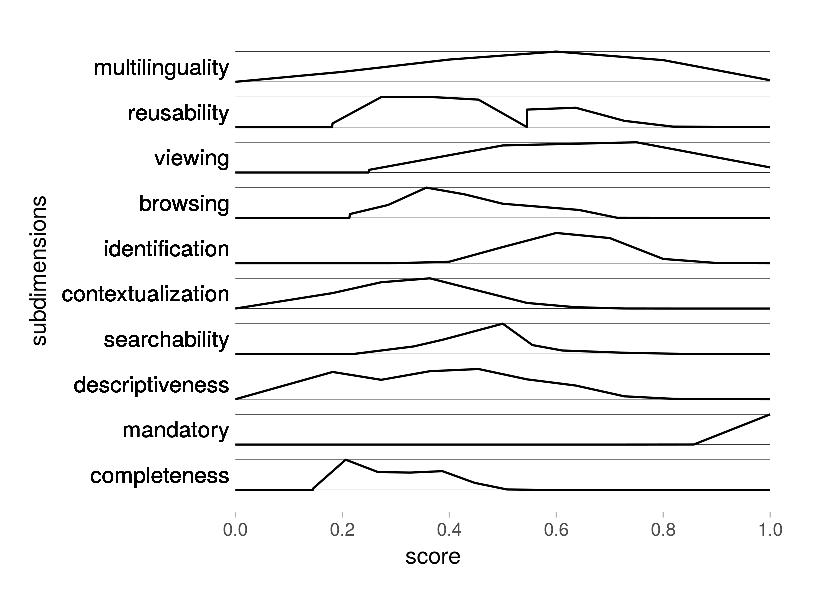
\includegraphics[width=\textwidth]{images/chapter02/subdimensions.eps}
\centering
\caption{The distribution of sub-dimension and 'simple completeness' scores}
\label{fig:subdimensions}
\end{figure}

In the second approach, the main factor is the normalized version of cardinality to prevent the biasing effect of extreme values. Sometimes there are more than one hundred or even a thousand field instances in a single record which would have too much effect on the score, so the tool normalizes them according to table \ref{table:normalization}.

\begin{table}
\caption{Normalization of cardinality}
\label{table:normalization}
\centering
\begin{tabular}{l|c|c|c|c|c}
number of instances & 0 & 1 & 2-4 & 5-10 & 11- \\
\hline
normalized score & 0.0 & 0.25 & 0.50 & 0.75 & 1.0 \\
\end{tabular}
\end{table}

The cardinality-based weight is simple: each field equally counts 1, but the rdf:about field (which identifies the individual entities) counts 10 so that the number of entities is taken into account for the weighting. The equation is

\begin{equation}
c_{cardinality} = \frac{\sum\limits_{i=1}^{d} norm(cardinality_i) \times weight_i}{\sum\limits_{i=1}^{d} weight_i}
\end{equation}

with $d$ as the number of fields, $cardinality_{i}$ as the cardinality of a field, $norm()$ as the normalizing function (see table \ref{table:normalization}) and $weight_i$ as the weight of a field in this computation.

The final equation is the combination of these two approaches where the first approach has a higher weight (so it is more important) than the second one:

\begin{equation}
c_{compound} = \frac{c_{sub-dimensions} + (0.4 \times c_{cardinality})}{1.4}
\end{equation}

\subsection{Implementation}

The data processing workflow has four phases. The current workflow ingests data from a MongoDB database, and stores the extracted records in line-oriented JSON files either in a Linux file system or in a Hadoop File System (using the available resources there is no significant difference in performance between the two, but in other scenarios the Hadoop File System could be a better choice). The record level analyses are written in Java, using the Spark API\footnote{Metadata quality assessment library: https://github.com/pkiraly/ metadata-qa-api, Europeana specific extension: https://github.com/ pkiraly/europeana-qa-api, Apache Spark interface: https://github.com/ pkiraly/europeana-qa-spark. The APIs (and the MARC assessment tool) are available as compiled Java libraries within Maven Central Repository: https://mvnrepository.com/artifact/de.gwdg.metadataqa, so one could use it in 3rd party Java or Scala projects.}. It provides automatic and configurable multithreading, so the tool can make use of the available resources of the environment effectively (either if it is a single machine with a multicore processor or a high performance computing cluster with several nodes). The output of these calculations are CSV files, which are also indexed by Apache Solr for occasional record based retrieval. The tool's quality dashboard makes use of the search and retrieval functionalities in displaying the results, and finding records with given quality metrics. 

The third phase is a statistical analysis of the record level metrics. For datasets and data providers the software is written in R\footnote{source code: https://github.com/pkiraly/europeana-qa-r} and in the Scala implementation of Spark\footnote{https://github.com/pkiraly/europeana-qa-spark/tree/master/scala}. It reads the CSV files generated in the previous phase, and produces CSV and JSON files for storing the results of the calculations and image files for graphs, visualizing central tendencies or other statistical features of the data. R however has a weak point: it works exclusively in memory, so the size of memory limits the size of the dataset it can process. In terms creating statistics for the whole Europeana dataset this is insufficient. For this reason, Scala on Spark is used for all top level aggregations. Scala’s statistical capabilities are not that rich, however, so it does not produce all the metrics that R does.

The last phase is an online statistical dashboard, a light-weighted, PHP and JavaScript based website which displays the output of the previous phases.\footnote{source code: \url{https://github.com/pkiraly/europeana-qa-web}} The technical details of the workflow is documented in \cite{kiraly2015b}. All phases are run in a single commodity hardware (Intel Core i7-4770 Quad-Core processor with 32 GB DDR3 RAM, with Ubuntu 16.04 operating system) which were also used at the same time for other research and development projects, so making the calculations resource-effective was an important software design constraint.

The data source for this calculation is a snapshot of Europeana data. The first snapshot was created at the end of 2015, which contains 46 million records, 1747 datasets and 3550 data providers\footnote{the name of data providers has not been not normalized so far, some organizations have several different names.} (extracted from Europeana's OAI-PMH service). During the project's lifetime additional snapshots have been created, the latest one is from August 2018 (62 million records, 1.27 TB in total, the data source is a replica of Europeana's MongoDB database).\footnote{In order to make the research repeatable, three full data snapshots are available for download at http://hdl.handle.net/21.11101/0000-0001-781F-7 and the first one is archived for long term preservation at the Humanities Data Center, Göttingen: https://hdl.handle.net/21.11101/EAEA0-826A-2D06-1569-0. The format of these snapshot is JSON, one record per line.} DQC aims to introduce a monthly update cycle, so the time span between the updates of the Europeana production database and the refreshing of the data quality dashboard should not be more than one month.

\section{Results}

\subsection{Completeness}

A comparison of the scores of sub-dimension-based (where the field importance counts) and the field-cardinality-based approaches (where the number of field instances counts) reveals that they give different results. While they correlate by the Pearson's correlation coefficient of 0.59, their shape and ranges are different. Because of the nature of the calculation the compound score is quite close to the first approach and the cardinality-based calculation has smaller effect on the final score. The sub-dimension-based scores are in the range of 0.22 and 0.92 while cardinality based scores are in the range of 0.05 and 0.48. The details of the distribution are shown in table \ref{table:completeness_metrics} and figure \ref{fig:completeness}.

\begin{figure}[ht]
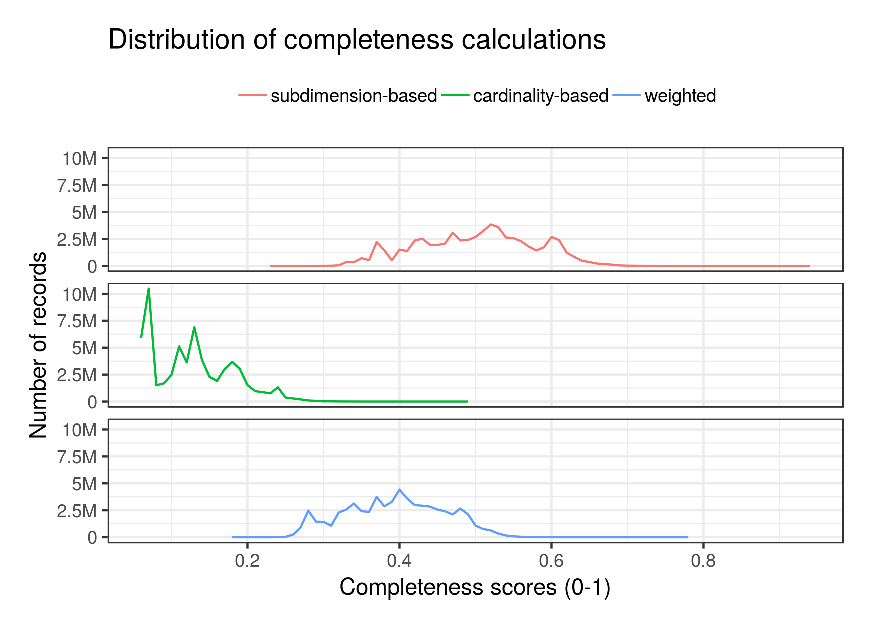
\includegraphics[width=\textwidth]{images/chapter02/completeness-score-histogram.eps}
\centering
\caption{Distribution of completeness calculations}
\label{fig:completeness}
\end{figure}

\begin{table}
\caption{Basic statistics of completeness calculations}
\label{table:completeness_metrics}
\centering
\begin{tabular}{l|c|c|c|c}
metric & mean & std.dev. & min. & max. \\
\hline
sub-dimension-based & 0.50 & 0.07 & 0.22 & 0.93 \\
cardinality-based & 0.12 & 0.05 & 0.05 & 0.48 \\
compound & 0.39 & 0.06 & 0.17 & 0.78 \\
\end{tabular}
\end{table}

There are data providers where all (in some cases more than ten thousand) records have the same scores: they have a uniform structure. Because one simple score is not enough to establish this, the field-level analysis shows that in these collections all the records have the very same (Dublin Core based) field set. On the other end there are collections where both scores diverge a lot. For example, in the identification of sub-dimension a data provider has five distinct values (from 0.4 to 0.8) almost evenly distributed while one of the best collections (of this category) is almost homogeneous: 99.7\% of the records have the same value: 0.9 (even the remaining 0.3\% has 0.8). This means that the corresponding fields\footnote{dc:title, dcterms:alternative, dc:description, dc:type, dc:identifier, dcterms:created, dc:date and dcterms:issued in the Provider Proxy and edm:provider and edm:dataProvider in the Aggregation.} are usually not available in the records of the first dataset, while they are almost always there in the second dataset. The tool provides different graphs and tables to visualize the distribution of the scores. 

From the distribution of the fields the first conclusion is that lots of records miss contextual entities, and only a couple of data providers have 100\% coverage (6\% of the records have \emph{agent}, 28\% have \emph{place}, 32\% have \emph{timespan} and 40\% have \emph{concept} entities). Only the mandatory technical elements appear in every record. There are fields, which are defined in the schema, but not filled in the records and there are overused fields – e.g. dc:description is frequently used instead of more specific fields (such as table of contents, subject related fields or alternative title).

Users can check all the features on the top, collection, and records level on the quality dashboard. Data providers get a clear view of their data, and based on this analysis they can design a data cleaning or data improvement plan.

\subsection{Multilinguality}

DQC has recently published details regarding the results of the multilinguality calculation (see \cite{charles2017} and \cite{kiraly-et-al2018}), so this section presents only a very short summary of the outcome. EDM follows the RDF model for language annotation, so data creators could denote that a string is written in a particular language (e.g. \emph{"Brandenburg Gate"@en}, where 'Brandenburg Gate' is the value of the field, and 'en' denotes English language). This construct is called a tagged literal. DQC found four relevant record-level metrics.

\begin{itemize}
 \setlength{\parskip}{0pt}
 \setlength{\itemsep}{0pt plus 1pt}
\item number of tagged literals
\item number of distinct language tags
\item number of tagged literals per language tags
\item average number of languages per property for which there is at least one language-tagged
\end{itemize}

These metrics were calculated for the Provider Proxy (which is the original data the organizations submit), the Europeana Proxy (which contains enhancements, typically from multilingual vocabularies), and finally for the whole object. The output is summarized in tables \ref{table:multilinguality_metrics} and \ref{table:multilinguality_distribution} and figure \ref{fig:multilinguality}).

\begin{table}
\caption{Metrics of multilinguality (means)}
\label{table:multilinguality_metrics}
\centering
\begin{tabular}{l|c|c|c}
metric & provider & europeana & whole object \\
\hline
number of tagged literals & 5.44 & 64.34 & 69.79 \\
\hline
number of distinct language & 1.67 & 37.92 & 38.79 \\
tags & & & \\
\hline
number of tagged literals & 2.64 & 0.95 & 2.17 \\
per language tags & & & \\
\hline
average number of languages & 1.10 & 28.10 & 20.21 \\
per property for which there & & & \\
is at least one language-tagged & & & \\
 literal & & & \\
\end{tabular}
\end{table}

\begin{figure}[ht]
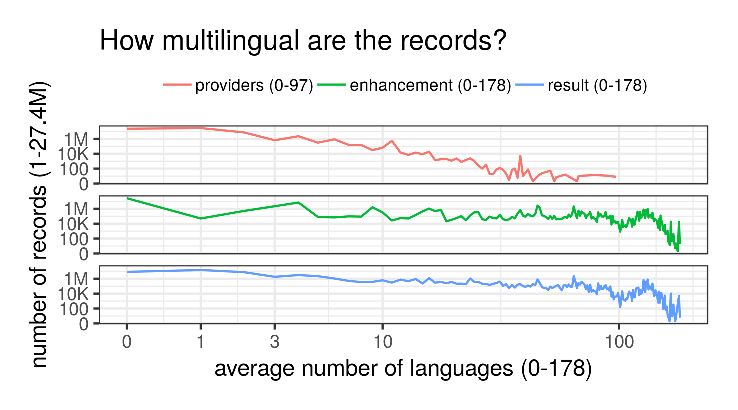
\includegraphics[width=\textwidth]{images/chapter02/multilinguality-summary.eps}
\centering
\caption{Multilinguality}
\label{fig:multilinguality}
\end{figure}

\begin{table}
\caption{Distribution of average number of languages per property}
\label{table:multilinguality_distribution}
\centering
\begin{tabular}{l|r|r|r}
entity & 0 & 1 & 2 or more \\
\hline
Provider Proxy & 22.4M (36.2\%) & 27.3M (44.1\%) & 12.1M (19.6\%) \\
Europeana Proxy & 25.8M (41.7\%) & 49K (0.07\%) & 36.1M (58.2\%) \\
Object & 8.2M (13.3\%) & 14.6M (23.7\%) & 39.1M (63.0\%) \\   
\end{tabular}
\end{table}

Table \ref{table:multilinguality_distribution} reflects that only 20\% of the records have two or more languages per property in the Provider Proxy. After the enhancement process injects external contextual information (about agents, concepts, places and timespans) from multilingual data sources such as DBpedia and other sources into the Europeana records, the overall multilinguality became higher. Not only are the number of fields with two or more language values increased, but the number of records without any language annotation also decreased.

Another finding is that the language tags are not always standardized. Different data providers follow different standards, or use ad-hoc tags. In the whole dataset there are more than 400 different language tags, but several tags denote the same language (e.g. "en", "eng", "Eng" etc. refer to English). A further investigation should analyze records with normalized language tags, to get a more thorough picture of language usage.

\subsection{Uniqueness}

One might recall the example of similar titles mentioned at the beginning of this paper. To find those records we should calculate the uniqueness of the values. Uniqueness is a positive value in those fields which should describe unique properties of an object, and less positive (or even negative) in those fields which connects records to contextual information where the values should come from a controlled vocabulary, and thus in an ideal case multiple records will share the same terms. In order to effectively establish the uniqueness of a value, one should be able to check a search index with the special requirement that it should index and store field values as a phrase. Since building such an index for the whole dataset would have required more resources than were available for this research, three fields were selected for this task: title, alternative title, and description. In calculating this score we applied a modified version of Solr's relevancy scoring:

\begin{equation}
score(t_f, v_f) = log\left(1 + \frac{t_f - v_f + 0.5}{v_f + 0.5}\right)
\end{equation}

\begin{equation}
uniqueness_f = \left(\frac{score(t_f, v_f)}{score(t_f, 1.0}\right)^3
\end{equation}

$t_f$ is the number of records where field $f$ is available, $v_f$ is the frequency of a value.

As seen in figure \ref{fig:uniqueness-theoretical} the score decreases radically as the field value became more frequent. On the user interface there is a categorization: besides the unique values, there are 5 categories denoted with stars. Table \ref{table:uniqueness-boundaries} displays the category boundaries for these three fields:

\begin{table}
\caption{Uniqueness categories by frequency}
\label{table:uniqueness-boundaries}
\centering
\begin{tabular}{l|c|c|c|c|c}
field & ***** & **** & *** & ** & * \\
\hline
title & 2- & 8- & 37- & 293- & 5226- \\
alternative & 2- & 6- & 23- & 132- & 1514- \\
description & 2- & 7- & 34- & 252- & 4128-
\end{tabular}
\end{table}

\begin{figure}[ht]
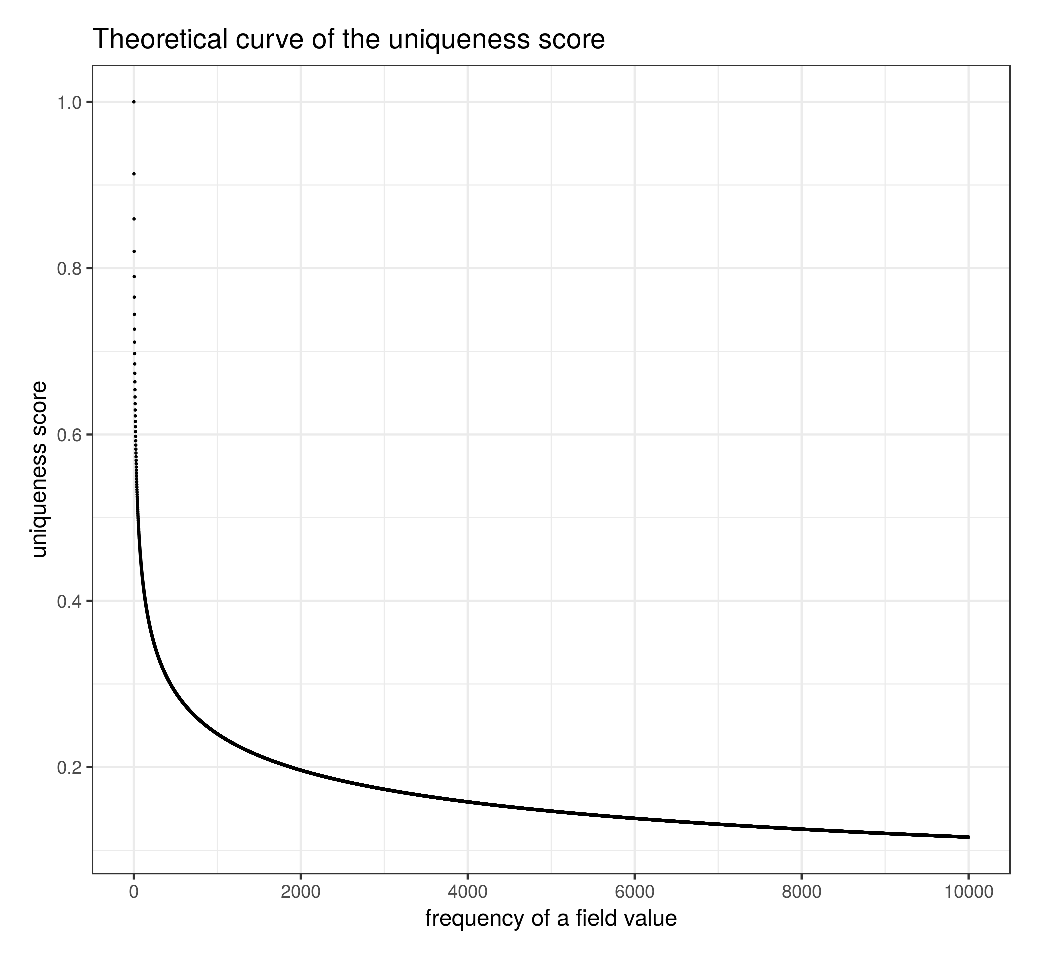
\includegraphics[width=\textwidth]{images/chapter02/uniqueness-theoretical.eps}
\centering
\caption{Theoretical curve of uniqueness score. As frequency of terms gets higher, the uniqueness score get radically smaller towards zero.}
\label{fig:uniqueness-theoretical}
\end{figure}

The result of the categorization is shown in table \ref{table:uniqueness-result}. While the absolute majority of the records in regards to all three fields do contain unique values, there are still millions of records with low scores for one or another field, and moreover there are almost ten thousand records where none of these fields are available. When we examine the three values together (see the last row of the table), and calculate an average of the result, we find that there are 25 million records with unique values in all available fields while on the other side of the scale only 3.62\% of the records are in the lowest category. This means that even if some values are low, most of the time there is at least one field with a less frequent value, so the record has a higher chance to be found by a search term.

\begin{table}
\caption{How unique are Europeana records?}
\label{table:uniqueness-result}
\centering
\begin{tabular}{l|c|c|c|c|c|c}
field & unique & ***** & **** & *** & ** & * \\
\hline
title & 59.4 & 9.5 & 8.3 & 8.7 & 7.1 & 6.6 \\
alternative & 62.4 & 11.2 & 7.1 & 3.6 & 2.7 & 12.7 \\
description & 54.6 & 9.0 & 7.3 & 10.2 & 6.7 & 11.9 \\
together & 45.4 & 10.8 & 15.6 & 18.2 & 6.3 & 3.62
\end{tabular}
\end{table}

From the Solr index we could extract the most frequent terms. Along with the "photograph" example in the introduction there are many frequent phrases in the title field denoting missing information (e.g. "Unbekannt", "Onbekend" or "+++EMPTY+++"), collection, journal or institution names ("Journal des débats politiques et littéraires", "ROMAN COIN") or even a general descriptive term ("Porträtt", "Château", "Plakat", "Rijksmonument"). It would require further investigation to filter out those frequent terms which appear in records especially where the other descriptive fields also lack a necessary level of uniqueness. The tool described here provides a solid basis for such an investigation.

\subsection{Record patterns}

What fields make up a typical record? In other words: what fields do data providers actually use? Record patterns are the typical field collocations. Since the completeness measurement counts the existence of all the fields, a map-reduce based analysis could extract these patterns. In this case the mapping function creates the patterns (each pattern is a list of field names available in a particular record) while the reduce-function counts them. In the first iteration it turned out that there were too many similar patterns worthy of grouping together in order to analyze them effectively. A similarity algorithm was therefore applied for clustering the patterns. All patterns were first represented by a string containing zeros and ones. First, all the fields of a collection were collected and sorted by a standard field order. Each field was then categorized into one of three categories: mandatory fields, important fields (those fields which appeared in a sub-dimension) and non-important fields. If the field exists in the pattern it is represented by one or more ones otherwise one or more zeros. The mandatory fields get three characters, the important fields get two, and others gets only one character. This way the patterns having the same important fields and different unimportant fields are closer to each other than patterns sharing the non-important fields. The similarity is calculated by the Jaro-Winkler algorithm. In the visualization (as you can see in figure \ref{fig:patterns}) the clusters are displayed by default, and the user needs to click to display the patterns belonging to a cluster. The table is ordered by the number of records, so the more typical records are on the top. If the field is only available in some records within the cluster, it is grayed (the color is proportional with the number of records). By default the page does not display patterns occuring in less than 1\% of the records.

\begin{figure}[ht]
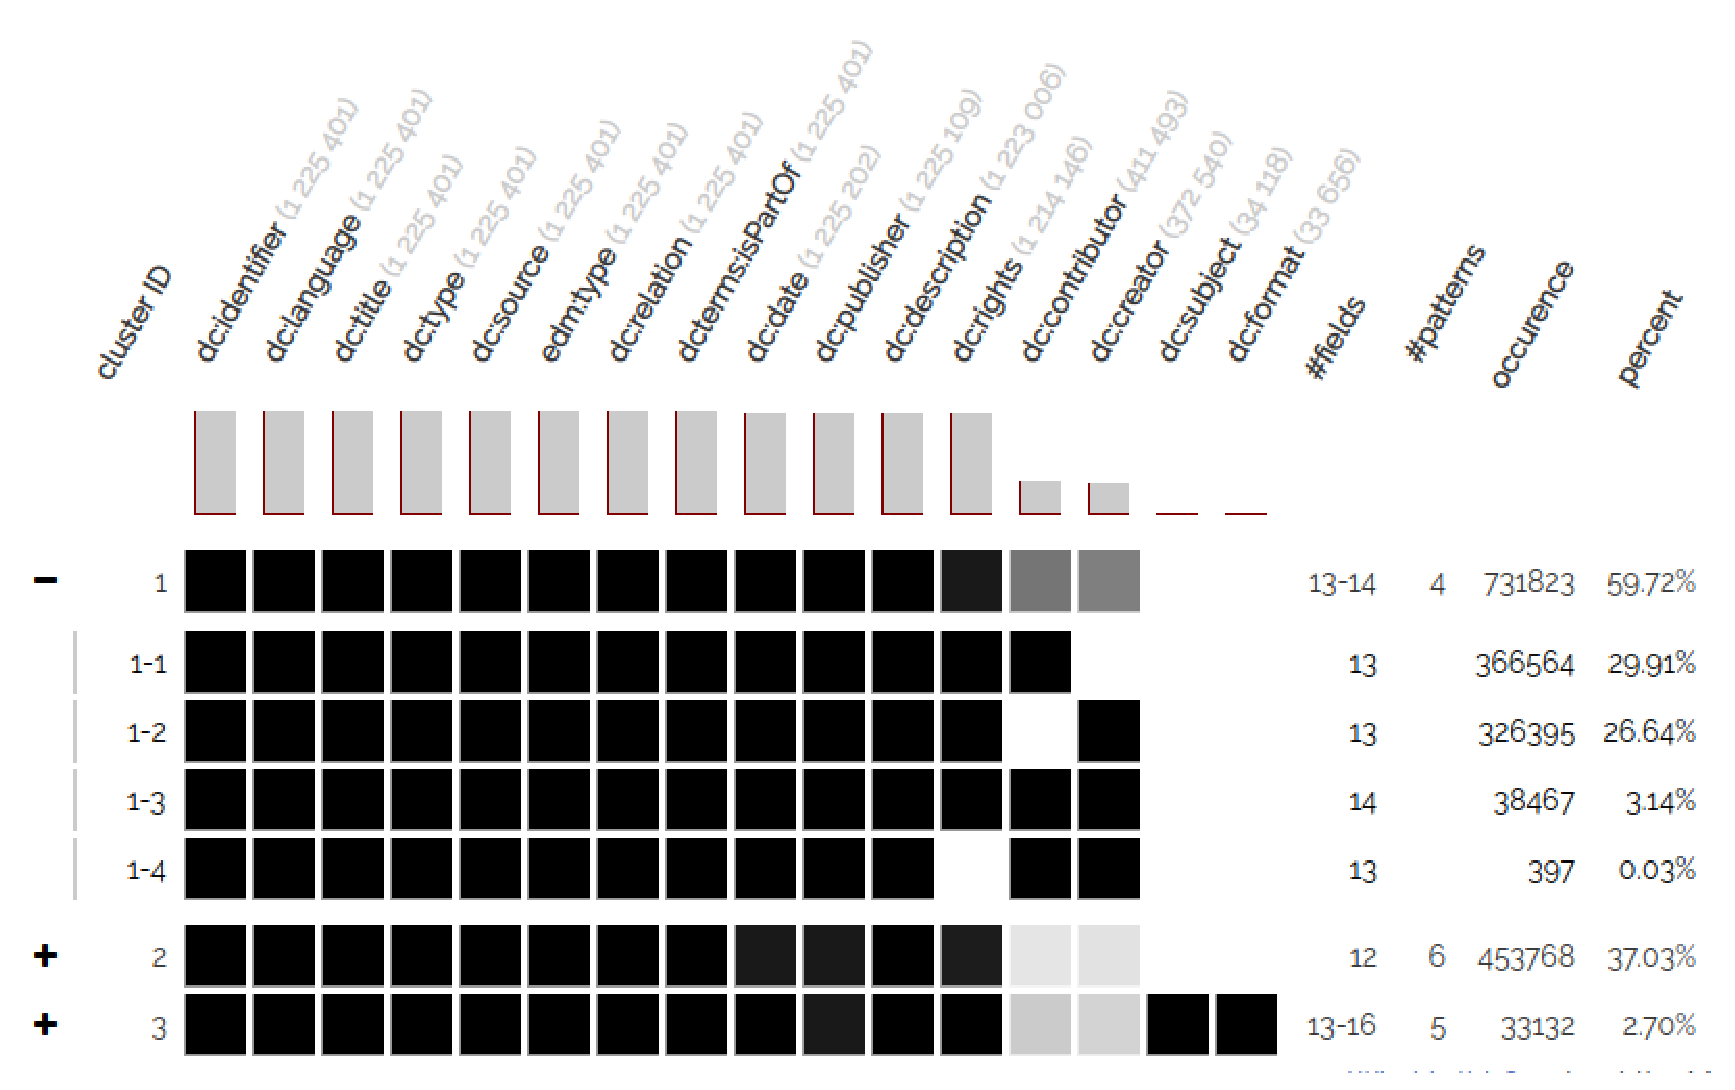
\includegraphics[width=\textwidth]{images/chapter02/clustered-patternsv05.eps}
\centering
\caption{Clustered record patterns. The first line represents a cluster of similar patterns. The next four lines are the patterns belonging to the cluster. The top gray bar represents the frequency of fields in the whole collection.}
\label{fig:patterns}
\end{figure}

Thus far two quality problems were revealed by the use of record patterns. The first problem covers those records which had only a small number of fields. There were more than $150,000$ records having only the following four fields in the Provider Proxy entity: dc:title, dc:type, dc:rights, and edm:type, of which only the first two might contain descriptive information about the object. It is evident that there is a high chance that users would not be able to discover these records by using facets, due to the lack of descriptive information about the object. The second problem is structural homogeneity: each record in some collection always has the same set of fields. There are 906 such data providers in Europeana, but fortunately most of them are relatively small collections, only 26 have more than a thousand records. The biggest homogeneous collection (with over $500,000$ records), however, contains only 5 fields (of which 3 are descriptive). The problem with such a record is that it contains generic fields instead of specific ones (for example it does not make distinctions among conceptual, spatial and temporal subject headings, and puts different contextual information into dc:type or dc:subject).

\section{Further work}

Europeana is currently working on its new ingestion system called Metis\footnote{https://github.com/europeana/metis-framework}, and it will able to integrate the tool described here. It is currently planned that when a new record-set arrives for import the measurement will be launched automatically. The Ingestion Officer can then check the quality report and share both the output and general conclusions with data providers who can then either change their transformation rules or hopefully fix issues with their metadata records if possible.

There are other metrics in addition to the calculation models that were discussed in this paper, and we are planning to compute them in the near future (e.g. accuracy, information content, timeliness, existence of known metadata anti-patterns). Much of the related literature suggests calculating a top level score, which summarizes all metrics into one final score that characterizes the record’s metadata quality. This could be achieved by weighting the metrics or applying machine learning algorithms, such as Principal Component Analysis \cite{james2013}. It was mentioned previously that the current completeness calculation approach only confirms the existence of a field. The next step on this research front is to extend this model with content evaluation of the relevant fields according to the User Scenarios analysis (\cite{hill-charles-isaac2015}).

In DQC, we also plan to compare the scores with experts’ evaluation and with usage data (log files). Harper ran a test to reveal whether there is a correlation between the usage of an object (the frequency of access via their portal and API) and the scores calculated by a quality assessment conducted by the Digital Public Library of America (which is similar to Europeana regarding to its purpose and its metadata schema). This approach failed partly because there was not enough usage data available at time the research was conducted, however, the proposed method sounds promising, and if Europeana has log files it would be worthwhile to run an experiment.

Other future plans include defining the problem catalogue with W3C’s Shapes Constraint Language \cite{knublauch2017} and publishing the results as linked data fitted to the Data Quality Vocabulary Ontology \cite{albertoni-isaac2016}.

The proposed method could also be used in data collections using other metadata schemas, such as MARC based library catalogues\footnote{Since MARC has lots of strict content related rules, and EDM only has a few, there is a significant distance between the approaches followed in the two projects.}, EAD-based archival collections,\footnote{The biggest European archival collection Archives Portal Europe (http://www.archivesportaleurope.net/) published their data via a REST API under CC0 license.} and others.

\section{Conclusion}

This research sought to rethink the relationship between functionality and metadata schema (together with the DQC) and a framework was implemented that proved successful in measuring structural features that correlate with metadata issues. The user of the framework is able to select between low and high quality records. According to our original hypothesis, structural features such as field existence and cardinality correlated with metadata quality, and this ultimately proved to be true. In addition, this work also extended the volume of records analyzed by introducing big data tools that were not mentioned previously in the literature.

Although this research focused on a particular dataset and metadata schema, the applied method is based on generalized algorithms so it could also be applied to other data schemas. Several Digital Humanities studies (some examples: KOLIMO (Corpus of Literary Modernism)\footnote{https://kolimo.uni-goettingen.de/}, \cite{strezoski2017}, \cite{schmidt2017}) based on schema defined cultural databases. The research process could also be improved by finding the weak points of the sources, making the conclusions more reliable, and -- reflecting on Felix Rau's tweet quoted at the beginning of this paper -- by forming more realistic assumptions about the data.

\section*{Acknowledgment}
The first author would like to thank to all the past and current members of the Europeana Data Quality Committee, to the supervisors of his PhD research, Gerhard Lauer, and Ramin Yahyapour, to Jakob Voß, Juliane Stiller, Mark Phillips for providing feedback, to Christina Harlow and Zaveri Amrapali for general inspiration, and to Felix Rau for the motto and to GWDG for supporting the research.

% \bibliographystyle{acm}
% \bibliography{bibliography-for-papers}

\chapter[Evaluating Data Quality in Europeana: Metrics for Multilinguality]{Evaluating Data Quality in Europeana: Metrics for Multilinguality\footnote{This chapter has been published as \cite{kiraly-et-al2018}.}}
\chapterauthor{Péter Király, Juliane Stiller, Charles Valentine, Werner Bailer, and Nuno Freire}


\emph{Abstract}: Europeana.eu aggregates metadata describing more than 50 million cultural heritage objects from libraries, museums, archives and audiovisual archives across Europe. The need for quality of metadata is particularly motivated by its impact on user experience, information retrieval and data re-use in other contexts. One of the key goals of Europeana is to enable users to retrieve cultural heritage resources irrespective of their origin and the material's metadata language. The presence of multilingual metadata description is therefore essential to successful cross-language retrieval. Quantitatively determining Europeana's cross-lingual reach is a prerequisite for enhancing the quality of metadata in various languages.
% * <nfreire@gmail.com> 2018-06-11T17:47:34.061Z:
% 
% > quality
% availability
% 
% ^ <nfreire@gmail.com> 2018-06-11T17:47:54.531Z.
Capturing multilingual aspects of the data requires us to take into account the full lifecycle of data aggregation including data enhancement processes such as automatic data enrichment.The paper presents an approach for assessing multilinguality as part of data quality dimensions, namely completeness, consistency, conformity and accessibility. We describe the measures defined and implemented, and provide initial results and recommendations. 

%\keywords{metadata quality, multilinguality, digital cultural heritage, Europeana, data quality dimensions}

%\end{abstract}
%
\section{Introduction}
Europeana.eu\footnote{\url{http://www.europeana.eu/}} is Europe's digital platform for cultural heritage. It aggregates metadata describing more than 50 million cultural heritage objects from a wide variety of institutions (libraries, museums, archives and audiovisual archives) across Europe. 
The need for high-quality metadata is particularly motivated by its impact on search, the overall Europeana user experience, and on data re-use in other contexts such as the creative industries, education and research. One of the key goals of Europeana is to enable users to find the cultural heritage objects that are relevant to their information needs irrespective of their national or institutional origin and the material's metadata language. 

As highlighted in the White Paper on Best Practices for Multilingual Access to Digital Libraries~\cite{stiller2016}, most digital cultural heritage objects do not have a specific language, i.e., as they are not in textual form, and can only be searched through their metadata, which is text in a particular language. The presence of multilingual metadata description is therefore essential to improving the retrieval of these objects across language spaces. Quantitatively determining Europeana's cross-lingual reach is a prerequisite for enhancing the quality of metadata in various languages.

%In the Data Quality Committee (DQC), a body formed at Europeana's initiative, we specify functional requirements that define the purpose of the metadata and guide data-quality evaluation -- following a core principle for metadata assessment (e.g.~\cite{guy2004}). Europeana's international scope means that multilinguality is an inherent aspect of these requirements.  

In this paper, we present multilinguality as a 
measurable component of different data quality dimensions: completeness, consistency, conformity and accessibility. We capture data quality by defining and implementing quality measures along the full data-aggregation lifecycle, taking also into account the impact of data enhancement processes such as semantic enrichment. The model the data is represented in, namely the Europeana Data Model (EDM)\footnote{\url{http://pro.europeana.eu/edm-documentation}}, is also a key element of our work. 

In the next section, we present data quality frameworks, dimensions and criteria that are commonly referred to in the context of data quality measurement. Section 3 describes how multilingual metadata is presented in Europeana's data model and the data quality dimensions we use are also introduced. In Section 4, we describe the implementation of the different measures as well as the calculation of the scores. Section 5 describes first results and measures that were taken to improve metadata along the different quality dimensions and the first recommendations we have been able to identify based on the results from the metrics. We conclude this paper with an outline of future work. 

\section{State of the art}

Addressing data quality requires the identification of the data features that need to be improved and this is closely linked to the purpose the metadata is serving. Libraries have always highlighted that bibliographic metadata enables users to find material, to identify an item and to select and obtain an entity~\cite{frbr1998}. Based on this, Park~\cite{park2009} expands functional requirements of bibliographic data to discovery, use, provenance, currency, authentication and administration, and related quality dimensions. The approach to metadata assessment for cultural heritage repositories presented in~\cite{bellini2013} also starts from use for a specific purpose. While the work mentions the issue of multilinguality, it does not propose specific metrics to measure it.

Different sets of dimensions have been proposed for classifying metadata quality measures. Bruce and Hillmann~\cite{bruce-hillmann2004} define the following measures for quality: completeness, accuracy, provenance, conformance, logical consistency and coherence, timeliness and accessibility,
%, grouped in three tiers. However, 
multilinguality is not addressed in this work. %Shreeves et al.~\cite{shreeves2005} focus on three quality dimensions (completeness, consistency and ambiguity) for their explorative study of four collections, which included metadata from several institutions. 
%Not surprisingly, they found greater variances for collections aggregated from multiple sources as well as inconsistencies in the encoding scheme -- a result also experienced by Europeana. They also report very low use of language elements in the collections they analysed. 
%Designing an information quality framework, Stvilia et al.~\cite{stvilia_2007} have proposed a taxonomy of 22 measures, grouped into three categories: intrinsic, relational/contextual and reputational information quality. 
%In this taxonomy, completeness/precision exists both in the intrinsic (e.g.\ the number of elements, the non-empty elements) and in the relational/contextual categories (completeness wrt.\ a recommended set of elements). Although multilinguality is not explicitly mentioned in this paper, it fits in this model as part of contextual completeness.
The existing works that consider multilinguality assign it to different quality dimensions, depending on the purpose of the measurement. Zaveri et al.~\cite{zaveri2015} propose dimensions for quality assessment for linked data.
%, grouped into the accessibility, intrinsic, contextual and representational categories.
Completeness is listed as an intrinsic criterion, while multilinguality is covered by versatility, which is considered a representational criterion. The ISO/IEC 25012 standard~\cite{iso25012} defines a data quality model with 15 characteristics, discriminating between inherent and system-dependent ones, but putting many of the criteria in the overlap between the two classes. Completeness is defined as an inherent criterion, while accessibility and compliance (conformity) are in the overlapping area. Multilinguality could be seen as being compliant to providing a certain number of elements in a certain number of languages, and as enabling access to users who are able to search and understand results in certain languages.
Radulovi\'c et al.~\cite{radulovic2017} propose a metadata quality model for linked data, and define multiple languages as an indicator for the quality dimension availability, i.e., can it be accessed by users with the requirement to get the data in a specific language. Ellefi et al.~\cite{ellefi2017} propose a taxonomy of features for profiling RDF datasets, of which one part discusses quality. %Similar to Zaveri et al.~\cite{zaveri_2015}, t
They define representativity as one dimension of quality in their model, under which they see versatility (including multilinguality) as one measure.
%A slightly different but related topic is measuring multilinguality of vocabularies or thesauri. Mader et al.~\cite{mader2012} include issues related to multilinguality, such as incompleteness of language coverage and missing language tags, in their analysis of SKOS vocabularies. Multilinguality is covered by Dr\"oge \cite{droge2012} as part of the eight classes of criteria defined for assessing the quality of vocabularies. However, no metric is developed in detail.
% this paragraph was commented in the TPDL paper, as it is not on the core topic of the paper
%Apart from measuring quality, the representation of quality analysis results in an interoperable way is an important question. \cite{debattista2016} propose an extensible framework for assessing quality of Linked Open Data called Luzzu. One important contribution of their work is a data quality ontology (daQ), which was also used an input to W3C’s recent work on a vocabulary to describe data quality \cite{albertoni_isaac_2016}.
To the best of the authors' knowledge, the only resource which actually measured multilingual features in metadata is~\cite{vogias2013}, cited in \cite{palavitsinis2014}. %Here language attributions across a collection were counted. However, this work only considers multilinguality of free text fields, but not the use of multilingual controlled vocabularies. 
Albertoni et al.~\cite{albertoni2015} also include multilinguality in a scoring function, although in the context of importing other linked data vocabularies. %They propose a scoring scheme in which additional alternative labels and labels in other languages increase the quality score given to a SKOS vocabulary. In the context of measuring the quality of Wikipedia articles, multilinguality has also been considered as input to scoring~\cite{hammwohner2007}. However, this work rather focuses on the existence of links between different language versions and the consistency between them. 

It becomes apparent that while multilinguality is considered in some works, it is usually not treated as a separate quality dimension, but rather as part of other criteria or dimensions existing at quite different levels in different quality models. %Palavitsinis~\cite{palavitsinis_2014} provides a detailed overview of the dimensions used in the literature of more than a decade (this list also containing obviously strongly overlapping dimensions such as ``accuracy'' and ``correctness''). This work also compares definitions of (meta)data quality, of which many agree that quality is driven by satisfying specific need, while other focus on a accurate and complete representation. This indicates the same discrepancy as the assignment of multilinguality to a specific quality dimension, either as an enabler of an application or for ensuring the completeness and accuracy of the description.
We use the measures based on the frequency of language tags described in~\cite{vogias2013} as a basis, and following the conclusion from the literature, consider multilinguality in the context of different quality dimensions. Our work started with the development of metrics to measure the multilingual quality of metadata in Europeana within the EU-funded project Europeana DSI-2\footnote{\url{https://pro.europeana.eu/project/europeana-dsi-2}}. 
%Following a theoretical framework described in the project deliverable~\cite{stiller2017}, 
A first iteration of a multilingual saturation score that counted language tags across metadata fields in the Europeana collections as well as the existence of links to multilingual vocabularies was introduced by Stiller and Király~\cite{stiller-kiraly2017}. The score was extended in~\cite{charles2017} by including measures that define multilinguality as part of different quality dimensions. 
%The further development of these metrics as well as the integration of measures for all aspects of multilingual data is described in this paper. The implementation and operationalisation of the measures into the metadata quality assurance framework \cite{kiraly_2017} will be presented as well as results.
\section{Approach}
Firstly, to determine the multilingual degree of metadata across several quality dimensions, we have to understand the different ways multilingual information is expressed in Europeana's data model. Secondly, the structure of multilingual data informs the criteria and metrics that enable us to measure multilinguality across several metadata quality dimensions.
\subsection{Multilingual information in Europeana's metadata}
\label{sec:multilingualinfo}

Multilinguality in Europeana's metadata has two perspectives: concerning the language of the object itself, and the language of the metadata that describes this object. First, the described cultural object, insofar as it is textual, audiovisual or in any other way a linguistic artefact, has a language. The data providers are urged to indicate the language of the object in the \textit{dc:language} field in the Europeana Data Model (EDM) in this way: \texttt{<dc:language>de</dc:language>}. If used consistently and in accordance with standards for language codes, this information could then be used to populate a language facet allowing users to filter result-sets by language of objects. The language information is essential for users who want to use objects in their preferred language. 
Second, the language of metadata is essential for retrieving items and determining their relevance. Metadata descriptions are textual and therefore have a language. Each value in the metadata fields can be provided with a language tag (or language attribute). Ideally, the language is known and indicated by this tag for every literal in each field. If several language tags in different languages exist, the multilingual value can be considered to be higher. For instance, consider as an example this data provided by an institution:

\begingroup
   \fontsize{8pt}{10pt}\selectfont
\begin{verbatim}
<#example> a ore:Proxy ;  # data from provider
  dc:subject "Ballet",    # literal
  dc:subject "Opera"@en . # literal with language tag
\end{verbatim}
\endgroup

The first \textit{dc:subject} statement is without language information, whereas the second tells us that the literal is in English. Multilingual information is not only provided by the institutions but can also be introduced by Europeana.
Europeana assesses metadata in particular fields to enrich it automatically with controlled and multilingual vocabularies as defined in the Europeana Semantic Enrichment Framework.\footnote{\url{https://docs.google.com/document/d/1JvjrWMTpMIH7WnuieNqcT0zpJAXUPo6x4uMBj1pEx0Y/edit}} As shown in the following example, the dereferencing of the link (i.e., retrieving all the multilingual data attached to concepts defined in a linked data service) allows Europeana to add the language variants for this particular keyword to its search index.

\begingroup
   \fontsize{8pt}{10pt}\selectfont
\begin{verbatim}
<#example> a ore:Proxy ; edm:europeanaProxy true ;
  # enrichment by Europeana with multilingual vocabulary
  dc:subject <http://data.europeana.eu/concept/base/264> . 
 
<http://data.europeana.eu/concept/base/264> a skos:Concept ;
  # language variants are added to index
  skos:prefLabel "Ballett"@no, "Ballett"@de, "Balé"@pt, 
                 "Baletas"@lt, "Balet"@hr, "Balets"@lv .
\end{verbatim}
\endgroup
The record now has more multilingual information than at the time of ingestion into Europeana. The labels are added to the search index and this particular record can be retrieved with various language variants of the term \textit{ballet}. The different language versions from multilingual vocabularies are likely to be translation variants. This distinction between the provided metadata and the metadata created by Europeana needs to be taken into account for measuring multilinguality as defined in Section~4. 

%\subsection{Functional requirements for multilingual services}
%The definition of multilingual services requires to better understand the impact of multilinguality on the search and discovery of resources as well as on the overall user experience. We have therefore identified multilingual aspects in several functional requirements relevant to Europeana. Note that these requirements are also crucial to better communicating the results of our measures to Europeana's data providers, and hence to motivating improvement of the data.

%\noindent\textbf{Cross-language recall:} when a user wants to search for a document or documents relevant to her needs, and to do so irrespective of the language of the documents and/or their metadata, multilingual metadata is a necessity. This requirement is fundamental for Europeana as users should be able to find what they are looking for, based on their informational needs. This use case can be supported by two different search scenarios: 
%\begin{enumerate}
%\item Topical (or informational) search - in this context, the user's query is motivated by a problem. 
%\item Known-item search - the user's query is concrete looking for a particular item. 
%\end{enumerate}

%\noindent For those two scenarios, answers to user queries will be supported by metadata elements providing topical and contextual information. Therefore we consider that the metadata quality for all metadata description must be as high as possible in terms of:
%\begin{itemize}
% \setlength{\parskip}{0pt}
% \setlength{\itemsep}{0pt plus 1pt}
%\item [$-$] Completeness: all relevant metadata elements should be supplied with values. 
%\item [$-$] Consistency: Metadata values must be correct and appropriate to their metadata elements and consistently used across a dataset or a collection.
%\item [$-$] Conformity: Metadata should be ideally taken from a controlled vocabulary or encoded according to a given standard. 
%\item [$-$] Accessibility: all relevant metadata elements should be supplied in the user's preferred language.
%\end{itemize}
%However, in order to fulfil our requirement all these dimensions should be applied to multilinguality. Our scenario requires not only that that all searchable free-text metadata elements are present\footnote{ \url{https://docs.google.com/spreadsheets/d/1f6vbeo4mt0stl0yAbVCyp_-5bzBBCq4Dy6p7xhMcjSI/}}, consistent and in accordance with standards but also that they are tagged with their language.\footnote{ For instance, in accordance with the ISO 639-1 or 632-2 (\url{https://www.loc.gov/standards/iso639-2/php/code_list.php}) list, the IANA language tag registry (\url{http://www.iana.org/assignments/language-subtag-registry/language-subtag-registry}), or the Languages Name Authority List (NAL) (\url{https://open-data.europa.eu/en/data/dataset/language})}

%\noindent\textbf{Language based facets:} these facets allow users to filter results sets either by the language of the object or by the language of the describing metadata. In this requirement, a clear distinction needs to be made between the language that refers to the language of the metadata and the language of the digital representation of the work. While the language of the metadata will be measured against the presence of language tags, the language of the content will be captured in the \textit{dc:language} field in EDM. The existence of multilingual metadata records in Europeana demands that language-tagging occurs at the level of the metadata element rather than the record as a whole. Europeana needs language tags to be applied consistently to avoid the dominance of some languages over others. In the Europeana context, the completeness of language based facets would require the presence of all the official languages of the European Union \footnote{ \url{https://europa.eu/european-union/about-eu/figures/administration_en\#goto_2}}. 
%The presence of additional languages would facilitate the accessibility of the Europeana collection. 

%\noindent\textbf{Entity-based facets:} these facets allow users to refine their results by people, places, concepts and periods associated with Cultural Heritage Objects (CHO). The search performed in this context returns more accurate results and therefore decreases the number of results a user is confronted with in Europeana. This requirement involves the presence of relationships between a CHO and one or more entities represented as a fully-fledged resource (Agents, Places, Concepts, etc.). 
%While users will be primarily searching for entities in their own language (e.g. the city of \textit{Paris}), they will need to access results in different languages (\textit{Parijs, Parigi, ...}). To support this scenario, we will rely on the translated labels provided by data providers as part of their metadata or on multilingual vocabularies to which monolingual metadata can be linked. In both cases, it is crucial to quantify multilinguality to identify language gaps.

\subsection{Multilinguality as a facet of quality dimensions}
For measuring multilinguality, we identify four quality dimensions: completeness, consistency, conformity and accessibility. Each of these dimensions assesses multilinguality from a different perspective. 

\noindent\textbf{Completeness.}
Completeness is a basic quality measure, expressing the number (proportion) of fields present in a dataset, and identifying non-empty values in a record or (sub-)collection. For a fixed set of fields completeness is thus straightforward to measure, and can be expressed as the absolute number or fraction of the fields present and not empty. However, the measure becomes non-trivial when data is represented using a data model with optional fields (that may e.g., only be applicable for certain types of objects), or with certain fields for which the cardinality is unlimited (e.g., allowing zero to many subjects or keywords). These characteristics apply to EDM. In such cases the measure becomes unbounded, and a few fields with high cardinality may outweigh or swamp other fields. 

In the context of measuring multilingual completeness, the metric is two-fold. First, the concept of completeness can be applied to measuring the presence of fields with language tags. This measure of multilinguality must be seen in relation to the results of measuring completeness. Only fields both present and non-empty can be said to have or lack language tags and translations. A record which is 80\% complete can still reach 100\% multilingual completeness if all present and non-empty fields have a language tag.
Second, the completeness measure can reflect the presence of the \textit{dc:language} field that identifies the language of the described object.

\noindent \textbf{Consistency.}
Consistency describes the logical coherence of the metadata across fields and within a collection. With regard to multilinguality, the dimension assesses the variety of language values in the \textit{dc:language} field and the language tags that specify the language in a given field. Consistent values should be used to describe the same language.

In Europeana, the consistency measure for the \textit{dc:language} field is mainly relevant for the language based facet. The more consistent languages are expressed, the more useful language facets become. Ideally, inconsistencies in expressing languages through language codes should be fixed through normalization (see Section~\ref{sec:results}).

\noindent \textbf{Conformity.}
Conformity refers to the accordance of values to a given standard or a set of rules. Here, the language values in the \textit{dc:language} field and the language tags in any given field can be assessed with regard to their conformity to a given standard such as ISO-639-2\footnote{ \url{https://www.loc.gov/standards/iso639-2/php/code_list.php}}.
The conformity measure for the \textit{dc:language} field influences the usefulness of a language facet. 

\noindent\textbf{Accessibility.}
Accessibility describes the degree to which multilingual information is present in the data, and allows us to understand how easy or hard it is for users with different language backgrounds to access information. So far, Europeana has little knowledge about the distribution of linguistic information in its metadata -- especially within single records. To quantify the multilingual degree of data and measure cross-lingual accessibility, the language tag is crucial. The more language tags representing different languages are present, the higher is the multilingual reach. Resulting metrics can be scaled to the field, record and collection levels. In practical terms, the accessibility measure serves to gauge cross-language recall and entity-based facet performance.
To summarize: with regard to multilinguality, we identified the dimensions, quality criteria and measures presented in Table~\ref{Tab:dimensions}.

\begin{table}[tb]
\caption{Dimensions, criteria and measures for assessing multilinguality in metadata.}
\centering
\begin{tabular}{ l p{4.5cm} p{5.5cm} }
\hline\noalign{\smallskip}
\multicolumn{1}{l}{\bfseries Dimension} &
\multicolumn{1}{l}{\bfseries Criteria} &
\multicolumn{1}{l}{\bfseries Measures} \\
%\noalign{\smallskip}
% \hline
\hline
%\noalign{\bigskip}
Completeness & Presence or absence of values in fields relating to the language of the object or the metadata &
\begin{minipage}[t]{\linewidth}
\begin{itemize}
 \setlength{\parskip}{0pt}
 \setlength{\itemsep}{0pt plus 1pt}
\renewcommand{\labelitemi}{$\bullet$}
\item Share of multilingual fields to overall fields
\item Presence or absence of \textit{dc:language} field 
\end{itemize}
\end{minipage} \\
%\noalign{\bigskip}
 \hline
 %\noalign{\bigskip}
Consistency & Variance in language notation &
\begin{minipage}[t]{\linewidth}
\begin{itemize}
 \setlength{\parskip}{0pt}
 \setlength{\itemsep}{0pt plus 1pt}
\renewcommand{\labelitemi}{$\bullet$}
\item Distinct language notations 
\end{itemize}
\end{minipage} \\
%\noalign{\bigskip}
 \hline
 %\noalign{\bigskip}
Conformity & Compliance to ISO-639-2 &
\begin{minipage}[t]{\linewidth}
\begin{itemize}
 \setlength{\parskip}{0pt}
 \setlength{\itemsep}{0pt plus 1pt}
\renewcommand{\labelitemi}{$\bullet$}
\item 
Binary or share of values that comply or not comply
\end{itemize}
\end{minipage} \\
%\noalign{\bigskip}
 \hline
 %\noalign{\bigskip}
Accessibility & Multilingual Saturation & 
\begin{minipage}[t]{\linewidth}
\begin{itemize}
 \setlength{\parskip}{0pt}
 \setlength{\itemsep}{0pt plus 1pt}
\renewcommand{\labelitemi}{$\bullet$}
\item Numbers of distinct languages
\item Number of language tagged literals
\item Tagged literals per language
\end{itemize}
\end{minipage} \\
%\noalign{\bigskip}
\hline
%\noalign{\bigskip}
\end{tabular}
\label{Tab:dimensions}
\end{table}

\section{Operationalizing the metrics for multilinguality}
The different metrics for the assessment of multilinguality in metadata are implemented in the metadata quality assurance framework of Europeana.\footnote{ \url{http://144.76.218.178/europeana-qa/multilinguality.php?id=all}}
Implementation of the metrics requires a good understanding of the data aggregation workflows which can contribute to the increase of multilingual labels (such as machine learning and natural language processing techniques for language detection, automatic tagging, or semantic enrichment) in the metadata. Before being displayed in Europeana, the source data goes through several levels of data aggregation. EDM doesn't represent the different data processes that take place at each of these levels but captures the different data outputs. EDM allows us to distinguish between (a) values provided by the data provider(s) and (b) information (automatically) added by Europeana (for instance by semantic enrichment) by leveraging on the proxy mechanism from the Object Re-use and Exchange (ORE) model. The metadata provided to Europeana are captured under a \texttt {ore:Proxy} while the metadata created by Europeana are captured under a \texttt{edm:EuropeanaProxy}. The examples in Section~\ref{sec:multilingualinfo} demonstrate how the mechanism enables the representation of resources in the context of different aggregations of the same resource~\cite{isaac2013}. Any implementation of quality measures, and in particular of multilingual ones, needs to take into account this distinction. For instance, the score for accessibility might be higher if we only consider the Europeana proxy where a value was enriched with a multilingual vocabulary (e.g. DBpedia) leading to more language tags than initially provided by an institution. 

\subsection{Measurement workflow}
The process for assessing the multilinguality of metadata is based on the metadata quality assurance framework, which has four phases:
\begin{enumerate}
\item Data collection and preparation: the {EDM} records are collected via Europeana's OAI-PMH service\footnote{ \url{https://pro.europeana.eu/resources/apis/oai-pmh-service}. Our client library: \url{https://github.com/pkiraly/europeana-oai-pmh-client/}.}, transformed to JSON where each record is stored in a separate line, and stored in Hadoop Distributed File System\footnote{ We made two data snapshots available: 2015 December (46 million records, 392 GB): \url{https://hdl.handle.net/21.11101/EAEA0-826A-2D06-1569-0}, 2018 March (55 million records, 1,1 TB): \url{http://hdl.handle.net/21.11101/e7cf0a0-1922-401b-a1ae-6ec9261484c0}}.
\item Record-level measurement: the Java applications\footnote{ Source code and binaries: \url{ http://pkiraly.github.io/about/\#source-code}.} measuring different features of the records run as Apache Spark jobs, allowing them to scale readily. The process generates CSV files which record the results of the measurements such as the number of field instances, or complex multilingual metrics.
\item Statistical analysis: the CSV files are analyzed using statistical methods implemented in R and Scala. The purpose of this phase is to calculate statistical tendencies on the dataset level and create graphical representations (histograms, boxplots). The results are stored in JSON and PNG files. 
\item User interface: interactive HTML and SVG representations of the results such as tables, heat maps, and spider charts. We use PHP, jQuery, d3.js and highchart.js to generate them.
\end{enumerate} 


% \begin{equation}
% languages_{pp}
% \end{equation}

% \begin{equation}
% languages_{ep}
% \end{equation}

% \begin{equation}
% taggedLiterals_{pp} = \sum_{i=1}^n taggedLiterals(PP_i)
% \end{equation}

% \begin{equation}
% taggedLiterals_{ep}  = \sum_{i=1}^n taggedLiterals(EP_i)
% \end{equation}

% Tagged properties.  \textcolor{red}{waht is meant by tagged properties as opposed to taggued literals. An explanation is needed. }This calculation takes once again the difference per proxies. 

% \begin{equation}
% taggedProperties_{PP}
% \end{equation}

% \begin{equation}
% taggedProperties_{EP}
% \end{equation}

% Object level summaries:

% \begin{equation}
% taggedLiteralsInObject = taggedLiterals_{PP} + taggedLiterals_{EP}
% \end{equation}

% \begin{equation}
% taggedPropertiesInObject = taggedProperties_{PP} \ + \ taggedProperties_{EP}
% \end{equation}

% How data is flowing in the system, what proportion of the data (record vs dataset level)

% Where is the information in the model and how we go about extracted it
Since we intend to measure multilingual saturation of the provided and enriched metadata separately, we perform measurements for the following objects: the provider (source) created proxy $S$, the Europeana created proxy $E$ (containing enrichments) and the whole EDM record $O$. Each proxy has several properties, such as \textit{dc$:$title}, \textit{dc$:$subject}, etc. These properties might have multiple instances. Each instance might have either a string only, a tagged literal or a URI. We suppose that if the URI is resolvable then a contextual object was created, so we check only whether a contextual entity exists within the same object. If we found one, we use its \textit{skos$:$prefLabel} property to check whether it is a string or tagged literal.

For each property we define the following quantities: $nt_p$, the number of tagged literals of a property $p$, $l_p$, the list of language tags of $p$ and $d_p$, the set of distinct language tags of $p$, thus $|d_p| \leq |l_p|$.

% \vspace{2mm}
% \begin{tabular}{lp{8cm}}
% \vspace{2mm}
% $taggedLiterals_p$ & the number of tagged literals of a property $p$ \\
% \vspace{2mm}
% $languages_p$ & the list of language tags of a property $p$ \\
% \vspace{2mm}
%  and \\
% \end{tabular}
% \vspace{2mm}

% \begin{algorithm}[ht]
%  taggedProperties $\leftarrow$ 0\;
%  taggedLiterals $\leftarrow$ 0\;
%  languages $\leftarrow$ 0\;
%  distinctLanguages = \{\}\;
%  \For{p in properties of a proxy} {
%   \eIf{p has $\geq$ 1 tagged literal}{
%     taggedProperties $\leftarrow$ taggedProperties + 1\;
%     taggedLiterals $\leftarrow$ taggedLiterals + $|\mathrm{nt}_p|$\;
%     languages $\leftarrow$ languages + $|\mathrm{d}_p|$\;
%     distinctLanguages $\leftarrow$ distinctLanguages $\cup$ $\mathrm{d}_p$\;
%    }{
%    skip p % go back to the beginning of current section\;
%   }
%  } 
%  \caption{Calculating the basic scores of a proxy object.}
%  \label{alg:basicscores}

% \end{algorithm}

% TaggedLiterals_in_ProviderProxy "TaggedLiteralsInProviderProxy",
% DistinctLanguages_in_ProviderProxy "DistinctLanguageCountInProviderProxy",

\noindent We calculate the basic scores for both proxies. % with Algorithm~\ref{alg:basicscores}. 
We denote the four resulting values for the proxies as $tp_S, tp_E$, the number of tagged properties in provider and Europeana proxies, $tl_S, tl_E$, the number of tagged literals, $dl_S, dl_E$, the set of distinct language tags, and $nl$, the number of distinct languages. 

% \vspace{2mm}
% \begin{tabular}{lp{5.5cm}}
% \vspace{2mm}
% $taggedProperties_S, taggedProperties_E$ & number of tagged properties in provider and Europeana proxies \\
% \vspace{2mm}
% $taggedLiterals_S, taggedLiterals_E$ & number of tagged literals \\
% \vspace{2mm}
% $distinctLanguages_S, distinctLanguages_E$ & set of distinct language tags \\
% \vspace{2mm}
% $languages_S, languages_E$ & number of distinct languages \\
%\end{tabular}
%\vspace{2mm}

% TaggedLiterals_in_EuropeanaProxy "TaggedLiteralsInEuropeanaProxy",
% DistinctLanguages_in_EuropeanaProxy "DistinctLanguageCountInEuropeanaProxy",

On object level, these values are aggregated from the proxies by summation/union, i.e., $tp_O = tp_S + tp_E$, $tl_O = tl_S + tl_E$, $dl_O = dl_S \cup dl_E$, and $nl_O = |dl_O|$.

% \begin{equation}
% \begin{tabular}{rl}
% \vspace{2mm}
% $taggedProperties_O$ & $= taggedProperties_S + taggedProperties_E$,\\
% \vspace{2mm}
% $taggedLiterals_O$ & $= taggedLiterals_S + taggedLiterals_E$,\\
% \vspace{2mm}
% $distinctLanguages_O$ & $= distinctLanguages_S \cup distinctLanguages_E$,\\
% \vspace{2mm}
% $languages_O$ & $= |distinctLanguages_O|$.
% \end{tabular}
% \end{equation}

\noindent Note that $l_O \leq (l_S + l_E)$, as the provider and Europeana proxy typically contain overlapping languages. In many practical cases, it is likely that $l_O = \mathrm{max}(l_S, l_E)$.

\subsection{Deriving metrics from basic scores}
In this section, we discuss how we derive metrics from these scores that relate to the different quality dimensions concerning multilingual saturation.

\paragraph{Completeness} The number of languages present can be used to measure completeness, in particular, when the resulting score is also checked against a target value. A basic metric is the fraction of properties and literals that have language tags, i.e., $fp_S = \frac{tp_S}{|p \in S| }$ and $fl_S = \frac{tl_S}{\sum_{p \in S} l_p}$,
%
% \begin{equation}
% \begin{tabular}{rl}
% \vspace{2mm}
% $fracTaggedProperties_S$ & $= \frac{taggedProperties_S}{|p \in S| }$,\\
% \vspace{2mm}
% $fracTaggedLiterals_S$ & $= \frac{taggedLiterals_S}{\sum_{p \in S} literals_p}$,\\
% \end{tabular}
% \end{equation}
%
%\noindent 
where $p \in S$ is the set of properties of $S$. The same calculation can be applied to $E$ and $O$. The languages per property for the proxies and the object are defined as the normalized number of languages, i.e., $lpp_S = \frac{l_S}{tp_S}$ (and analogously for $E$ and $O$).

% \begin{equation}
% \begin{tabular}{rl}
% \vspace{2mm}
% $languagesPerProp_S$ & $= \frac{languages_S}{taggedProperties_S}$,\\
% \vspace{2mm}
% $languagesPerProp_E$ & $= \frac{languages_E}{taggedProperties_E}$,\\
% \vspace{2mm}
% $languagesPerProp_O$ & $= \frac{languages_O}{taggedProperties_O}$.\\ 
% \end{tabular}
% \end{equation}

\paragraph{Consistency}

We assess consistency of the language tags used throughout the dataset, such as standard vs.\ non-standard codes, two vs.\ three letter codes for the same language, short vs.\ extended language tags, etc. In order to determine a metric for consistency of language tags, we need external information that groups synonymous language identifications. The Languages Name Authority List (NAL) published in the European Union Open Data Portal\footnote{\url{https://open-data.europa.eu/en/data/dataset/language}} provides synonyms for languages. This vocabulary was used for language normalization as reported in Section~\ref{sec:results}.

We denote the set of languages as $L=\{l_1, \ldots, l_n\}$, and the language tag for language $l_i$ in vocabulary $v$ as $t_{l_i}^v$. Examples for $v$ could be the two letter tags from ISO-639-1 or the different three letter tags from ISO-639-2/T and ISO-639-2/B. For each of the languages $l_i$ we can thus define a set of tags $T_i$.
For the standards, it is well defined which tags denote the same language, and using the syntactic rules of extended language tags those can be included as well (e.g., associate ``en-gb'' with ``en''). In addition there may be custom tags, (e.g., ``british english'') .

We can then determine the consistency as

\begin{equation}
cs_S = \frac{1}{l_S} \sum_{l_i \in dl_S} 1 - \frac{|\{t_{Sj}| j=1, \ldots, tl_S \} \cup T_i| -1}{\sum_{k=1}^{|T_i|} |\{t_{Sj}| j=1, \ldots, tl_S \} \cup {t^k_i}| },
\end{equation}

\noindent where $t_{Sj}$ is the language tag of literal $j$ in $S$, and $\{t_{Sj}| j=1, \ldots, tl_S \}$ is the set of language tags of the literals. This score is 1 if a single language tag is used for all literals, and close to 0 if each literal uses a different language tag. For $E$ and $O$ the score can be determined analogously.

\paragraph{Conformity}

We assess whether the language tags used are from a standard set of tags, such as one of the parts of ISO-639. Similar as for consistency, we define a set of possible standard tags of a language $l_i$, denoted as $T'_i$. We determine a conformity metric as the fraction of language tags from this set. 

\begin{equation}
cf_S = \frac{1}{l_S} \sum_{l_i \in dl_S} \frac{\sum_{j=1}^{tl_S} |t_{Sj} \cup {T'_i}| }{tl_S},
\end{equation}

\noindent where $t_Sj$ is the language tag of literal $j$ in $S$. For $E$ and $O$ the score can be determined analogously.

\paragraph{Accessibility} The richness of metadata in a particular language is a metric for how easily the object can be found and interpreted in that language. Next to the number of distinct languages and the number of language tagged literals, we use the average number of tagged literals per language as a metric, and determine it as $tll_S = \frac{tl_S}{l_S}$ (an analogously for $E$ and $O$).

% \begin{equation}
% \begin{tabular}{rl}
% \vspace{2mm}
% $taggedLiteralsPerLanguage_S$ & $= \frac{taggedLiterals_S}{languages_S}$,\\
% \vspace{2mm}
% $taggedLiteralsPerLanguage_E$ & $= \frac{taggedLiterals_E}{languages_E}$,\\
% \vspace{2mm}
% $taggedLiteralsPerLanguage_O$ & $= \frac{taggedLiterals_O}{languages_O}$.\\ 
% \end{tabular}
% \end{equation}

\section{Results}
\label{sec:results}

The metrics are implemented in the metadata quality assurance framework using a snapshot of the data from March 2018. In table \ref{Tab:results}, we report on some of the results from various dimensions and describe some of the developments they initiated. The data quality issues observed in the results lead to a series of best practices beneficial for further improvement. 
\begin{table}[tb]
\caption{Results for the measures in the different dimensions.}
\centering
\begin{tabular}{ l p{4.5cm} p{5.5cm} }
\hline\noalign{\smallskip}
\multicolumn{1}{l}{\bfseries Dimension} &
\multicolumn{1}{l}{\bfseries Measures} &
\multicolumn{1}{l}{\bfseries Results} \\
%\noalign{\smallskip}
% \hline
\hline
%\noalign{\bigskip}
Completeness & 
\begin{minipage}[t]{\linewidth}
\begin{itemize}
 \setlength{\parskip}{0pt}
 \setlength{\itemsep}{0pt plus 1pt}
\renewcommand{\labelitemi}{$\bullet$}
\item Share of multilingual fields to overall fields
\item Presence or absence of \textit{dc:language} field 
\end{itemize}
\end{minipage} & 
\begin{minipage}[t]{\linewidth}
\begin{itemize}
 \setlength{\parskip}{0pt}
 \setlength{\itemsep}{0pt plus 1pt}
\renewcommand{\labelitemi}{$\bullet$}
\item Measureable for each field per dataset
\item 25,5\% of datasets (35,14\% of records) have no \textit{dc:language} field 
\end{itemize}
\end{minipage}\\
%\noalign{\bigskip}
 \hline
 %\noalign{\bigskip}
Consistency & 
\begin{minipage}[t]{\linewidth}
\begin{itemize}
 \setlength{\parskip}{0pt}
 \setlength{\itemsep}{0pt plus 1pt}
\renewcommand{\labelitemi}{$\bullet$}
\item Distinct language notations
\end{itemize}
\end{minipage} &
\begin{minipage}[t]{\linewidth}
\begin{itemize}
\renewcommand{\labelitemi}{$\bullet$}
\item Over 400 distinct language notation across all fields
\end{itemize}
\end{minipage}\\
%\noalign{\bigskip}
 \hline
 %\noalign{\bigskip}
Conformity & 
\begin{minipage}[t]{\linewidth}
\begin{itemize}
 \setlength{\parskip}{0pt}
 \setlength{\itemsep}{0pt plus 1pt}
\renewcommand{\labelitemi}{$\bullet$}
\item 
Binary or share of values that comply or not comply
\end{itemize}
\end{minipage} &
\begin{minipage}[t]{\linewidth}
\begin{itemize}
 \setlength{\parskip}{0pt}
 \setlength{\itemsep}{0pt plus 1pt}
\renewcommand{\labelitemi}{$\bullet$}
\item See Table \ref{Tab:iso} for statistics on conformity with ISO-639
\end{itemize}
\end{minipage}\\
%\noalign{\bigskip}
 \hline
 %\noalign{\bigskip}
Accessibility & 
\begin{minipage}[t]{\linewidth}
\begin{itemize}
 \setlength{\parskip}{0pt}
 \setlength{\itemsep}{0pt plus 1pt}
\renewcommand{\labelitemi}{$\bullet$}
\item Numbers of distinct languages
\item Number of language tagged literals
\item Tagged literals per language
\end{itemize}
\end{minipage} &
\begin{minipage}[t]{\linewidth}
\begin{itemize}
 \setlength{\parskip}{0pt}
 \setlength{\itemsep}{0pt plus 1pt}
\renewcommand{\labelitemi}{$\bullet$}
\item median of 6.0 (mean 41.2$\pm$53.65) per object 
\item median of 15.0 (mean 73.3$\pm$111.17) per object
\item median of 1.6 (mean 2.3$\pm$3.46) per object
\end{itemize}
\end{minipage}\\
%\noalign{\bigskip}
\hline
%\noalign{\bigskip}
\end{tabular}
\label{Tab:results}
\end{table}

\noindent\textbf{Completeness.}
With regard to the presence of the \textit{dc:language} field, the measure indicates that 905 out of 3,548 
datasets have no value in the \textit{dc:language} field, which shows the field is missing. On a record level, 64.86\% of the records have a \textit{dc:language} field.\footnote{ http://144.76.218.178/europeana-qa/frequency.php}
%Another pattern one can detect in the metadata relates to the misuse of fields. For example, the metric "cardinality" allows us to identify collections that have metadata fields with more than 3 instances of \textit{dc:language}. In one example, as many as 153 language values were found associated with this field, owing to duplication of the language tag. One recommendation to avoid this in future would be to check the field for duplicated entries and reduce them to a single language tag.
Furthermore, we can determine the share of multilingual fields across all records for given fields. For example, 97.05\% of all records have a \textit{dc:title} field. The great majority of these fields have no language indicated for their values. Approximately a fourth  of the \textit{dc:title} fields have values with a language. Titles in German, English, Dutch, Polish and Italian contribute to more than half of the \textit{dc:title} values that have a language tag. The metric allows to investigate the share of fields with multilingual tags across specific datasets or Europeana as a whole. It is also possible to compare different versions of the Europeana dataset to track progress and improvements.  
%The richest and complete descriptive information are for a record, the better the results for completeness will be. In order to increase the completeness of multilingual information and motivate data providers to provide it, we have identified a series of "enabling elements"- a list of elements from the Europeana Data Model (EDM) which would support particular desirable but optional functionalities from a specific (set of) functional requirements. These "enabling elements" are defined as: 
%\begin{enumerate}
%\item [$-$]Elements whose mandatory-ness is 'qualified' by a specific (set of) functional requirements;
%\item [$-$]Elements that enable functions and improve services in Europeana or from third parties;
%\item [$-$]Elements that are highly desirable as they increase user satisfaction.
%\end{enumerate}
In a multilingual context, the completeness of the metadata is improved by the presence of languages for metadata elements supporting literals (\textit{dc:subject, dc:description, dc:title}), or by the presence of links to contextual entities with multilingual features.

\noindent\textbf{Consistency.}
Next to measuring the consistency in the language tag notation, we specifically measured the consistency in the \textit{dc:language} field. This revealed that over 400 different language variants are present in the field. 
To ensure consistent use of language codes over the whole collection, they need to be normalized and standards applied within the \textit{dc:language} field. This element must be provided when a resource is of \textit{edm:type} TEXT and should be provided for these other types (AUDIO, IMAGE, VIDEO, 3D). Identifying the absence of language is also needed to properly assess the degree of multilinguality. We therefore recommend the use of the ISO 639-2 code for non-linguistic content (i.e. "zxx").

\noindent\textbf{Conformity.}
After determining the heterogeneity of values in \textit{dc:language} (dimension: consistency), we normalize the values in this field. \textit{Dc:language} values are predominantly normalized in ISO-639-1 or ISO-639-3, but, in contrast, values nevertheless sometimes occur in natural language sentences that cannot be processed automatically. We also find language ISO codes without their reference to the ISO standard in use, or references to languages by their name.
A language normalization operation was implemented consisting of a mix of operations, comprising cleaning, normalization and enrichment of data. 
Table \ref{Tab:iso} presents some general statistics about the presence of ISO-639 codes in the values of \textit{dc:language} in the Europeana dataset.
The metric helps us to design further language normalization rules which in turn can be used to improve the results of the quality measures. 
Tackling the heterogeneity of languages tags in other fields is still an open issue that needs to be tackled in future. 

\begin{table}[tb]
\caption{Presence of ISO-639 codes in the values of the dc:language field.}
\centering
\begin{tabular}{ l r }
\hline\noalign{\smallskip}
Total values in the Europeana dataset & 33,070,941 \\
Total values already normalized
(ISO-639-1, 2 letter codes)           & 23,634,661 \\
Total values already normalized
 (ISO-639-3, three letter codes)      &  4,831,534 \\ \hline
\end{tabular}
\label{Tab:iso}
\end{table}


%\begin{table}
%\caption{Different operations to normalize the output in the dc:language field.}
%\centering
%\begin{tabular}{ l r }
%\hline\noalign{\smallskip}
%\textbf{Input value} & \textbf{Normalization output 
%(ISO 639-1)} \\
%"English" & "en" \\
%"eng" & "en" \\
%"English and Latin" & "en", "la" \\
%"Greek; Latin" & "el", "la" \\ \hline
%\end{tabular}
%\label{Tab:elements}
%\end{table}

%The output of the normalization algorithm is a value from any of several authoritative language vocabulary. The algorithms work based on a core vocabulary, the Languages Name Authority List (NAL) already mentioned in this paper. All normalization operations are internally performed using the core vocabulary and the alignments to other vocabularies it contains\footnote{ NAL is aligned with ISO 639-1 (currently in use at Europeana), ISO 639-2/T, ISO 639-2/B and ISO 639-3, providing human-readable labels in all European languages}. The final output can be given in any of the aligned vocabularies and can be configured to use URIs from the NAL vocabulary or any of the aligned ISO code-sets. % Table \ref{Tab:langcodes} exemplify some cases of the different types of operations.


% \begin{table}
% \caption{Different operations to normalize the output in the dc:language field.}
% \centering
% \begin{tabular}{p{2cm} p{1cm} p{1cm} p{1cm} p{1cm}}
% \hline\noalign{\smallskip}
% \multicolumn{1}{l}{\bfseries Input value} &
% \multicolumn{1}{l}{"English"} &
% \multicolumn{1}{l}{"eng"} &
% \multicolumn{1}{l}{"English and Latin"} &
% \multicolumn{1}{c}{"Greek; Latin"} \\
% \noalign{\smallskip}
% \hline 
% \textbf{Normalization output 
% (ISO 639-1)} & \vspace{0.1cm} "en" & \vspace{0.1cm} "en" & \vspace{0.1cm} "en", "la" & \vspace{0.1cm} "el", "la" \vspace{0.1cm} \\
% \hline\noalign{\smallskip}
% \end{tabular}
% \label{Tab:langcodes}
% \end{table}

\noindent\textbf{Accessibility.}
As noted earlier, our approach to measuring multilingual saturation in metadata allows us not only to measure the data's quality as it is provided by contributing institutions, but also provides us with insight into the effectiveness of Europeana's data enhancement processes, such as semantic enrichment. The measures for accessibility allow us to determine the number of distinct language tags per dataset or specific fields revealing which languages are covered and can be exploited for display and retrieval. For example, the Europeana collection after applying its automatic data enhancement workflow to its datasets has a median of 6 distinct languages per object where the maximum of distinct languages in an object is 182. Per object, there are 15 language tagged literals (median) with 14.5\% or the records do not have any tagged literals and one object having as many as 62997 tagged literals.
Delving into datasets, we can determine the amount of objects with particular language tags per field, as well as whether these language tags were coming from providers' data or are added by Europeana automatically.
%rijksmuseum numbers: mean of 91.8 distinct language per object and as many as 188.8 tagged literals per object. Looking at the field level, one can see that many of the language tags come from Europeana's automatic enrichments with multilingual vocabularies for places in \textit{dcterms:spatial}. Investigating another field such as \textit{dc:subject}, we can see that 5,395 (out of 180,458) records have no language tag, where as 378,502 of the records have French tags and 42,486 of the records have English ones. 
The results enable metadata experts to determine the multilingual reach of a dataset on field level and allow them to develop strategies for increasing the multilingul saturation. Being able to track progression over time by comparing different snapshots of the data is another valuable asset of the framework. 

In summary, the results obtained for the dimensions above focus on the multilingual quality of the metadata with the sole objective to improve the accessibility of the cultural heritage objects available in Europeana. 

%\begin{figure}[]
%\includegraphics[width=1.0\textwidth]{img/Language_interface.jpg}
%\caption{Language of the metadata vs.\ language of the interface in Europeana.}
%\label{Fig:interface1}
%\end{figure}



%\section {Best practices}
%\begin{table}
%\caption{List of enabling elements identified for each functional requirements}
%\centering
%\begin{tabular}{p{3cm} p{4cm} p{3cm}}
%\hline\noalign{\smallskip}
%\multicolumn{1}{l}{\bfseries Functional requirements} &
%\multicolumn{1}{l}{\bfseries Recommendations} &
%\multicolumn{1}{l}{\bfseries Enabling elements} \\
%\noalign{\smallskip}
%\hline
%\vspace{0.1cm}
%Cross language recall & \vspace{0.1cm} All the EDM elements supporting literals SHOULD be provided with language tags. And using EDM elements in combination with (i.e. which link to ) a contextual entity with multilingual features is RECOMMENDED.\\ \hline
%\vspace{0.1cm}
%Language based facets: language of metadata & \vspace{0.1cm} All the EDM elements supporting literals SHOULD be provided with language tags or it is RECOMMENDED using EDM elements in combination with (i.e. which link to ) a contextual entity (with link to a multilingual features) & \\
%\vspace{0.1cm}
%Language based facets: language of content & \vspace{0.1cm} \textit{dc:language} element MUST be provided when a resource is of edm:type TEXT and SHOULD be provided for this other types (AUDIO, IMAGE, VIDEO, 3D). We RECOMMEND the use of the ISO 639-2 code for non linguistic content (ZXX).& 
%\vspace{0.1cm} edm:ProvidedCHO|\textit {dc:language} \\\hline
%\vspace{0.1cm}
%Entity based facets & \vspace{0.1cm} It relies on the EDM elements that can accommodate an entity and contain a link to an entity. It excludes any elements used with literal values. Any linked entity SHOULD also have at least one Preferred Label with a language tag. & \vspace{0.1cm} edm:ProvidedCHO|\textit{dc:contributor, dc:creator, dc:format, dc:publisher, dc:subject, dc:type, dcterms:medium, dcterms:spatial and edm:currentLocation}
%edm:Place|\textit{edm:PrefLabel}
%edm:Agent|\textit{edm:PrefLabel}
%edm:Concept|\textit{edm:PrefLabel} \\\hline
%\end{tabular}
%\label{Tab:elements}
%\end{table}


%\begin{figure}[]
%\includegraphics[width=1.0\textwidth]{img/Controlled_vocabularies.jpg}
%\caption{Additional translations brought the linking to controlled vocabularies}
%\label{Fig:interface2}
%\end{figure}

\section{Conclusion and future work}

In this paper we present our approach for assessing the multilingual quality of data in the context of Europeana. This approach is the result of a long term research activity of Europeana, providing essential conclusions for the establishment of a reliable multilingual quality measurement for its services and data providers. The measures for multilinguality are embedded into the data dimensions of completeness, consistency, conformity, and accessibility. Results of these measures allow Europeana to define and implement language normalization rules and several recommendations for data providers.

We identify several potential improvements on the quality measures, which should be further elaborated in future iterations of this activity at Europeana. We also conclude that improvements of the metrics can be achieved if they consider more the needs of users providing data to Europeana or re-using it for building their own applications. Refining visualization reports will help interpreting the measurements and to adjust our metrics. For instance, in order to get a comprehensive view of the quality of data, the different metrics will need to be presented together (e.g. multilinguality on top of completeness) so that the interrelation between the different metrics is made visible. 

The metrics proposed in this paper are potentially applicable to a wider range of applications, beyond providing multilingual access to cultural assets, as stated in the Strategic Research Agenda for Multilingual Europe 2020\footnote{http://www.meta-net.eu/sra/}. One other important application is research data, for which multilinguality may also be relevant. The FAIR principles~\cite{wilkinson2016} include findability and accessibility by both humans and machines --- for which multilinguality is one component. 
We intend to publish the metrics in a way that can be consumed by third parties interested in the Europeana data, as well as applying them to their data. The recently published W3C Data Quality vocabulary\footnote{ \url{https://www.w3.org/TR/vocab-dqv/}} is a good candidate for a machine-readable representation of our metrics and the measurement results.

\subsubsection{Acknowledgments.} This work was partially supported by Portuguese national funds through Fundação para a Ciência e a Tecnologia (FCT) with reference UID/CEC/
50021/2013.

% \bibliographystyle{acm}
% \bibliography{bibliography-for-papers}

\chapter{Validating 126 million MARC records}

%\begin{abstract}
\emph{Abstract}: The chapter describes the method and results of validation of 14 library catalogues. The format of the catalog record is Machine Readable Catalog (MARC21) which is the most popular metadata standards for describing books. The research investigates the structural features of the record and as a result finds and classifies different commonly found issues. The most frequent issue types are usage of undocumented schema elements, then improper values in places where a value should be taken from a dictionary, or should match to other strict requirements.
%\end{abstract}

%\keywords{metadata quality measurement, MARC21, Java, Big Data, Data Science}

\section{Introduction}
How should a book be described properly? This question has a long past (and an even longer future) with several proposed methods which evolved over time. In the current epoch in the history of cataloguing or in other words bibliographic control we see the end of a period, and the start of a new one. There are different conflicting proposals on the table regarding what should be the new big thing, but there is a consensus on that from the middle of 60-es up until now the dominant record format of the book descriptions was MARC, MAchine Readable Cataloging developed and maintained by the Library of Congress \cite{marc21}. MARC is a format and also a semantic specification. It was invented -- after an investigative period started at the end of 1950s -- at the middle of the 1960s (at the age of punch cards) in a collaborative effort of different American libraries, led by Henriette Avram.\footnote{See MARC's early history in \cite{avram1975}} At that time the available information storage space was much less than it is nowadays, so the information should be compressed, therefore one of the main technical features of MARC is that wherever a piece of information could be described by an element of a closed list of terms this path is chosen. The record contains abbreviated forms, while the standard describes the abbreviated terms in detail. It makes the human understanding of MARC difficult in its native form, but makes the machine readability and thus validation easy. Theoretically at least. The problem is that during the decades while the basic structure of MARC remained the same, MARC continued to grown into a giant standard, with a number of such small or big dictionaries (which sometimes are externally developed and maintained by other organizations, such as the content classification schemes). Roy Tennant, in his famous (infamous for some), manifesto-like article \cite{tennant2002} pictures the situation with a colourful sentence „There are only two kinds of people who believe themselves able to read a MARC record without referring to a stack of manuals: a handful of our top catalogers and those on serious drugs.” Most of the open source tools for handling MARC concentrate on the structure, and take less care about the semantics, maybe because it would require a huge effort to make the standard itself machine readable in order to make such a tool aware of the meaning of the abbreviations.

Closing into the end of the MARC life cycle, it would be the appropriate time to examine some of the catalogues published under open licenses, and check their quality. This chapter examines 126 million\footnote{126 638 140 to be exact} MARC records from 16 different library organizations whether they match the structural requirements of the standard. In order to achieve this goal the author created an open source software application written in Java which implements the structural rules of the MARC21 Bibliographic Description as Java classes.\footnote{https://github.com/pkiraly/metadata-qa-marc} The rule set in a machine readable way could be exported in Avram specification conformant JSON format,\footnote{http://format.gbv.de/schema/avram/specification} so other tools could reuse it.

\section{Why it important to validate metadata?}

I would not claim that metadata plays the most important rule in using the digitised text or audiovisual media. The large text corpus is much more effective than metadata when it comes to searching. However there are some other fields where metadata is very useful. \cite{moreux2016} showed that a successful data mining approach on large corpora of digitised journals should use metadata as well. According to \cite{nanni2017} one of the current research topics in natural language processing is to reuse the contextual information provided by the metadata of the text. There are several examples when different digital humanities research uses metadata and full text together to reveal new facts (among others \cite{jockers2013}, \cite{smith2017} and \cite{lahti2019}). \cite{brown2016} calls attention to the effects of metadata biases: ``because researchers have to rely on metadata to organise and navigate large corpora, there may be a significant number of relevant but essentially `invisible’ documents.''. ``Collections as data''\footnote{https://collectionsasdata.github.io/} is a recent LAM movement, it aims to ``foster a strategic approach to developing, describing, providing access to, and encouraging reuse of collections that support computationally-driven research and teaching''.  Their statement sheds light to the importance of metadata: ``Trustworthy collections as data should include open, robust metadata'' \cite{santabarbarastatement2017}. They collect different use cases which includes services for researcher backed by metadata.

Library catalogues became widely reused. MARC is a well documented format, there are different open source and commercial tools to work with, some of the biggest catalogues are openly accessible and reusable, the records are meticulously curated and usually contain contextual information, all of these makes them easily usable data sources for different researches. The reuse aspect makes the effects of metadata issues bigger, since they not just break Ranganathan's rules\footnote{https://en.wikipedia.org/wiki/Five\_laws\_of\_library\_science}, but they effect scientific conclusions. This research is not looking for the ``perfect metadata'' \cite{bade2008}, but aims to reveal the improvable parts of catalogues.

\section{Introduction to MARC}

While this chapter can not give a full encounter of MARC, it just provides the most important features, which helps in the understanding of the resulting quality measurement. 

An example record (excerpt):

\begin{small}
\begin{Verbatim}[samepage=true]
01136cnm a2200253ui 4500
001 002032820
005 20150224114135.0
008 031117s2003    gw            000 0 ger d
020   $a3805909810
100 1 $avon Staudinger, Julius,$d1836-1902
      $0(viaf)14846766
245 10$aJ. von Staudingers Kommentar zum ... /
      $cJ. von Staudinger.
250   $aNeubearb. 2003$bvon Jörn Eckert
260   $aBerlin :$bSellier-de Gruyter,$c2003.
300   $a534 p. ;.
500   $aCiteertitel: BGB.
500   $aBandtitel: Staudinger BGB.
700 1 $aEckert, Jörn
852 4 $xRE$bRE55$cRBIB$jRBIB.BUR 011 DE 021
      $p000000800147
\end{Verbatim}
\end{small}

The above example is a widely accepted representation of a MARC record however MARC is stored differently in MARC files. It has a semi-binary format, it uses some delimiter characters and fixed length fields to separate content parts. 

The first line is the leader (sometimes abbreviated as LDR), it is a fixed length field and a component of individual ``portions''. One should split the content this way (here `\texttt{|}' characters represent the boundaries between the portions, the first two lines denote character positions):

\begin{small}
\begin{Verbatim}[samepage=true]
0               1                2
01234 5 6 7 8 9 0 1 2345 6 7 8 9 0 1 2 3
01136|c|n|m| |a|2|2|0025|3|u|i| |4|5|0|0
\end{Verbatim}
\end{small}

Using the positions as the key, the meaning of the individual portions should be read as
\begin{itemize}
 \setlength{\parskip}{0pt}
 \setlength{\itemsep}{0pt plus 1pt}
 \item \texttt{LDR/0-4}: Record length. `01136’ -- is a number padding with zeros (max. value: 99999) denoting the length of the record, so this record is 1136 byte long. 
 \item \texttt{LDR/5}: Record status. `c’ is a dictionary term, means ``Corrected or revised''
 \item \texttt{LDR/6}: Type of record: `n’ is not among the defined types, this is an error
 \item \texttt{LDR/7}: Bibliographic level. `m’ means ``Monograph/Item''
 \item ...
\end{itemize}

In this document I will use the term `subfield' for these information (the standard does not have a term for this).

Different library materials require different descriptive element sets, however in MARC -- maybe due to the necessity of compressing information -- there is not a single ``record type'' field. Instead its value comes from the combination of two subfields of the Leader: the Type of Record, and the Bibliographic level (see Table \ref{table:record_type}). Several other elements of the schema depend on the value of this combination, however -- as we will see -- there are examples where the combination returns an undefined value.

\afterpage{%
 \clearpage% Flush earlier floats
    \thispagestyle{empty}% empty page style (?)
    \begin{landscape}% Landscape page
\begin{table}
  \caption{Record type}
  \label{table:record_type}
  \hspace{-2cm}
  \begin{minipage}{\textwidth}
  \begin{tabular}{lllllll}
    \toprule
    \multicolumn{2}{c}{Type of record (LDR/05)}&\multicolumn{2}{c}{Bibliographic level (LDR/06)}&type&\multicolumn{2}{c}{Form of material (006/00)}\\
    \midrule
    a&Language material&a&Monographic component part&Books&a&Language material\\
    &&c&Collection&\\
    &&d&Subunit&\\
    &&m&Monograph/Item&\\
    \midrule
    a&Language material&b&Serial component part&Continuing Resources&s&Serial/Integrating resource\\
    &&i&Integrating resource&\\
    &&s&Serial&\\
    \midrule
    t&Manuscript language material&&&Books&t&Manuscript language material\\
    \midrule
    c&Notated music&&&Music&c&Notated music\\
    d&Manuscript notated music&&&&d&Manuscript notated music\\
    i&Nonmusical sound recording&&&&i&Nonmusical sound recording\\
    j&Musical sound recording&&&&j&Musical sound recording\\
    \midrule
    e&Cartographic material&&&Maps&e&Cartographic material\\
    f&Manuscript cartographic&&&&f&Manuscript cartographic\\
    &material&&&&&material\\
    \midrule
    g&Projected medium&&&Visual Materials&g&Projected medium\\
    k&Two-dimensional&&&&k&Two-dimensional\\
    &nonprojectable graphic&&&&&nonprojectable graphic\\
    o&Kit&&&&o&Kit\\
    r&Three-dimensional artifact or&&&&r&Three-dimensional artifact or\\
    &naturally occurring object&&&&&naturally occurring object\\
    \midrule
    m&Computer file&&&Computer Files&m&Computer file/Electronic resource\\
    \midrule
    p&Mixed materials&&&Mixed Materials&p&Mixed materials\\
  \bottomrule
\end{tabular}
\end{minipage}
\end{table}
    \end{landscape}
    \clearpage% Flush page
}

Leader and fields 001-008 are so called control fields. Most of them are structurally similar to the Leader. The interpretation of 008 is dependent from the record type as defined by the combination mentioned above. Let's see the split of 008.

\begin{small}
\begin{Verbatim}[samepage=true]
0           1           2                3  
012345 6 7890 1234 567 8901 2 3 4567 8 9 0 1 2 3 4 567 8 9
031117 s 2003      gw                  0 0 0   0   ger   d
......|.|....|....|...|____|_|_|____|_|_|_|_|_|_|_|...|.|.
\end{Verbatim}
\end{small}

Here the first five (in position 0-17: different dates and place of publication) and the last three subfields (35-39: language, is the record modified?, cataloging source) are common for all types (denoted by dots), but the in-between part (18-34, denoted by underscores) are type-specific (for a book: illustrations, target audience, form of item, nature of contents, government publication, conference publication, Festschrift, index, literary form, biography -- all encoded) and does not only provide the meaning, but the internal structure as well (the number of portions and their positions)! This structure is quite fragile, one single character deletion from these fields would break the structure and mix the meaning of a position.

From 010 up until the end of the record are `datafields'. Their internal structure is different from that of the control fields. They have two indicators and one or more subfields. The indicators contain a single character to represent dictionary terms -- usually they are qualifiers of the subfields. The subfields start with a `\$' character, then comes a character long subfield code, and finally the value of the subfield. The value could be

\begin{itemize}
 \setlength{\parskip}{0pt}
 \setlength{\itemsep}{0pt plus 1pt}
 \item a code, or
 \item a literal value, which might be
 \begin{itemize}
  \setlength{\parskip}{0pt}
  \setlength{\itemsep}{0pt plus 1pt}
  \item a free text, or
  \item a dictionary term, or
  \item a string match to a fixed format (e.g. yymmdd), or
  \item a combination of fixed format string and dictionary terms (e.g. for 045's subfield `a' -- conventionally abbreviated as 045\$a in the string ``d7n6'' `d7' means B.C. 299-200, `n' means A.D. `900-999', and 6 stands for the 60-es of that century)\footnote{http://www.loc.gov/marc/bibliographic/bd045.html}, or
  \item combination of fixed positions and dictionary terms
 \end{itemize}
\end{itemize}

Both the field and the subfield can be repeatable or non-repeatable.

\subsection{The validation tool}

In order to validate MARC records I have developed a software. The core of the software is a data model, which records the whole MARC 21 Bibliographic documentation as a set of Java classes. In the model the main units are the fields (\emph{DataFieldDefinition} class), which have the code of the tag (such as 245), it's label (``Title Statement''), cardinality (repeatable or non repeatable), the URL of the definition at the Library of Congress page (\url{https://www.loc.gov/marc/bibliographic/bd245.html}). Then come the definition of the indicators, each having label, list of possible codes and their label. The last part of the field definition is the list of subfields: code, label, cardinality. The standard provides notes for obsolete elements, the Java class stores them as historical codes and subfields. Whenever it was possible I also recorded the BIBFRAME 2.0 equivalences based on the MARC 21 to BIBFRAME 2.0 Conversion Specifications\footnote{https://www.loc.gov/bibframe/mtbf/}. BIBFRAME names holds meaning (e.g. ``responsibilityStatement'' versus MARC's 245\$c, which is a language neutral notation) which could be uses in exporting data, because they don't contain spaces, so could be processed without problems in different software environments and self-describing. Since naturally there is no BIBFRAME equivalent for all MARC element, I have created a similar machine-readable tag. Some elements in MARC has a specially encoded value (e.g. the \$6 subfield in lots of field, which records linkage between parallel elements), so the model let us to attach content parsers. Several subfields should contain a term from a controlled dictionary and some of the subfields have formal rules to check whether they are valid or not. The tool contains all these dictionaries and validator classes have been implemented to check against these rules. Some rules are outside of MARC such as ISBN and ISSN rules. These identifiers are composite of a sequence of numbers, where the last one is a check digit, it should be equal of a result of a sequence of computations with all of the remaining numbers. It is also possible to connect external online tools to validate specific MARC element. I made some experiments with the automatic Universal Decimal Classification (UDC) analyser service developed by Attila Piros\footnote{\url{http://piros.udc-interpreter.hu/}}. The experience showed, that these kind of tools could be part of the validation process if they are fast enough, otherwise it is more advisable to extract data from the records (in this case the subfields containing UDC classification numbers) and run the UDC analysis asynchronously. As part of the FRBR works Tom Delsey created a mapping between the 12 functions and the MARC elements~\cite{delsey2003}. The Java model also built in this mapping.

The tool works together with another Java library, Marc4j\footnote{\url{https://github.com/marc4j/marc4j}}. With the help of this library my tool can read from binary MARC and from MARCXML formats. In regards to parallel processing with Apache Spark, the tool can read from a special MARC binary format where the records are separated with line breaks.\footnote{See details at \url{http://pkiraly.github.io/2018/01/18/marc21-in-spark/}.}

As a side effect, those knowledge built into the tool makes it useful for different other tasks, not just validation. One can use for formatting records, extracting information, index with Apache Solr, etc.

Since it took long time to build this model, I thought it would be useful to make it exportable, so other MARC related projects could use it as a machine-readable MARC specification. Jakob Voß introduced Avram JSON schema\footnote{\url{http://format.gbv.de/schema/avram/specification}} to provide a language for creation of machine readable metadata specification. Due to the implementation of this schema the tool can export MARC into Avram schema.  

\subsection{Addressing elements - MARCspec}

In the process of MARC validation it is important that one should be able to address specific parts of the record. For XML format this purpose is fulfilled by XPath, a W3C standard. For JSON there is not such a standard, but Stefan Gössner proposed JSONPath\footnote{http://goessner.net/articles/JsonPath/} for this purpose. We saw that \verb|245$a| is a conventional way to address subfield `a' of field 245, however for the less trivial uses cases (see them below) there are no similar conventions. Carsten Klee, the librarian of Zeitschriftendatenbank (Berlin) proposed MARCspec, a common MARC record path language\footnote{http://marcspec.github.io/MARCspec/marc-spec.html}, and that is what the tool implemented. Here are some MARCspec expressions:

\begin{itemize}
 \setlength{\parskip}{0pt}
 \setlength{\itemsep}{0pt plus 1pt}
  \item \verb|260| -- field
  \item \verb|245^2| -- the second indicator of a field
  \item \verb|700[0]| -- the first instance of a field
  \item \verb|245$c| -- a subfield
  \item \verb:245$b{007/0=\a|007/0=\t}: -- subfield ‘b’ of field ‘245’, if character with position ‘0’ of field 007 equals ‘a’ OR ‘t’.
  \item \verb|020$c{$q=paperback}| -- subfield ‘c’ if subfield ‘q’ equals to ‘paperback’.
\end{itemize}

The tool extends this concept with two more things. We saw that most of the positions of control fields are type specific. Karen Coyle suggested a naming convention\footnote{http://kcoyle.net/rda/elementslist.txt} handling this situation, so following that instead of `008/33' (which has 5 different type specific definitions) the software displays `008/33 (tag008book33)' which locates a single definition. The other convention is to map all fields and subfields to self-descriptive labels which could be used in displaying records or indexing with Solr.\footnote{http://pkiraly.github.io/2017/09/24/mapping/}

\subsection{Versions}

A very peculiar feature makes the interpretation of MARC difficult. As we saw there are competing proposals and practices for the bibliographical description, and MARC by design was created to support different content standards. The current version supports Anglo-American Cataloging Rule 2 (AACR2) \cite{aacr2} and different versions of International Standard Bibliographic Description (ISBD) \cite{isbd}. In some aspects these are top level standards, and different countries adapt them to their local customs and practices. One consequence was that MARC itself was also localized and now there are about 50 different (international, national, and consortial) MARC versions. The different versions introduce new fields, delete or overwrite existing fields, or change the semantic granularity (e.g. in MARC21 the author's name should be recorded in one schema element, while the Hungarian HUNMARC distinguishes family and given names). On the other hand MARC itself is an evolving standard, there are new, deleted and changed elements every year. Finally, fields and subfields with 9 in their code are reserved for local usage, i.e. every library might have its own locally defined field/subfield set which are not part of the standard (with the exception of field 490\footnote{https://www.loc.gov/marc/bibliographic/bd490.html}).

There are two big problems with versions

\begin{enumerate}
  \item There is no schema element in the standard to record the MARC version
  \item The MARC versions and local extensions are not always properly documented.
\end{enumerate}

Without proper documentation these fields could not be understood, and thus validated. The validation tool should report it, but can not decide if an undocumented element is correct or not, because the requirements are not clear.

The software has the following approaches to handle documented versions. The individual schema elements are represented by Java classes which have similar properties to their schema element pairs, e.g. a \emph{DataFieldDefinition} has \emph{Indicators} with \emph{Codes}, and \emph{Subfields} such as the standard's data fields. The MARC21 standard has special notes about the changing of the standard, and the model records them as \emph{historicalCodes} or \emph{historicalSubfields}. The same technique works for version specific codes and subfields. If a version does not extend a field, but introduces a new one or overwrites an existing one, a new \emph{DataFieldDefinition} class could be created in the version's dedicated name space, so it could not be mixed with the core MARC21 implementation. The user can specify the supposed version with \emph{--marcVersion [version]} parameter. The software tries to find the definition in its name space, and if does not find it (which means that particular field was not overwritten in that version), it checks if the core field definition has any version specific definition. If such a definition is found the software validates the element against that, otherwise it uses the default MARC21 definition. To illustrate the definition part, Listing \ref{code:code1} is a short example for 020 (ISBN) field definition.

\lstset{language=Java, basicstyle=\footnotesize\ttfamily}

\begin{lstlisting}[float, caption=Subfield definition in Java, label=code:code1]
// core MARC21
setSubfieldsWithCardinality(
  "a", "International Standard Book Number", "NR",
  "c", "Terms of availability", "NR",
  "q", "Qualifying information", "R",
  ...
);
// obsolete
setHistoricalSubfields(
  "b", "Binding information (BK, MP, MU) [OBSOLETE]"
);
// version specific extension
putVersionSpecificSubfields(
  MarcVersion.DNB,
  Arrays.asList(
    new SubfieldDefinition(
      "9", "ISBN mit Bindestrichen", "R"
)));
\end{lstlisting}

First \emph{setSubfieldsWithCardinality()} defines the core subfields. The parameters of it are set of triplets, in which the first element is the code of the subfield, the second is the description, the third is the cardinality, where ``NR'' denotes non-repeatable, ``R'' denotes repeatable subfields. \emph{setHistoricalSubfields()} defines the obsolete subfield `b' (the first parameter is the subfield code, the second is the note MARC21 standard provides). Finally \emph{putVersionSpecificSubfields()} defines `9' as a locally defined subfield for the German national bibliography. In this example it is a definition of a new field, which is not defined in MARC21, but this method can be used to overwrite an existing subfield.

At time of writing this chapter the following versions are defined (fully or partially)

\begin{itemize}
 \setlength{\parskip}{0pt}
 \setlength{\itemsep}{0pt plus 1pt}
  \item \emph{MARC21}, Library of Congress MARC21
  \item \emph{DNB}, the Deutsche Nationalbibliothek's MARC version
  \item \emph{OCLC}, the OCLC's MARC version (partially implemented)
  \item \emph{GENT}, fields available in the catalog of Gent University (Belgium)
  \item \emph{SZTE}, fields available in the catalog of Szegedi Tudományegyetem (Hungary)
  \item \emph{FENNICA}, fields available in the Fennica catalog of Finnish National Library
\end{itemize}


\section{Record validation}

\subsection{Validating individual records}

The tool has a command line interface (\emph{./validator}) which iterates over one or more MARC or MARCXML records. There are two kinds of output: one which reports all issues with its record identifier (see Listing \ref{code:detailed-report}), and a summary, which reports similar issue types together without individual ids (Listing \ref{code:summary-report}). Both contain URL of element definition if available.

\begin{lstlisting}[float, caption=Detailed report, label=code:detailed-report]
./validator [parameters] [file]

recordId,MarcPath,type,message,url
010000178,900,field: undefined field,900,""
010000178,008/33 (tag008book33),invalid value, \
  " ",https://www.loc.gov/marc/.../bd008b.html
\end{lstlisting}

\begin{lstlisting}[float, caption=Summarized report, label=code:summary-report]
./validator --summary [file]

MarcPath,type,message,url,count
900,field: undefined field,900,"",3
\end{lstlisting}

We already observed that with \emph{--marcVersion} parameter the user can specify the MARC version, while \emph{--defaultRecordType} could be used to step in as a substitution if the record type is unknown.

\subsection{Results}

This research covered the evaluation of 14 catalogues. They are\footnote{There are some more downloadable catalogues listed at https://github.com/pkiraly/metadata-qa-marc\#datasources.)} (with their abbreviation, download location, formats and license):

\begin{itemize}
 \setlength{\parskip}{0pt}
 \setlength{\itemsep}{0pt plus 1pt}
  \item \emph{bay}: Bibliotheksverbundes Bayern\footnote{https://www.bib-bvb.de/web/b3kat/open-data MARCXML format, CC0 license.}, a union catalog of Bavarian libraries
  \item \emph{bzb}: Bibliotheksservice-Zentrum Baden Würtemberg\footnote{https://wiki.bsz-bw.de/doku.php?id=v-team:daten:openaccess:swb. MARCXML format, CC0.}, a union calatogue of Baden-Würtemberg libraries
  \item \emph{col}: Columbia University Library\footnote{https://library.columbia.edu/bts/clio-data.html MARC21 and MARCXML format, CC0 license.}
  \item \emph{cer}: Heritage of the Printed Book Database of Consortium of European Research Libraries (CERL)\footnote{There is no public download link. I received the catalog from the courtesy of Marian Lefferts (CERL), Alex Jahnke and Maike Kittelmann (SUB).}
  \item \emph{dnb}: Deutsche Nationalbibliothek\footnote{http://www.dnb.de/EN/Service/DigitaleDienste/Datendienst\-/datendienst\_node.html (note: it is not a direct link, you have to register and contact with librarians to get access to the downloadable dataset). MARC21 and MARCXML format, CC0 license.}
  \item \emph{gen}: Universiteitsbibliotheek Gent\footnote{https://lib.ugent.be/info/exports Aleph Sequential format, ODC ODbL license.}
  \item \emph{har}: Harvard University Library\footnote{https://library.harvard.edu/open-metadata MARC21 format, CC0 license.}
  \item \emph{loc}: Library of Congress\footnote{https://www.loc.gov/cds/products/marcDist.php. MARC21 (UTF-8 and MARC8 encoding), MARCXML formats, open access.}
  \item \emph{mic}: University of Michigan Library\footnote{https://www.lib.umich.edu/open-access-bibliographic-records. MARC21 and MARCXML formats, CC0 license.}
  \item \emph{nfi}: Fennica -- the Finnish National Bibliography provided by the Finnish National Library\footnote{http://data.nationallibrary.fi/download/. MARCXML, CC0 license.}
  \item \emph{ris}: Répertoire International des Sources Musicales\footnote{https://opac.rism.info/index.php?id=8\&id=8\&L=1. MARCXML, RDF/XML, CC-BY license.}
  \item \emph{sfp}: San Francisco Public Library\footnote{
  %https://archive.org/details/ol_data?and\%5B\%5D=subject\%3A\%22San\+Francisco\%22\&sort=titleSorter. 
  https://archive.org/
  MARC format, CC0 for Public Domain Dedication}
  \item \emph{sta}: Stanford University\footnote{There is no public download link. I received the catalog from the courtesy of Philip E. Schreur. MARC21 format.}
  \item \emph{szt}: Szegedi Tudományegyetem Klebelsberg Kuno Könyvtára\footnote{There is no public download link. I received the catalog from the courtesy of Károly Kokas. MARCXML format, CC0.}
  \item \emph{tib}: Leibniz-Informationszentrum Technik und Naturwissenschaften Universitätsbibliothek (TIB)\footnote{https://www.tib.eu/de/die-tib/bereitstellung-von-daten/katalogdaten-als-open-data/. (no download link, use OAI-PMH instead) Dublin Core, MARC21, MARCXML, CC0.}
  \item \emph{tor}: Toronto Public Library\footnote{https://opendata.tplcs.ca/. 2.5 million MARC21 records, Open Data Policy}
\end{itemize}

\begin{table*}[!ht]
\caption{Number of records in the catalogs (in millions)}
\label{table:number-of-records}
%\begin{minipage}{\textwidth} %{17.5cm} %
\hspace{-1cm}
\begin{minipage}{\textwidth} %
\begin{center}
\begin{tabular}{rrrrrrrrrrrrrrrr}
  \toprule
  bay & bzb & cer & col & dnb & gen & har & loc & mic & nfi & ris & sfp & sta & szt & tib & tor \\
  \midrule
  27.3 & 23.1 & 6.0 & 6.7 & 16.7 & 1.8 & 13.7 & 10.1 & 1.3 & 1.0 & 1.3 & 0.9 & 9.4 & 1.2 & 3.5 & 2.5 \\
  \bottomrule
\end{tabular}
\end{center}
% \bigskip
% \footnotesize
\end{minipage}
\end{table*}

\subsection{Validation}

\afterpage{%
 \clearpage% Flush earlier floats (otherwise order might not be correct)
    \thispagestyle{empty}% empty page style (?)
    \begin{landscape}% Landscape page
\begin{table*}
\caption{The percentages of records with issues}
\label{table:proportion-of-issues}
\hspace{-1cm}
\begin{minipage}{\textwidth} %{17.5cm} %{\columnwidth}
\begin{footnotesize}
\begin{center}
\begin{tabular}{lrrrrrrrrrrrrrrrr}
  \toprule
    & bay & bzb & cer & col & dnb & gen & har & loc & mic & nfi & ris & sfp & sta & szt & tib & tor \\
  \midrule
all issues & 100.0 & 100.0 & 2.8 & 90.4 & 13.9 & 40.8 & 100.0 & 30.5 & 80.8 & 62.1 & 99.7 & 82.7 & 92.7 & 30.8 & 100.0 & 100.0 \\
filtered issues & 18.8 & 76.1 & 2.8 & 66.0 & 0.2 & 27.3 & 97.3 & 29.3 & 67.5 & 58.1 & 57.1 & 60.4 & 92.5 & 30.6 & 100.0 & 74.2 \\
  \bottomrule
\end{tabular}
\end{center}
\end{footnotesize}
% \bigskip
\footnotesize
Note: `filtered issues': issues excluding the undocumented tags and subfields
\end{minipage}
\end{table*}
    \end{landscape}
    \clearpage% Flush page
}

\afterpage{%
 \clearpage% Flush earlier floats (otherwise order might not be correct)
    \thispagestyle{empty}% empty page style (?)
    \begin{landscape}% Landscape page
\begin{table*}
\caption{The percentages of typical structural issues}
\label{table:issue-types}
\hspace{-1cm}
\begin{minipage}{\columnwidth} %{\columnwidth}
\begin{center}
\begin{tabular}{lrrrrrrrrrrrrrrrr}
\toprule
type & bay & bzb & cer & col & dnb & gen & har & loc & mic & nfi & ris & sfp & sta & szt & tib & tor \\
\midrule
\multicolumn{17}{c}{issues on record level} \\
%\midrule
R1 ambig. link & 0.0 & -- & -- & -- & -- & -- & 0.0 & -- & 0.0 & -- & -- & -- & 0.0 & -- & -- & 0.0 \\
R2 invalid link & 0.0 & -- & 0.1 & 0.0 & 0.0 & 0.0 & 0.0 & 2.1 & 0.0 & 0.0 & -- & 0.0 & 0.0 & -- & -- & 0.0 \\
R3 type error & 0.0 & -- & -- & 0.0 & -- & 0.0 & 0.0 & -- & 0.0 & 0.0 & -- & 0.0 & 0.8 & -- & -- & 0.0 \\
%\midrule
\multicolumn{17}{c}{control fields issues} \\
%\midrule
C1 invalid code & 0.0 & 0.0 & 25.9 & 0.1 & 0.1 & 0.0 & 0.0 & 0.0 & 0.1 & 38.4 & -- & 0.0 & 1.5 & 0.1 & 0.7 & 0.5 \\
C2 invalid value & 3.2 & 8.4 & 33.1 & 38.9 & 0.2 & 61.6 & 13.4 & 2.0 & 58.8 & 47.3 & -- & 5.3 & 14.6 & 98.7 & 29.5 & 16.4 \\
%\midrule
\multicolumn{17}{c}{field issues} \\
%\midrule
F1 missing ref & -- & -- & -- & 0.0 & -- & 0.3 & 0.0 & 0.0 & -- & 0.0 & -- & 0.0 & 0.0 & 0.0 & -- & 0.0 \\
F2 non-repeatable & 0.0 & 0.0 & 0.1 & 0.0 & 0.0 & 0.0 & 0.0 & 0.0 & 0.1 & 0.8 & 0.0 & 0.0 & 0.0 & 0.0 & -- & 0.0 \\
F3 undefined & 86.9 & 85.9 & -- & 26.7 & -- & 0.0 & 54.2 & 3.2 & 34.2 & 8.4 & 69.8 & 90.6 & 35.8 & 0.1 & 30.2 & 55.3 \\
%\midrule
\multicolumn{17}{c}{indicator issues} \\
%\midrule
I1 invalid & 0.4 & 0.6 & 23.8 & 1.4 & 2.1 & 0.1 & 0.8 & 19.5 & 1.5 & 0.2 & 13.8 & 0.1 & 0.6 & 0.1 & 29.7 & 4.9 \\
I2 non-empty & 0.0 & 0.0 & 9.5 & 0.4 & 0.1 & 0.2 & 24.5 & 22.0 & 1.1 & 0.0 & 2.9 & 0.4 & 0.3 & 0.0 & -- & 8.5 \\
I3 obsolete & -- & -- & -- & 11.6 & -- & 0.0 & 6.9 & 50.3 & 2.3 & 0.0 & 0.1 & 3.3 & 2.2 & 0.0 & -- & 12.7 \\
%\midrule
\multicolumn{17}{c}{subfield issues} \\
%\midrule
S1 classification & -- & -- & -- & 0.0 & 0.0 & 0.0 & 0.0 & 0.0 & 0.0 & 0.0 & 1.5 & 0.0 & 0.0 & 0.0 & -- & 0.0 \\
S2 ISBN & 0.0 & 0.0 & 0.0 & 0.1 & 0.1 & 0.0 & 0.0 & 0.2 & 0.0 & 0.0 & 0.0 & 0.0 & 0.0 & 0.4 & 0.1 & 0.1 \\
S3 ISSN & 0.3 & 0.0 & 0.4 & 0.0 & 0.0 & 0.1 & 0.0 & 0.1 & 0.0 & 0.1 & 0.0 & 0.0 & 0.0 & 0.1 & 0.0 & 0.0 \\
S4 length & 0.0 & -- & -- & 0.0 & -- & 0.0 & 0.0 & 0.0 & 0.0 & 0.0 & -- & 0.0 & 0.0 & 0.0 & -- & 0.0 \\
S5 invalid value & -- & -- & -- & 0.0 & 0.0 & 0.0 & 0.0 & 0.0 & 0.0 & 0.0 & -- & 0.0 & 0.0 & 0.0 & -- & 0.0 \\
S6 repetition & 0.1 & 0.0 & 0.1 & 0.2 & 0.1 & 0.5 & 0.1 & 0.4 & 0.2 & 0.3 & -- & 0.1 & 0.0 & 0.1 & -- & 0.1 \\
S7 undefined & 9.0 & 5.1 & 6.9 & 20.5 & 97.3 & 37.1 & 0.1 & 0.3 & 1.6 & 4.4 & 11.9 & 0.1 & 44.0 & 0.4 & 9.8 & 1.5 \\
S8 format & 0.0 & 0.0 & 0.0 & 0.0 & 0.0 & 0.0 & 0.0 & 0.0 & 0.0 & 0.0 & -- & 0.0 & 0.1 & 0.0 & -- & 0.0 \\
\bottomrule
\end{tabular}
\end{center}
%\bigskip
\footnotesize
Note: The numbers in the columns represents the percentage of a given type for all issues in the catalog. Character `--' means that a given type does not occur in the catalog, while `0.0' means a percentage close to zero.
\end{minipage}
\end{table*}
    \end{landscape}
    \clearpage% Flush page
}

The following issue types were detected in each of the catalogues (see Table \ref{table:proportion-of-issues} and \ref{table:issue-types} for detailed distribution).

On the record level it appeared that the `linkage' between fields could be invalid or ambiguous. Linkage is a special MARC feature, using subfield \$6, containing  a ``data that links fields that are different script representations of each other'', mainly used for transcription of foreign language titles.\footnote{https://www.loc.gov/marc/bibliographic/ecbdcntf.html}. \emph{Ambiguous linkage} (R1) occurs when the link's target is unclear, \emph{invalid linkage} (R2) occurs when the link itself is missing or its target is not existing in the record. Sometimes \emph{type error} (R3) occurs: the values mentioned in Table \ref{table:record_type} are missing, invalid or their combination is invalid.

Control subfield's \emph{invalid code} (C1) denotes the case when a control field's code is outside of the provided dictionary, while an \emph{invalid value} (C2) occurs when the code is not a dictionary term, but should match some rule. For example 008/00-05 represents the date the record was created as six digits matching the ``yymmdd'' (year, month, day) pattern. ``993006'' is an invalid value, because the middle part ``30'' could not be interpreted as a month. The software reports ``Invalid content: `993006'. Text `993006' could not be parsed: Invalid value for MonthOfYear (valid values 1 - 12): 30''.

For the field the \emph{missing reference subfield (880\$6)} (F2) refers to a special linkage issue, when the '880' field does not have the mandatory subfield `\$6'. Fields could be repeatable or non-repeatable. \emph{Non-repeatable} (F2) denotes the case when a non-repeatable field is available more than once in a record. An \emph{undefined field} (F3) represents the problem when the documentation of the field is missing. If the field name contains somewhere a digit 9, one could suppose that it is a locally defined, but undocumented field (with the exception of 490, which is defined in the standard). It can not be validated, because as it lacks proper documentation the validator does not know the requirements. The validator could not be sure that the field usage was intentional or not.

The indicators have 3 types of issues. \emph{Invalid value} (I1) means that the value is not a term from the dictionary, a \emph{non-empty value} (I2) occurs when the indicator should be empty, but it holds some non-space value, while \emph{obsolete value} (I3) occurs when the field contains a value which was valid in the past, but not any more.

Finally come the issues with the data subfields. \emph{Classification} (S1) is the problem of specifying an information source (typically a classification scheme). In several fields if the second indicator contains `7', subfield \$2 should point to a dictionary term. If the subfield is missing this issue is reported. \emph{invalid ISBN} (S2) and \emph{invalid ISSN} (S3) occurs if the ISBN or ISSN field does not contain any string which looks like an ISBN or ISSN identifier, or the found string doesn't fit the rules (the last character of these identifiers is a check value, it should match the result of some calculations on all previous characters). \emph{Invalid length} (S4) issue occurs when the value is shorter or longer than a specified length, \emph{invalid value} (S5) happens when the value is not a dictionary term, \emph{non-repeatable} (S6) happens when a non-repeatable subfield occurs more than once, while \emph{undefined subfield} (S7) refers to unavailable subfield definition. \emph{Non well-formatted field} (S8) is a formatting issue and is similar to what we have seen at the date parsing: the content does not match a predefined format. 

From Table \ref{table:issue-types} it became clear that the most frequent issues are the usage of undocumented schema elements. The next large source of issues are the invalid codes and values in the control fields. One can think it might be due to the fragility of those fields I discussed earlier, but there might be other sources. Several libraries uses MARC only as a data exchange format, they export MARC from converting some other format. It must be a deeper investigation to separate the transformation and the original issues, which already exist in the source record. The indicator-issues also represents a surprisingly large proportion, while there are relatively less issues in data subfields.   

\subsection{Completeness}

\afterpage{%
    \clearpage% Flush earlier floats (otherwise order might not be correct)
    \thispagestyle{empty}% empty page style (?)
    \begin{landscape}% Landscape page
\begin{table*}
\caption{Percentage of records where different metadata types are available}
\label{table:completeness}
\hspace{-1cm}
\begin{minipage}{\columnwidth} %{\columnwidth}
\begin{center}
%\begin{tabular}{rrrrrrrrrrrrrrrr}
\begin{tabular}{lrrrrrrrrrrrrrrrr}
\toprule
 & bay & bzb & col & cer & dnb & gen & har & loc & mic & nfi & ris & sfp & sta & szt & tib & tor \\
\midrule
01x & 100.0 & 100.0 & 99.9 & 100.0 & 100.0 & 100.0 & 98.7 & 100.0 & 100.0 & 100.0 & 94.3 & 82.7 & 92.6 & 100.0 & 100.0 & 98.6 \\
1xx & 69.1 & 66.6 & 81.4 & 75.3 & 59.0 & 66.1 & 80.1 & 81.3 & 84.6 & 65.4 & 97.8 & 69.5 & 69.0 & 69.8 & 81.7 & 82.4 \\
20x & 100.0 & 100.0 & 100.0 & 99.9 & 100.0 & 100.0 & 100.0 & 100.0 & 100.0 & 100.0 & 85.6 & 82.7 & 92.7 & 100.0 & 99.7 & 100.0 \\
25x & 99.2 & 98.7 & 99.6 & 95.5 & 75.2 & 100.0 & 96.9 & 99.9 & 97.3 & 99.6 & 41.5 & 82.7 & 92.0 & 100.0 & 100.0 & 95.4 \\
3xx & 80.3 & 100.0 & 98.8 & 89.4 & 95.0 & 92.5 & 95.3 & 99.9 & 92.5 & 100.0 & 78.8 & 82.6 & 89.2 & 73.4 & 96.5 & 95.0 \\
4xx & 30.6 & 26.7 & 31.1 & 2.1 & 23.8 & 31.8 & 27.4 & 32.5 & 23.1 & 37.3 & 12.2 & 22.6 & 29.6 & 45.5 & -- & 26.0 \\
5xx & 36.8 & 37.3 & 81.3 & 58.2 & 42.2 & 59.7 & 73.9 & 75.3 & 100.0 & 57.4 & 60.1 & 61.1 & 75.3 & 87.4 & 100.0 & 74.0 \\
6xx & 45.0 & 34.7 & 84.3 & -- & 41.4 & 49.6 & 74.3 & 86.2 & 77.4 & 42.9 & 70.7 & 72.7 & 81.4 & 58.8 & 58.0 & 87.3 \\
70x & 37.5 & 45.2 & 42.4 & 57.3 & 34.6 & 47.6 & 47.3 & 43.8 & 37.1 & 61.4 & 45.6 & 35.5 & 50.3 & 44.2 & 46.5 & 47.5 \\
76x & 25.2 & 37.3 & 14.8 & 18.8 & 42.2 & 1.9 & 15.5 & 0.3 & 6.2 & 6.9 & 53.2 & 2.3 & 9.8 & 18.6 & 53.5 & 5.2 \\
80x & 16.0 & 16.5 & 30.7 & 1.2 & 16.8 & 2.8 & 27.5 & 9.3 & 6.3 & 36.0 & -- & 5.5 & 28.3 & 45.0 & -- & 6.7 \\
84x & 17.1 & 17.6 & 100.0 & 99.2 & 91.2 & 97.9 & 9.9 & 16.7 & 12.9 & 7.7 & 83.3 & 9.8 & 39.3 & 25.7 & 100.0 & 15.3 \\
hol & -- & 0.1 & 6.9 & -- & -- & -- & 0.0 & -- & 0.0 & 0.1 & -- & -- & 7.2 & 0.9 & -- & 0.0 \\
oth & 0.0 & 0.0 & 0.0 & 0.0 & 71.1 & 100.0 & 0.0 & 0.0 & 0.0 & 59.7 & 0.0 & 0.0 & 0.0 & 38.6 & 0.0 & 0.0 \\
\bottomrule
\end{tabular}
\end{center}
% \bigskip
\footnotesize
01X-09X: Numbers and code, 1XX: Main entry, 20X: Title, 25X: Edition and imprint, 3XX: Physical description, 4XX: Series statement, 5XX: Note, 6XX: Subject access, 70X: Added entry, 76X: Linking entry, 80X: Series added entry, 84X: Holdings \& location \& alternate graphics, hol: holdings, oth: localized fields.
\end{minipage}
\end{table*}
    \end{landscape}
    \clearpage% Flush page
}

The completeness of the catalogues has been also analyzed, the result is shown at Table \ref{table:completeness}. As in other metadata standards, there are different kind of information. Some fields contain technical information (such as identifiers, creation and modification dates of the MARC record), descriptive information (e.g. title, author, publisher, publishing date, dimensions), and contextual information, such as normalized name forms or subject headings. MARC groups individual fields into categories, the research followed it to show the completeness of them.

01X-09X: Numbers and code (standard numbers, classification numbers, codes)\footnote{https://www.loc.gov/marc/bibliographic/bd01x09x.html}. 1XX: Main entry, name or a uniform title heading used as main entry\footnote{https://www.loc.gov/marc/bibliographic/bd1xx.html}, 20X-24X: Title and title-related fields (variant and former titles, uniform title)\footnote{https://www.loc.gov/marc/bibliographic/bd20x24x.html}, 25X-28X: Edition, imprint, etc. (descriptive fields other than titles)\footnote{https://www.loc.gov/marc/bibliographic/bd25x28x.html}, 3xx: Physical description (physical characteristics, graphic representation, physical arrangement, publication frequency, and security information),\footnote{https://www.loc.gov/marc/bibliographic/bd3xx.html} 4XX: Series Statement (information about series the publication is part of),\footnote{https://www.loc.gov/marc/bibliographic/bd4xx.html} 5XX: bibliographic notes,\footnote{https://www.loc.gov/marc/bibliographic/bd5xx.html} 6xx: Subject access field, description of the (topical, geographical, chronological etc.) subjects typically terms coming from subject heading systems/thesauri\footnote{https://www.loc.gov/marc/bibliographic/bd6xx.html}, 70X-75X: Added entry (additional name or a uniform title headings),\footnote{1XX records the agents chiefly responsible for the work, while 70X records contributors. 
%. The distinction between the chief author and the rest is governed by the cataloguing rules, not the MARC standard. 
https://www.loc.gov/marc/bibliographic/bd70x75x.html} 76X-78X: Linking entry (``information that identifies other related bibliographic items''),\footnote{https://www.loc.gov/marc/bibliographic/bd76x78x.html} 80X-83X: Series added entry (normalized names relating to the series described in 4XX),\footnote{https://www.loc.gov/marc/bibliographic/bd80x83x.html} 841-88X: Holdings, location, alternate graphics,\footnote{https://www.loc.gov/marc/bibliographic/bd84188x.html} are one of the place for information about the storage location of the physical object the record describes. An alternative method is to create ``holdings records'' separate from the bibliographical description \cite{marc21holdings2000}. MARC lets cataloguers to incorporate fields defined for the holdings record into the bibliographical record, this is shown in the \emph{hol} row. The \emph{hld} row refers to these fields. The last row \emph{oth} refers to fields defined locally or in other MARC versions.

As expected the catalogues usually has high coverage in technical and descriptive metadata (01X, 20X, 25X, 3XX), since they are semi-automatically created, or their creation require less resources than that of the contextual metadata. The series statement, and the contextual entities belong to them (4XX, 80X) should be present only if the described item is series (``continuing resource''), so similar values means, that serial statements are mostly contextualized. The evaluation of notes (5XX) is really difficult, because their existence is dependent on information which may or may not available in the described work. This explains why this value shows great variety over the catalogues. The authorized name forms (1XX, 7XX) are kind of information duplication, they are normalized forms of entities occurred in the descriptive fields. To create them requires intellectual efforts, not rarely distinct investigations. The hardest part of the cataloguers' work is classification (6XX). Ideally every work should belong to at least one conceptual class, but due to the limitation of resources it can not be reach. The automatic classification has been a popular research topic inside machine learning, and there were experiences with library catalogues, and one could expect that in the future it will help librarians, but according to these numbers it is not there. A deeper investigation should reveal which parts of the catalogue have classification.

\subsection{Functional analysis}

In 2003 Tom Delsey created a comparative analysis of MARC, FRBR and AACR (Functional Analysis of the MARC 21 Bibliographic and Holdings Formats \cite{delsey2003}, which has been revised by the Library of Congress in 2006 \cite{loc2006}). An interesting part of this work is a mapping of MARC data elements to user tasks. There are 12 such tasks defined, groupped into three main categories. The definitions of the tasks are the following:

Resource Discovery
\begin{itemize}
 \setlength{\parskip}{0pt}
 \setlength{\itemsep}{0pt plus 1pt}
  \item Search -- Search for a resource corresponding to stated criteria (i.e., to search either a single entity or a set of entities using an attribute or relationship of the entity as the search criteria).
  \item Identify -- Identify a resource (i.e., to confirm that the entity described or located corresponds to the entity sought, or to distinguish between two or more entities with similar characteristics).
  \item Select -- Select a resource that is appropriate to the user’s needs (i.e., to choose an entity that meets the user’s requirements with respect to content, physical format, etc., or to reject an entity as being inappropriate to the user’s needs).
  \item Obtain -- Access a resource either physically or electronically through an online connection to a remote computer, and/or acquire a resource through purchase, licence, loan, etc.
\end{itemize}

Resource Use
\begin{itemize}
 \setlength{\parskip}{0pt}
 \setlength{\itemsep}{0pt plus 1pt}
 \item Restrict -- Control access to or use of a resource (i.e., to restrict access to and/or use of an entity on the basis of proprietary rights, administrative policy, etc.).
 \item Manage -- Manage a resource in the course of acquisition, circulation, preservation, etc.
 \item Operate -- Operate a resource (i.e., to open, display, play, activate, run, etc. an entity that requires specialized equipment, software, etc. for its operation).
 \item Interpret -- Interpret or assess the information contained in a resource. 
\end{itemize}

Data Management
\begin{itemize}
 \setlength{\parskip}{0pt}
 \setlength{\itemsep}{0pt plus 1pt}
 \item IdentifyIdentify a record, segment, field, or data element (i.e., to differentiate one logical data component from another).
 \item Process -- Process a record, segment, field, or data element (i.e., to add, delete, replace, output, etc. a logical data component by means of an automated process).
 \item Sort -- Sort a field for purposes of alphabetic or numeric arrangement.
 \item Display -- Display a field or data element (i.e., to display a field or data element with the appropriate print constant or as a tracing).
\end{itemize}

The software's above mentioned data model provides a field to register these user tasks or functions to each type of MARC elements. Following the 2006 revision of the mapping the majority of the default MARC 21 element registered one or more functions, and a separate analysis method has been written to calculate the coverage of the individual functions per catalogs. The average scores can be find in Table \ref{table:functional-analysis}, and its visualization in Figure \ref{figure:functions-by-catalogs} and \ref{figure:functions-by-functions}. The numbers should be interpret in the scale of 0 to 100 and shows the proprtion of fields available per record from the totality of fields supporting a given function. In her 2007 paper Miksa ~\cite{miksa2007} evaluated four functions in OCLC catalog containing 50 million records. She applied a threshold to filter results, and get significantly larger numbers. I showed previously that MARC 21 is a quite fine grained metadata schema, there are more than 3400 data elements defined, and more than 1800 of them has a function attached to it (number of data elements supporting individual functions: \emph{resource discovery}: search--464, identify--976, select--360, obtain--466, \emph{resource use}: restrict--24, manage--107, operate--67, interpret--118, \emph{data management}: identify--491, process--529, sort--26, display--80). On the other hand the average record contains about 100 of such elements. It is not a big surprise that on a scale which makes the bar high the average score is very low. It would make sense to set some kind of filtering mechanism to normalise these result. The critics of these functional mapping \cite{miksa2007, harej2013} mention, that instead of individual elements it would be better to define a combination of elements which together support a function. The current result shows that four functions have real discriminative effects, so they reveal distinctions between catalogues: resource discovery/select, resource use/manage and operate, and data management/sort. From these manage and sort are among those functions which are supported by a low number of fields, however resource use/restrict is also low, however it is not very discriminative. These numbers require additional investigation to draw important conclusions from them.

\begin{figure}
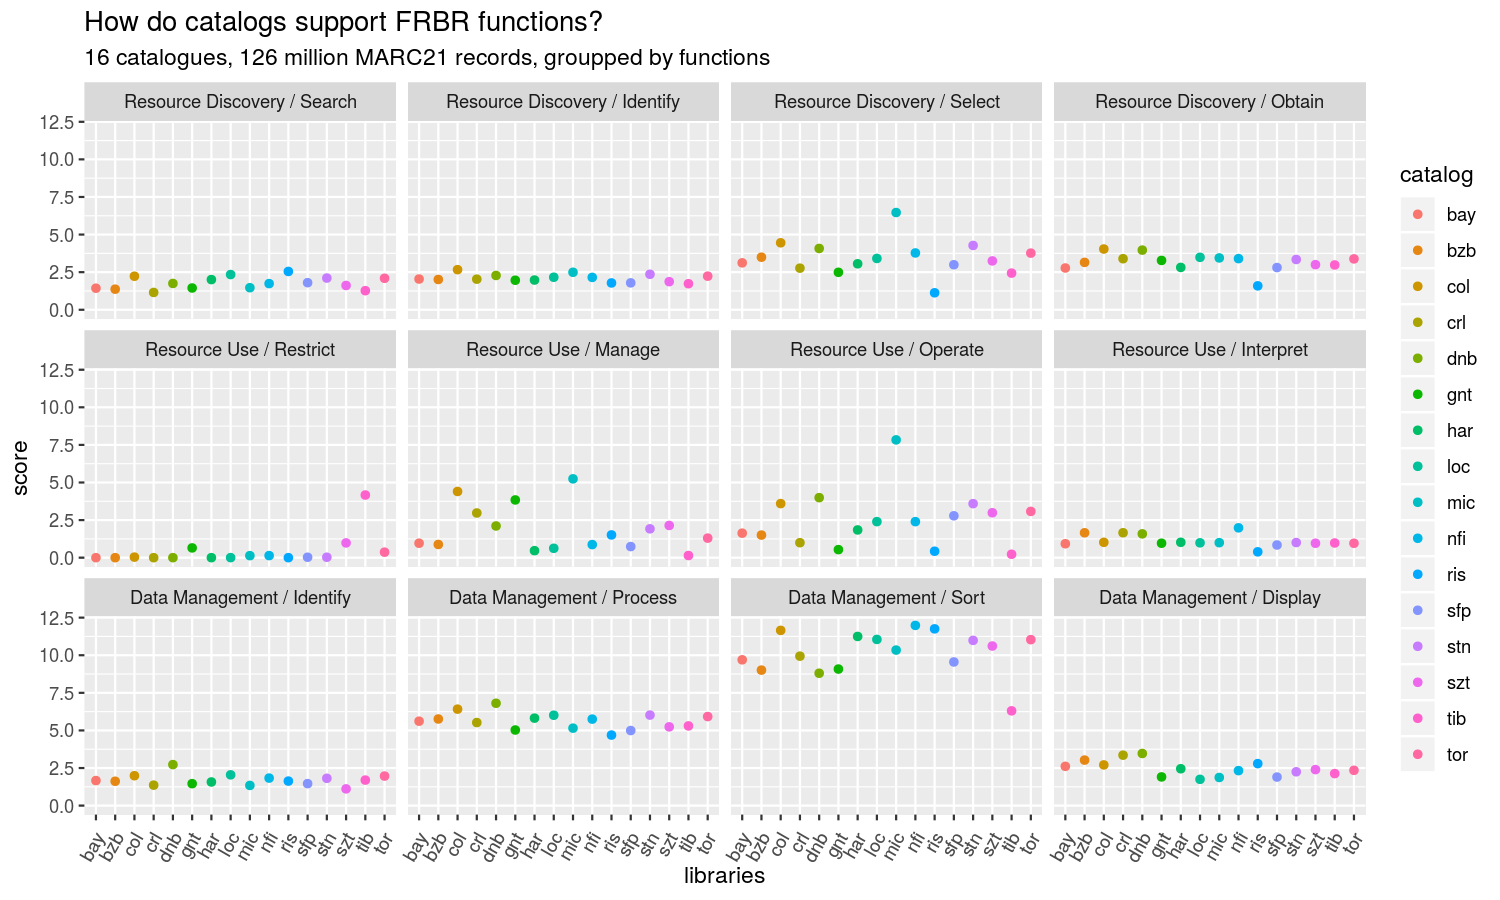
\includegraphics[width=\textwidth]{images/chapter04/functional-analysis-of-catalogs-by-catalogs.png}
\caption{Support of user tasks per catalogues I. Comparison per catalog}
\label{figure:functions-by-catalogs}
\end{figure}

\begin{figure}
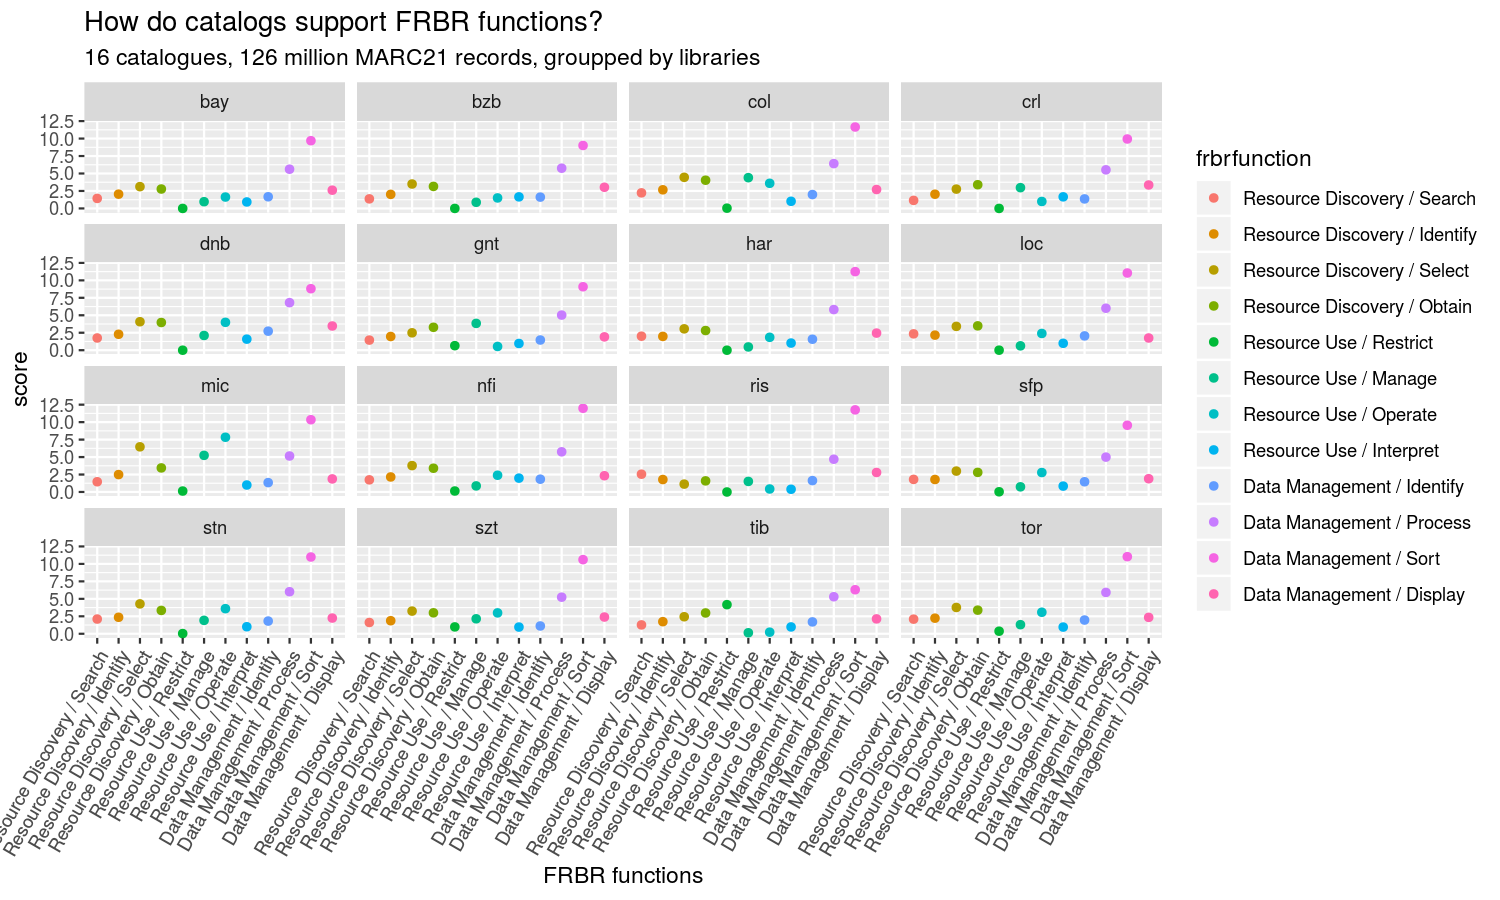
\includegraphics[width=\textwidth]{images/chapter04/functional-analysis-of-catalogs-by-functions.png}
\caption{Support of user tasks per catalogs II. Comparison per function}
\label{figure:functions-by-functions}
\end{figure}

\afterpage{%
    \clearpage% Flush earlier floats (otherwise order might not be correct)
    \thispagestyle{empty}% empty page style (?)
    \begin{landscape}% Landscape page
\begin{table*}
\caption{Support of user tasks (average score, scale: 0-100)}
\label{table:functional-analysis}
\hspace{-1cm}
\begin{minipage}{\columnwidth} %{\columnwidth}
\begin{center}
\begin{tabular}{lrrrrrrrrrrrrrrrr}
\toprule
function & bay & bzb & cer & col & dnb & gen & har & loc & mic & nfi & ris & sfp & sta & szt & tib & tor \\
\midrule
%\midrule
%\midrule
\multicolumn{17}{c}{Resource discovery} \\
%\midrule
Search & 1.4 & 1.4 & 2.2 & 1.2 & 1.7 & 1.4 & 2.0 & 2.3 & 1.5 & 1.7 & 2.5 & 1.8 & 2.1 & 1.6 & 1.3 & 2.1 \\
Identify & 1.6 & 1.5 & 2.3 & 1.8 & 1.7 & 1.7 & 1.7 & 1.9 & 1.4 & 1.8 & 2.0 & 1.6 & 1.9 & 1.5 & 1.3 & 1.8 \\
Select & 2.0 & 2.5 & 4.0 & 2.6 & 2.6 & 2.2 & 3.1 & 3.6 & 2.9 & 3.8 & 1.8 & 3.0 & 3.3 & 2.4 & 1.3 & 3.1 \\
Obtain & 2.1 & 2.3 & 3.4 & 3.0 & 3.1 & 2.9 & 2.3 & 3.1 & 1.8 & 2.9 & 1.9 & 2.4 & 2.5 & 2.3 & 2.3 & 2.7 \\
\multicolumn{17}{c}{Resource use} \\
Restrict & 0.0 & 0.0 & 0.0 & 0.0 & 0.0 & 0.6 & 0.0 & 0.0 & 0.1 & 0.1 & 0.0 & 0.0 & 0.0 & 1.0 & 4.2 & 0.4 \\
Manage & 0.6 & 0.6 & 5.9 & 5.0 & 1.0 & 6.5 & 0.8 & 0.9 & 2.4 & 1.1 & 2.6 & 0.9 & 1.2 & 1.8 & 0.1 & 0.9 \\
Operate & 2.1 & 2.0 & 6.8 & 3.1 & 4.5 & 1.6 & 5.8 & 7.2 & 8.3 & 6.3 & 1.4 & 6.4 & 5.5 & 5.0 & 0.0 & 4.5 \\
Interpret & 0.1 & 0.9 & 0.2 & 0.9 & 0.8 & 0.1 & 0.2 & 0.2 & 0.2 & 1.2 & 0.4 & 0.2 & 0.2 & 0.1 & 0.1 & 0.1 \\
\multicolumn{17}{c}{Data management} \\
Identify & 1.3 & 1.2 & 1.8 & 1.0 & 2.3 & 1.2 & 1.4 & 1.6 & 0.9 & 1.6 & 1.2 & 1.2 & 1.4 & 0.9 & 1.3 & 1.6 \\
Process & 2.0 & 2.2 & 2.8 & 1.9 & 3.2 & 1.6 & 2.2 & 2.4 & 1.6 & 2.2 & 1.9 & 2.0 & 2.4 & 1.7 & 1.7 & 2.3 \\
Sort & 9.7 & 9.0 & 11.7 & 9.9 & 8.8 & 9.1 & 11.3 & 11.1 & 10.3 & 12.0 & 11.8 & 9.6 & 11.0 & 10.6 & 6.3 & 11.0 \\
Display & 2.6 & 3.0 & 2.7 & 3.4 & 3.5 & 1.9 & 2.5 & 1.7 & 1.9 & 2.3 & 2.8 & 1.9 & 2.2 & 2.4 & 2.1 & 2.3 \\
\bottomrule
\end{tabular}
\end{center}
%\bigskip
%\footnotesize
%Note: The numbers in the columns represents the percentage of a given type for all issues in the catalog. Character `--' means that a given type does not occur in the catalog, while `0.0' means a percentage close to zero.
\end{minipage}
\end{table*}
    \end{landscape}
    \clearpage% Flush page
}

% \cite{thompson-traill2017}


\section{Future work}

MARC is an evolving standard, its new rules should be implemented in the newer versions of the software. MARC has a number of strict syntactic rules, but there are also semantic rules, which are not as easy to validate. Content wise there are external rule sets such as the ISBD \cite{isbd}, AACR2 \cite{aacr2} or RDA\footnote{http://rda-rsc.org/content/rda\_faq} which were not explored in this research. I would like to encourage the libraries to publish their local MARC element definitions and to update the software with these rules. A web based user interface with faceted search and data visualization is under construction\footnote{https://github.com/pkiraly/metadata-qa-marc-web}. Data science methods provide us with the possibility of deeper analysis. A Gent catalogue record has the following responsibility statement: ``Herr Seele (tekeningen); Toon Coussement (foto's); Peter Claes, Kris Coremans en Hera Van Sande, vakgroep architectuur en stedenbouw Universiteit Gent (vormgeving).'' The same record lists four authority entries: ``Herr Seele'', ``Coussement, Toon'', ``Claes, Peter'', and ``Van Sande, Hera'' while ``Kris Coremans'' is missing. A comparision of the authority entries and a list extracted by named entity detection would highlight the missing name.

\section{Note about reproducibility}

This research analyzed mostly freely available data sources. The download links, format, and license information of each are provided in section 3.2. The analysis software is an open source tool that is available under the GPL-3.0 license. The binary versions are distributed via Maven Central, a repository for Java libraries. The software is properly documented, and provides helper scripts. Continuous integration (via Travis CI) and automatically generated transparent code coverage reports help to maintain the quality of the software. For every research software project it is a crucial point whether the tool could escape the confines of the laboratory walls. The author is happy to cooperate with libraries to improve the software, and thus the quality of the catalogues. The generated reports behind Table \ref{table:proportion-of-issues} and \ref{table:issue-types} are available as supplemental materials\footnote{https://doi.org/10.25625/AMF8JC}.

\section{Acknowledgement}
Thanks for Johann Rolschewski and Phú for their help in collecting the list of published library catalog, Jakob Voß for the Avram specification and for his help in exporting MARC schema to Avram, Carsten Klee for the MARCspec. I would like to thank the early users of the software, Patrick Hochstenbach (Gent), Osma Suominen and Tuomo Virolainen (FNL), Kokas Károly and Bernátsky László (SZTE), Sören Auer and Berrit Genat (TIB), Shelley Doljack, Darsi L Rueda, and Philip E. Schreur (Stanford), Marian Lefferts (CERL), Alex Jahnke and Maike Kittelmann (SUB) who provided data, suggestions or other kinds of feedback, Justin Christoffersen for language assistance. Special thanks to Reinhold Heuvelmann (DNB) for terminological and language suggestions.

% \bibliographystyle{acm}
% \bibliography{bibliography-for-papers}

\chapter[Towards an extensible measurement of metadata quality]{Towards an extensible measurement of metadata quality\footnote{This chapter is an extended version of the paper \cite{kiraly2017}.}}

\section{Introduction}

In the literature about metadata quality measurement\footnote{The most current bibliography of the topic is the collaborative Metadata Assesment Zotero group library created by the DLF AIG Metadata Working Group (\url{http://dlfmetadataassessment.github.io/}). Available at \url{https://www.zotero.org/groups/metadata_assessment}.} it is rare that the authors give any hint about their implementation methods or give a reference to their source codes. 
Thus --- since we lack the opportunity of studying the implementation details ---, we are forced to assume that these projects aimed to measure one specific dataset based on a particular metadata schema. When we started our research, it was an important aspect that the tool we design (called Metadata Quality Assurance Framework\footnote{Background information, documentation and source codes are available from \url{http://pkiraly.github.io/}.}) should work together with different metadata schemas and formats.

The quality assessment process has three phases:

\begin{enumerate}
\item Measuring individual metadata records
\item Analyzing the results with statistical methods to get metrics of the dataset
\item Reporting results
\end{enumerate}

The results of the first phase are table-like data structures containing mostly numerical values. Since these type of results are very similar for different metadata schemas, the second phase can already be handled in general way with statistical and data science methods. We should however investigate the first step further. The basic process of measuring is the following: we take a record as a formatted string (in JSON or XML format), address individual parts to check their existence, cardinality or other properties such as different features of their content and return the results of these checks (typically in numerical form). If we want to like to abstract this process we should figure it out how to list and access individual parts of the metadata record, and we also should provide schema independent measurement methods.

This paper will describe the steps we took so far to support this abstraction, which enables us to measure different metadata collections with a single tool.

\section{Types of measurement}

The main types of data quality measurement we can run on metadata records are the following:

1. General structural and semantic metrics. These measurements are the most well known in the literature, and following the seminal articles \cite{bruce-hillmann2004, ochoa-duval2009} several projects reported to measure
the metrics of completeness (the existence of the defined fields in the records), accuracy (comparison of a full data object and its metadata), conformance to expectations (schema rule validation and information value), logical consistency and coherence, accessibility (how easy is to understand the text of the record), timeliness (the metadata quality change over time) and provenance (the relationship between other metrics and the creator of the data).

2. Support of functional requirements. Each data schema is created for supporting a set of functionalities, such as searching, identifying or describing objects. The data elements support one or more of these functionalities, and their existence and content has an impact of these functionalities. An example: a timeline widget expects a specific date format; if the field value is in another format the widget will ignore it. This family of metrics gives measures the scale of support of the functional requirement. To apply these metrics we should take the functional requirement analysis of the data schema and map the individual data elements (classes and properties) to the functionalities. The result will be a report which tells how the data support the intended functions. Following the terminology established in \cite{gavrilis2015} we call these scores `sub-dimensions'. In the Europeana Data Quality Committee Valentine Charles and Cecile Devarenne defined a number of sub-dimensions (such as searchability, descriptiveness, identification, contextualization, browsing etc.) which could be re-used in other metadata domains.

3. Existence of known data patterns. These are schema- and domain-specific patterns which occurs frequently in the datasets. There are good patterns which detect good data creation practices, and anti-patterns, which should be avoided (such as data repetition, meaningless data etc.). For some domains there are existing pattern catalogs (e.g. the Europeana Data Quality Committee works on a Europeana specific pattern catalog, while \cite{suominen2012} examined three SKOS validation criteria catalogs).

4. Multilinguality. RDF provides an easily adaptable technique to add a language tag to literal values, and multilinguality has become a key aspect in the Linked Open Data world. In cultural heritage databases the translation of the descriptive fields (such as title, description) might be quite a resource-intensive task. On the other hand reusing existing multilingual dictionaries for subject headings is a relatively simple and cheap process. On the measurement side the nice thing is that generally the multilingual layer in metadata schemas (even in those not built on top of RDF) are similar, so the implementation can be abstracted. The big problem is how to handle the biases generated by the different cardinality and importance of the data elements. Imagine that we have a subject heading which is accessible in several language, but it is attached to a great portion of records, so its information value or distinctive power is low. See more about multilinguality in \cite{stiller-kiraly2017}.

The common point in these metrics is that they can be implemented as generic functions where input parameters are specific elements of a data schema. The functions themselves should not know about the details of the schema; that is to say they should be schema-independent. In other words: the only thing we should need to create on a schema by schema basis is a method which takes care of mapping the schema elements and measurement functions and feeds these generic functions with the appropriate metadata elements.

Note: based on these metrics in the following, analytical phase we have to create a mathematical model that generates one or more top level data quality score for the record; this article does not discuss this phase.

\section{Mapping schema and measurements}

A metadata schema describes the structure of the record, and optionally gives us constraints upon the values of the fields. In order to measure the metadata quality we need various pieces of information about the schema:

\begin{itemize}
 \setlength{\parskip}{0pt}
 \setlength{\itemsep}{0pt plus 1pt}
\item What are the fields we would like to analyze?
\item Are there any special properties of a field (e.g. mandatory or optional, repeatable, content-related constraints, special format)?
\item Are there fields we have to extract to identify the record or a subset of the collection?
\item Are there field groups which can behave in special way? (For example: if a record must have at least a title or an alternative title, we should group these together, and when we check the mandatory elements we should return true if at least one element of the group exists. Conversely, disjoint fields (which are mutually exclusive) should be checked that only one one of them is available in the record, but never more.)
\end{itemize}

In the previous section we mentioned that we have to create a mapping mechanism which dispatches the elements of the metadata record to different measurement functions. In the first iteration of the Metadata Quality Assurance Framework we have created an abstract concept of the schema, which lists the metadata elements needed for the quality analyses. Each element has a name, an address with which we can find its occurrence in the record, and different properties which denote its role in a particular function (for example the list of sub-dimensions it is part of, the list of field groups, whether it might have language annotation etc.). The mapping supports parent-children relationship, so the functions can recurse down the hierarchy.

A prerequisite for measuring information value is a searchable index, which we implemented with Apache Solr. In our framework, metadata fields are accordingly mapped to Solr field names.

In this mapping we record all information about the metadata schema which is necessary for the measuring. At time of writing the manifestation of this mapping is a Java class.\footnote{Such as \url{https://github.com/pkiraly/metadata-qa-api/blob/master/src/main/java/de/gwdg/metadataqa/api/schema/EdmOaiPmhXmlSchema.java}} To run the measurement on a new schema, one should create first this mapping object. In the future we will create user friendly interfaces (web-based editorial form and XML/RDF annotations) which are more familiar tools for the intended audience, the community of metadata experts.

\subsection{Addressing elements}

An important part of schema handling is how we address the particular parts of the record. In the XML world XPath\footnote{XML Path Language (XPath). Version 1.0. W3C Recommendation 16 November 1999 (Status updated October 2016). \url{https://www.w3.org/TR/xpath/}} provides with a standard way to solve this problem. The current version of the Metadata Quality Assurance Framework (version 0.4) supports only JSON records, so we make use of a similar tool, JsonPath\footnote{Stefan Goessner: JSONPath --- XPath for JSON. \url{http://goessner.net/articles/JsonPath/}. Actually we make use its Java port, the Jayway JsonPath available at \url{https://github.com/jayway/JsonPath}} which has a different syntax, but offers the same functionality. To illustrate it here is an example for the Europeana Data Model (EDM) metadata schema\footnote{The Europeana Data Model Documentation is available at \url{http://pro.europeana.eu/share-your-data/data-guidelines/edm-documentation}}:

\begin{lstlisting}[caption=A JSON path example]
$.['ore:Proxy']
  [?(@['edm:europeanaProxy'][0] == 'false')]
  ['dc:title']
\end{lstlisting}

This expression addresses the dc$:$title field instances of the ore$:$Proxy part in which the value of the first edm$:$europeanaProxy instance is 'false'.

\begin{lstlisting}[caption=An excerpt of an EDM metadata record]
{
  "ore:Proxy": [
    {
      "edm:europeanaProxy": ["false"],
      "dc:title": [
        {
          "@lang": "de",
          "#value": "Pyrker-Oberwart, Johann Ladislaus"
        }
      ],
      ...
    },
    {
      "edm:europeanaProxy": ["true"],
      ...
    }
  ]
}
\end{lstlisting}

Here you can see that the ore$:$Proxy is a list of two objects. The first one's edm$:$europeanaProxy is 'falue', the second one's is 'true'. Since we are looking for the the object with the 'false' value, we get the first. It has a 'dc$:$title' property. The return value will be the Java representation of the following JSON string:

\begin{lstlisting}[caption=The selected part of the record]
[
  {
    "@lang": "de",
    "#value": "Pyrker-Oberwart, Johann Ladislaus"
  }
]
\end{lstlisting}

In this example we showed an absolute path, which searches from the root of the record, but since the schema abstraction supports parent-child relations, we can use relative paths as well.

\subsection{Flexible and configurable measurements}

\subsubsection{The overall picture}

The system's central entry point is the CalculatorFacade (or its extension). It provides us with a number of configuration options. The most important one is the registration of the schema mapping. Based on the settingsin the schema mapping it prepares the measurement classes for running. When it is ready to run the process passes every record to the measure() method. It accepts the metadata record as a JSON string, runs all the measurements which have been configured, and returns a CSV representation of the result of the metrics. As indicated by the name it is just a Facade object\footnote{See \url{https://en.wikipedia.org/wiki/Facade_pattern}}: it only coordinates the process, the actual measurements are done by the individual 'calculators' (the generic schema-agnostic functions we mentioned above). These all implement the Calculator interface, and they have three important methods. The 'measure()' method accepts a cacheable representation of the metadata record and performs the measurement. The 'getCsv()' method returns the result of the measurement, while 'getHeader()' method returns a list of the column names for the CSV row. The cacheable representation is a special object. It contains the full record or a part thereof, applies the JsonPath expressions, and transforms the resulting object into a uniform Java object, which provides a simplified DOM-like interface. In this fashion the Calculators can access the values in a generalized way, and can reuse the already-processed parts from the cache. Retrieving the parts of the record is computationally expensive: one part might participate in multiple measurements, but this way we have to retrieve it only once.

Each calculator implements one or more metrics. Since at run-time (in the measuring phase) they can not get extra arguments, if a calculator has conditional steps depending on properties which are not part of the schema, they should be configured ahead of the measuring phase via the CalculatorFacade's 'configure()' method. For example the 'MultilingualitySaturationCalculator' can emit its results in either simple and complex form, depending on the 'resultType' setting. The client should decide the format before running the measurement, and set the appropriate one in the Facade class.

This way the CalculatorFacade are extensible, and one can write additional Calculators. The tool currently provides all Calculators required for our current research.

\subsubsection{Metadata problem patterns}

Problem patterns are known issues in the metadata record instances. In case of Europeana Timothy Hill and Hugo Manguinhas have led the initiative to collect all those problems\footnote{Data Quality Committee: Problem Patterns. Available at \url{http://bit.ly/2jIXQGU}}. They categorized the problems into several types, such as duplicate or redundant information, irrelevant information (such as non-meaningful titles, e.g. "unknown title"), missing or incomplete information, misuse of fields, just to name a few.

The current implementation of the problem catalog measurement has been done based on the Observer design pattern \footnote{\url{https://en.wikipedia.org/wiki/Observer_pattern}}. There is a central class --- ProblemCatalog\footnote{\url{https://github.com/pkiraly/metadata-qa-api/blob/master/src/main/java/de/gwdg/metadataqa/api/problemcatalog/ProblemCatalog.java}} --- which implements the Calculator interface, so it has a 'measure()' method. This class acts as the observable subject, and it notifies its subscribers (the observers) when they have to measure a new record. Each individual problem is associated with a distinct class (a ProblemDetector\footnote{See for example the 'EmptyStrings' class which detects empty strings in field instances: \url{https://github.com/pkiraly/metadata-qa-api/blob/master/src/main/java/de/gwdg/metadataqa/api/problemcatalog/EmptyStrings.java}}), which implements the Observer interface, and accordingly has a method called 'update()'. It has two parameters: the metadata record, and a variable which is a collector of the measurement results. In this case the result should be a number: how many times the pattern occurs in the record. When the measure is started, the ProblemCatalog class creates a collector for these results, and the client (the facade class) will retrieve it when the measurement is done.

The ProblemCatalog class has 'addObserver()' method to register the subscribers, which should be done at the central facade class at configuration time.

For detecting new problems one has to create new ProblemDetectors and register them in the central CalculatorFacade.

\subsection{Extensions and APIs}

The current Java APIs are defined in a core library (metadata-qa-api) which contains the workflow governing mechanism, and the general schema-agnostic functionalities. There is an extension of this API, called 'europeana-qa-api' that contains the Europeana-specific measurement and facade. These libraries are published in the central Maven repository\footnote{\url{http://mvnrepository.com/artifact/de.gwdg.metadataqa}}, so any further extension can add these into its dependency tree in the local Maven configuration file (pom.xml) as

\begin{lstlisting}[caption=Including the Java libraries into other project]
<dependencies>
  <dependency>
    <groupId>de.gwdg.metadataqa</groupId>
    <artifactId>metadata-qa-api</artifactId>
    <version>0.4</version>
  </dependency>
  <dependency>
    <groupId>de.gwdg.metadataqa</groupId>
    <artifactId>europeana-qa-api</artifactId>
    <version>0.4</version>
  </dependency>
  ...
</dependencies>
\end{lstlisting}

We have created two clients for the Java APIs: the first enables measurement with the popular Big Data analytics tool Apache Spark; the second one provides us with a REST interface.

\subsubsection{Big Data analysis}

Apache Spark is an extremely efficient tool for batch processing of huge datasets (the Europeana dataset is more than 400 GB). Combined with Apache Hadoop's distributed file system it can be run either on a single machine or in a distributed computing environment. The users can specify the details of allowable resource usage (number of CPUs, memory usage, etc.) and it comes with a web based monitoring tool. In the file-based workflow, Spark reads and processes lines one by one; it requires us to store one record per line (however Spark also supports different other data sources such as NoSQL databases, where this constraint does not exist). In our Spark based client the result is stored as CSV files.

\subsubsection{Data analysis with REST APIs}

The REST interface provides two kinds of API: a simple Record API, which runs the measurement on individual records and returns a CSV or JSON response, and another one which is called Workflow API and enables a full measurement workflow.

\begin{lstlisting}[
  % one can adjust spacing here if required
  % aboveskip=2.5\baselineskip,
  % belowskip=-.8\baselineskip,
  caption={Quality measurement of a single record REST API response},
  label=code:single-record-api-json-response,
  language=Bash,
  float]
GET /07602/696BE60475DFAF290B7CD7759E840CD4FFF86E24.json

{
  "existingFields":[
    "edm:ProvidedCHO/@about", "Proxy/dc:title", "Proxy/dc:creator",
    "Proxy/dc:publisher", "Proxy/dc:type", "Proxy/dcterms:spatial",
    ...
  ]
  "emptyFields":[],
  "labelledResults":{
    "fields":{
      "recordId":"/07602/696BE60475DFAF290B7CD7759E840CD4FFF86E24",
      "dataset":"07602_Ag_IT_Culturalitalia_RegioneMarche",
      "dataProvider":"Regione Marche / SchedeS:AN" },
      "completeness":{
        "TOTAL":0.542857, "MANDATORY":1.0, "DESCRIPTIVENESS":0.454545,
        ...
      },
      "existence":{
        "edm:ProvidedCHO/@about":true, "Proxy/dc:title":true,
        "Proxy/dcterms:alternative":false, "Proxy/dc:description":false,
        ...
      },
      "cardinality":{
        "edm:ProvidedCHO/@about":1, "Proxy/dc:title":1,
        "Proxy/dcterms:alternative":0, "Proxy/dc:description":0,
        ...
      },
      "uniqueness":{
        "dc:title:sum":0.001084, "dc:title:avg":1.807687E-4,
        "dcterms:alternative:sum":0.0, "dcterms:alternative:avg":0.0,
        "dc:description:sum":0.0, "dc:description:avg":0.0
      },
      "problemCatalog":{
        "LongSubject":1.0, "TitleAndDescriptionAreSame":0.0,
        "EmptyStrings":0.0
      },
      "languages":{
        "Proxy/dc:title":{ "_0":1 }, 
        "Proxy/dcterms:alternative":{ "_1":1 },
        ...
      }
    },
    "termsCollection":{
      "dc:title":[
        {"term":"ancona", "tf":1, "df":12388, "tfIdf":8.072328-5},
        {"term":"carta", "tf":1, "df":87048, "tfIdf":1.148791-5},
        ...
      ],
      "dcterms:alternative":[],
      "dc:description":[]
    }
  }
}
\end{lstlisting}

Listing \ref{code:single-record-api-json-response} shows a formatted representation of the Record API call. It accepts two parameters, the record ID, and the format (either as JSON or CSV) as file extension. The result contains all the measurement results for an individual record. At time of writing the measurements are existence, cardinality, uniqueness, problem catalog and languages. The languages part contains pairs of languages and their count for each fields. There are three special codes to encode cases where there is no language annotation:

\begin{itemize}
  \setlength{\parskip}{0pt}
  \setlength{\itemsep}{0pt plus 1pt}
  \item \_0: no language tag specified
  \item \_1: the field is missing (the very same information that of field existence metric)
  \item \_2: the field is a resource (it contains a URL or tagged as resource)
\end{itemize}

The user interface's record level display is based on the Record API.

\begin{figure}
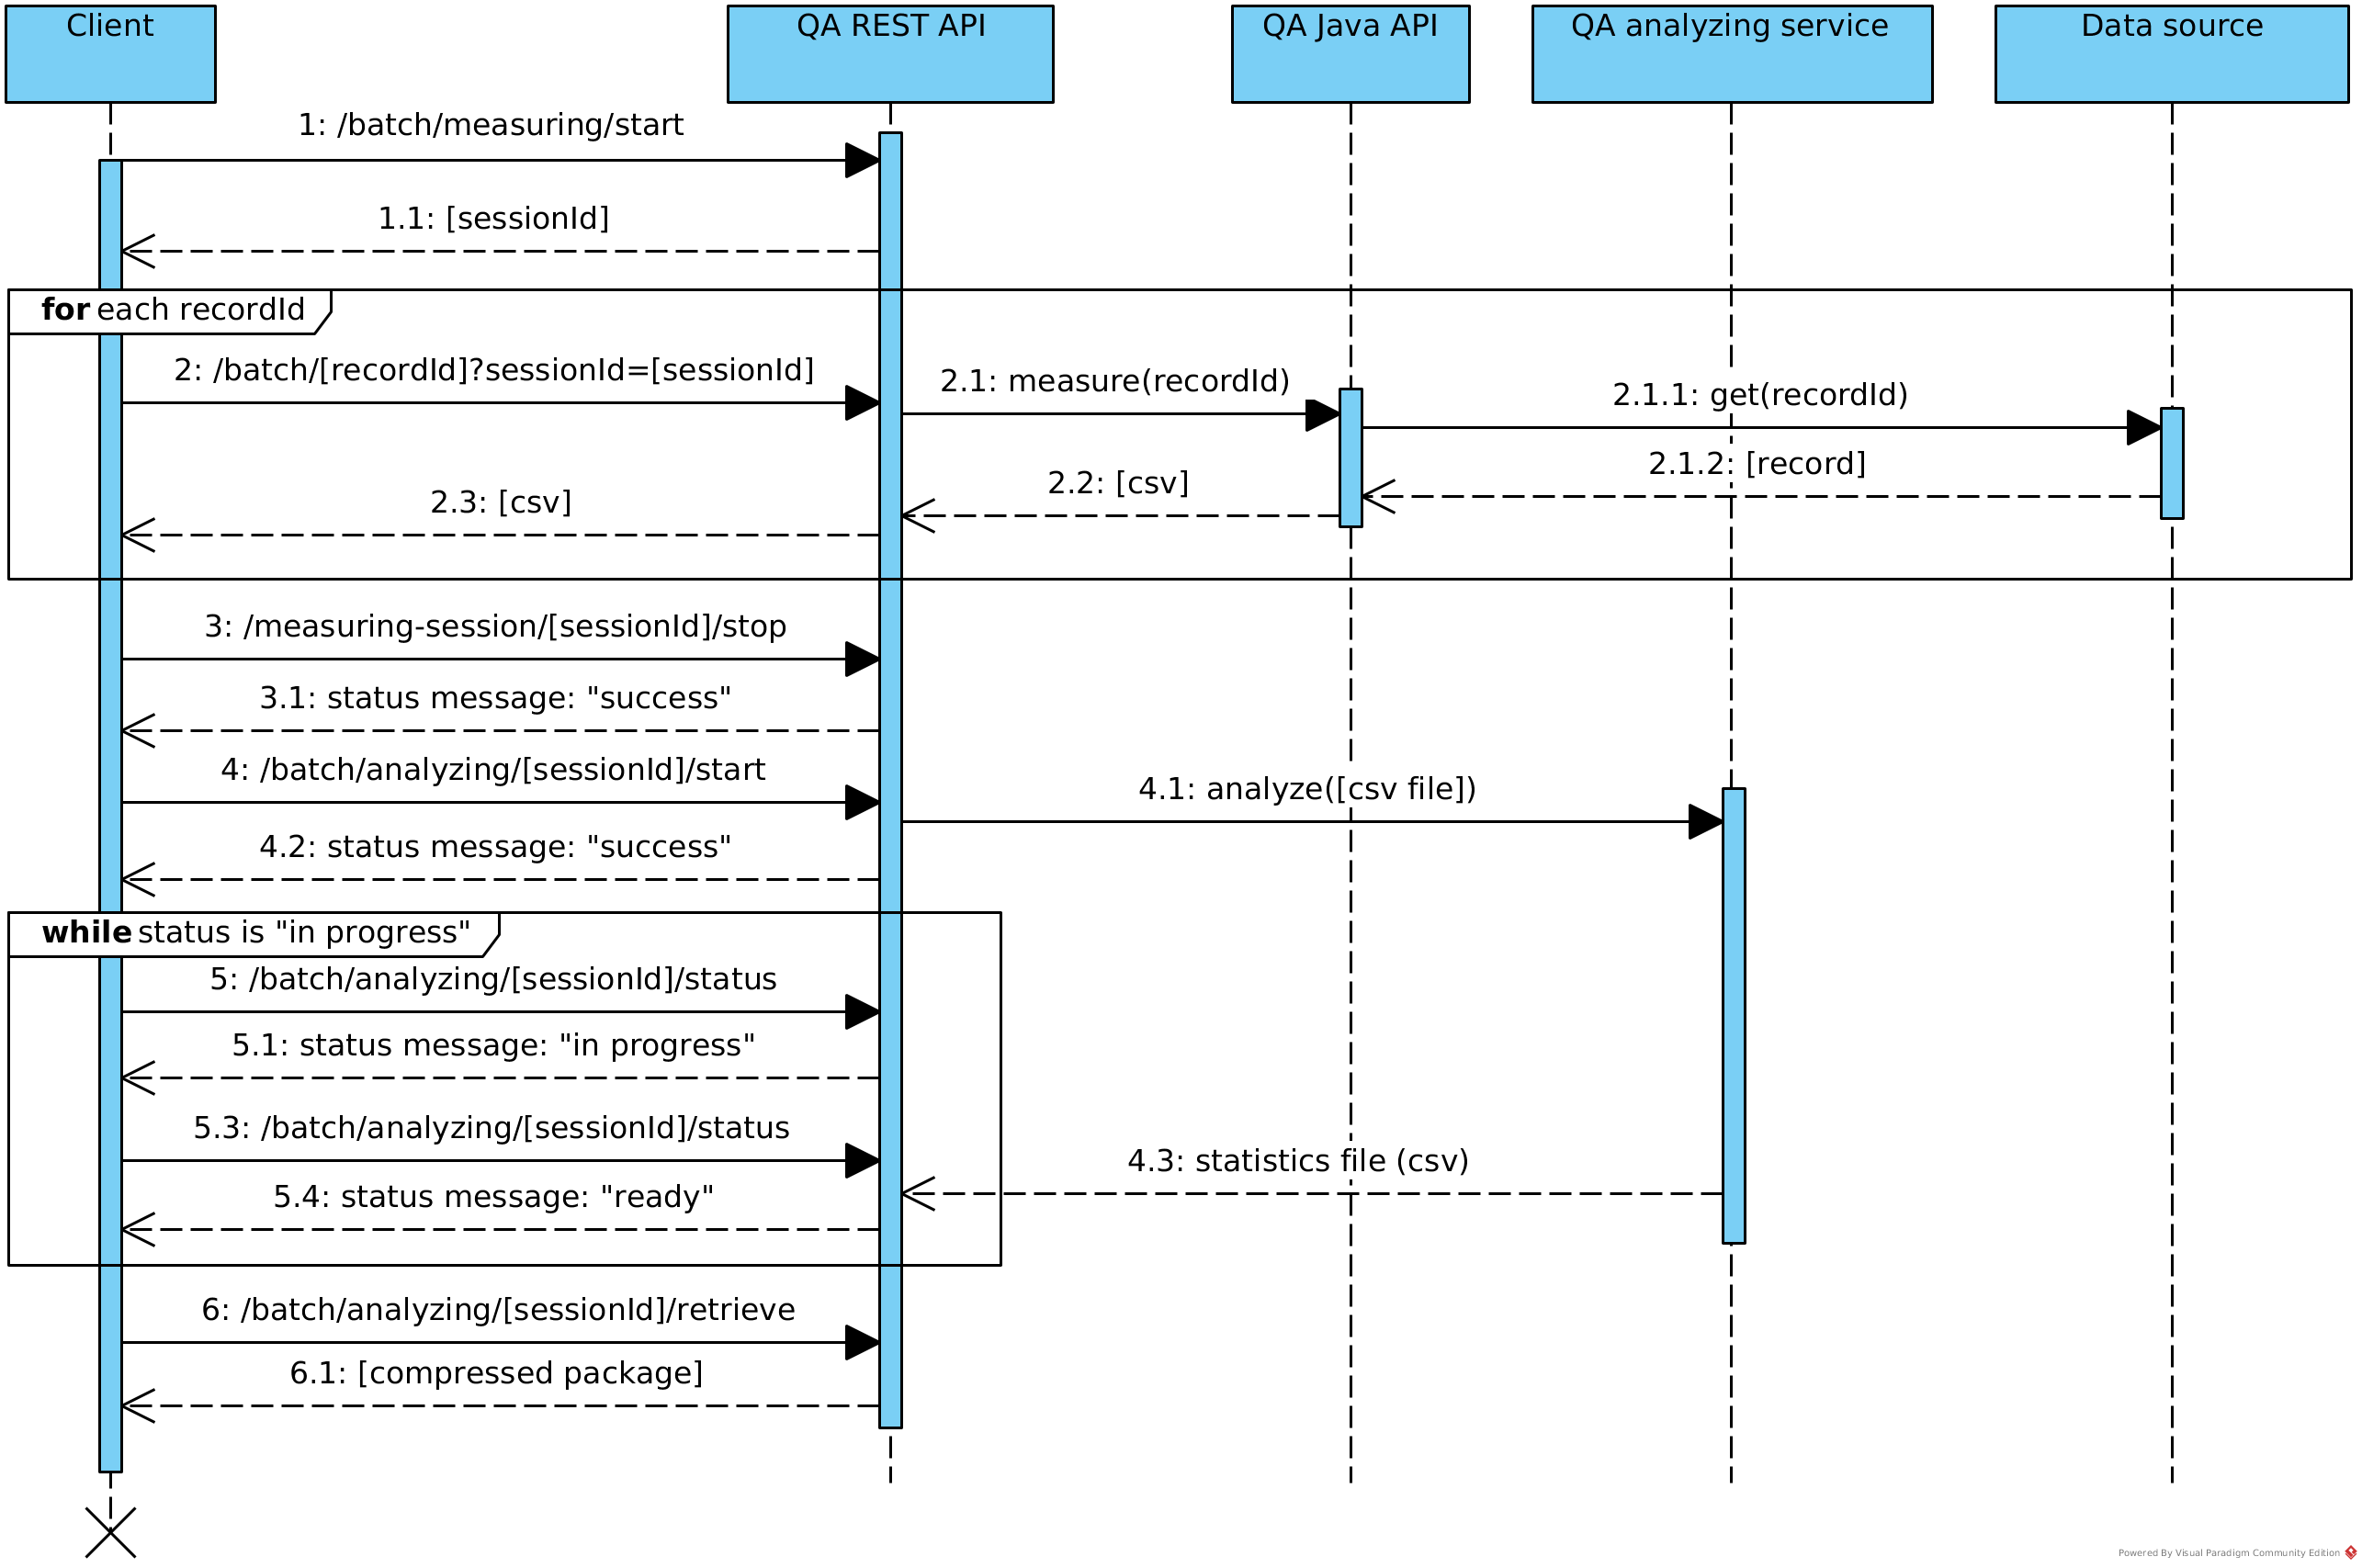
\includegraphics[width=\textwidth]{images/chapter05/QA-REST-API-interactions.png}
\caption{Processing time per records with different settings}
\label{fig:workflow-api}
\end{figure}

The Workflow API supports the whole life cycle of the metadata quality measurement process, so it measures individual records, then analyze them by running statistical functions on aggregated metrics. The full workflow is depicted by Figure \ref{fig:workflow-api}. 

First, the client initializes a session, to which the server returns a session identifier which should be used during the whole workflow. Then client submits record IDs one by one. The server is responsible for storing the results in a CSV file, but it also returns a CSV row for each record call, same way as the Record API does. Once all records were measured, the client stops the measuring part, and starts the analysis part, in which the server calls the external analyzer (either a R script or a Spark based analysis process) to produce a report containing the result of the statistical analysis and (optionally) generated images files. This process is time consuming, and the client can repeatedly ask for the status of the process. The server reports if the process is ``in progress'' or ``ready''. When it is finished, the client can retrieve the result as a zipped package. This process is very useful if the client would like to check only a part of the whole collection. Combined with other tools (e.g. with a search API) it is possible to select the IDs of a subset -- for example the newly ingested records, or a specific result set.

The main reason for creating REST APIs is that this way the back end functionalities of the framework became interoperable: the metrics could be reused in the client's own existing systems.

\section{Conclusions and future works}

In this paper we showed the most important technical requirements of an extensible metadata quality assessment framework. We discussed the first phase of the metadata quality analytics workflow only, the measurement part. It can ingests different metadata schemas, but emits numerical, tabular data in a standardised form. The statistical analysis, and the reporting based on this, and do not require the same abstracting approach as the first step.

We showed the main characteristics of the metadata quality metrics and the metadata schema, then how to map schema features to measurement functions and how to address internal parts of a metadata record. We discussed the relevant design decisions of our implementation, and highlighted the parts which should be extended if one adapts the method for another metadata schema. Finally we described the APIs of the system.

By the time of writing no other projects started to use this framework, so we do not have real external feedback about the flexibility of the framework. Our own experiments were based on two metadata schema: Europeana Data Model (EDM) and MAchine Readable Catalog (MARC21) --- both of which have relatively simple structures. We expects that every new metadata schema will raise at least some new requirements, and only after having successfully dealt with a variety of schemas will we be in a position to release a 1.0 version of the tool. The level of schema abstraction is adequate for current purposes, but we anticipate the addition of several new features in the future. We are constantly looking for collaborating partners to try this approach on new schemas and in different IT environments. Starting and continuing discussions with organizations having similar approaches and requirements in the realms of digital libraries, the semantic web, digital humanities, and learning objects, and learning from each other will be a crucial aspect of creating a truly interoperable framework.

\section{Acknowledgments}
We would like to thank Europeana and GWDG for providing computational environment for this research. For this research Cecile Devarenne and Yorgos Mamakis (Europeana) for giving suggestions regarding to the Workflow API, and all the members of the Data Quality Committee\footnote{\url{http://pro.europeana.eu/page/data-quality-committee}} for their work, and Timothy Hill for language-related suggestions.

% \bibliographystyle{acm}
% \bibliography{bibliography-for-papers}

\chapter{Predicting optimal Spark settings in standalone mode}

\emph{Abtsract} What are the optimal parameter settings for a long running, standalone mode Spark based, stateless process? The chapter investigates the effects of four different parameters and compares the application's behaviour in two different servers. Two important lessons learned from this experiment are: i) allocating more resources does not necessary imply better performance, ii) creating an environment with limited and shared resources -- which politely let other processes run -- is a `good enough' state. To discover the optimal settings it is suggested to pick up a smaller sample that shares important features with the full dataset, and measure their performance against different settings. The settings to check are: number of cores, memory allocation, compression of the source files, and reading data from different file systems (if they are available). As a source of ground truth default Spark processing log, Spark event log, or measuring points inside the application can be used.

%\keywords{Apache Spark \and performance metrics \and metadata quality \and Europeana.}

\section{Introduction}
Measuring the quality of cultural heritage metadata is a task which has two important features. First, in Digital Humanities (DH) context the size of source data (library, archives or museum (LAM) catalogues, or aggregated catalogues/datasets such as Europeana\footnote{\url{https://europeana.eu}}, Wikidata\footnote{\url{https://wikidata.org}} or Archives Portal Europe\footnote{\url{http://www.archivesportaleurope.net/}}) could be regarded as big data. Big Data is a relative concept, usually it means that the data is larger than what you could process with traditional methods within the infrastructure available in the organization. DH or even cultural heritage traditionally is not equipped with high performance computing tools, so here the volume of Big Data are smaller than for example in astrophysics, or medicine. On the other hand the variety of the data is large. Second, even after a decade of research (\cite{zotero-bibliography}), the LAM community has not yet reach a clear consensus on the exact meaning of metadata quality. We have different quality dimensions and metrics, but current researches are still experimental and in some extent based on trial and error workflow, in which metrics are selected from the literature or new metrics are invented, their measurements are implemented and tried on the (meta)data, finally metadata experts evaluate the result, and suggest changes on the measurement. The consequence of this research cycle is that it necessitates the execution of multiple long running measurements of the same big data set. Among other tools Apache Spark\footnote{\url{http://spark.apache.org/}} helps to decrease the duration of this process by letting the existing process run parallel fashion. Spark could be run in a cluster, but in a DH/LAM context clusters are rarely available, so a more typical use is to run Spark in `standalone mode' which make use the multicore architecture of a single machine and simplifies writing multithreaded software code. Commercial or scientific conference presentations about Spark performance usually concentrate on clustered environment, and one can hardly find suggestions on the standalone mode. This paper aims to suggest some easy preliminary measurement of a Spark run to find the optimal settings.

\section{Measuring completeness of Europeana records}
Europeana is a digital platform of the European cultural heritage, which aggregates catalog records from European libraries, archives, museums, and other cultural organizations (called data providers). In this research a snapshot of records were used which were created in 2018 August and contains approx. 62 million records. Each record are in Europeana Data Model (EDM)\footnote{\url{https://pro.europeana.eu/resources/standardization-tools/edm-documentation}} metadata schema, which has the several parts or `entities': a descriptive metadata part (`proxy'), and optional contextual entities which describe the agents, concepts, places and time spans mentioned in the proxy. Moreover Europeana not just aggregates these records, it enhances them as well: with the help of semantic web technologies and linked open data it tries to detect entities in the data provider's proxy, and to save them as additional contextual entities.

The data are stored in a MongoDB database. Since reading from MongoDB is time consuming process, and Spark's Mongo connector does not support a specific reference type which is heavily used in the database, we chose to export the data to text files in which every line is an individual, denormalized record (here denormalization means that the record packages together the proxies, and all linked contextual entities instead of merely keeping the references to them). The process is built on Spark's Mongo connector enhancing with some extra API calls\footnote{\url{https://github.com/pkiraly/europeana-qa-spark}}. The best part of Spark's Mongo connector, that like in the processing of text-based input files Spark makes partitions of Mongo, and able to run exporting them parallely. At the end of the process 1740 files each with 35.6 thousand records were created. The size of the files varies, their average size is 0.47 GB (the bulk is between 0.23 and 0.9 GB).

After this preparation phase comes a record level measuring part, which is based on Spark's Java API. In the project there are multiple measurements, for this experiment the \emph{completeness measurement} were selected. It takes a JSON string and checks every field in the schema whether they are available in the record and returns an integer (zero or more) denoting the number of available field instances. The result is serialized as a CSV formatted string which contains record identifiers, some selected metadata (the identifiers of sources of the records), and the fields cardinalities. Spark takes care of reading the input and writing the output, and distribution of the processing over the available CPUs. The part of the process which interacts with Spark is provided in Listing \ref{code:spark_api_usage}. The next steps are statistical analyses of the resulted CSV, which produce a set of CSV files with statistical description of the whole collection and its 20K subcollections (records belonging to the same dataset, data provider or provider, or records come from the same countries, or written in the same language -- and the combination of these), an their visualization on a web based user interface.

From Spark's perspective it is the most minimalistic use of Spark: above the mandatory input and output calls only one extra method is used: map(). It is important to know, that Spark API is similar to SQL queries that it is high level API, and the engine behind optimizes it and creates a low level implementation. When Spark starts it analyses the input to calculate the number of `tasks'. Each task takes an input, runs the code, and saves the output. Outside of the core processing Spark runs a monitoring web server, which is started before the first file read, and shut down after the last output. Spark also runs some file managing process in the background when merging and renaming output. The final output will be a list of files, and we have to merge them into a single file outside of the Spark process.

\begin{lstlisting}[
  % one can adjust spacing here if required
  % aboveskip=2.5\baselineskip,
  % belowskip=-.8\baselineskip,
  caption={The part of Java client code which interacts with Spark API},
  label=code:spark_api_usage,
  language=Java,
  float]
// initialize Spark
SparkConf conf = new SparkConf().setAppName("CompletenessCount");
JavaSparkContext context = new JavaSparkContext(conf);

// initialize the processing class
final EdmCalculatorFacade facade = ... 

// read input file
JavaRDD<String> inputFile = context.textFile(parameters.getInputFileName());

// definition of a method which process a lines
Function<String, String> baseCounts = new Function<String, String>() {
  @Override
  public String call(String jsonString) throws Exception {
    String result = "";
    try {
      result = facade.measure(jsonString);
    } catch (InvalidJsonException e) {
      // error reporting
    }
    return result;
  }
};

// processing every lines of input files
JavaRDD<String> baseCountsRDD = inputFile.map(baseCounts);

// save result
baseCountsRDD.saveAsTextFile(parameters.getOutputFileName());
\end{lstlisting}

\section{Tuning Spark and measuring performance}

There are several settings in standalone Spark process which worth playing with:
\begin{itemize}
 \setlength{\parskip}{0pt}
 \setlength{\itemsep}{0pt plus 1pt}
 \item number of cores
 \item memory allocation
 \item for file inputs:
 \begin{itemize}
  \setlength{\parskip}{0pt}
  \setlength{\itemsep}{0pt plus 1pt}
  \item whether they are stored in the operation system's file system, or in a Hadoop File System
  \item whether they are compressed of not
 \end{itemize}
\end{itemize}

We run the same measurement on two different machines on two input sets. The fist input set is the full corpus, while the second contains only ten files. The size of these files are also smaller (mean is 0.3 GB, while it is 0.47 GB for the full set). The first machine (`europeana') has a 2.4 times faster CPU then the second one (`roedel'). `Europeana' has 8 cores, `roedel' has 16 cores. The data, and the processing code were identical, as well as Spark version (2.4.0).

In this experiment the measured numbers are recorded in different sources. Spark log provides information about `stage' and `job' duration (in Spark processing hierarchy the process might have been split into multiple jobs, each having multiple stages -- in our case there is only one job with one stage). The process is launched by a bash script, which also measures the overall duration. Spark has a special event log (see later), which provides other important metrics, such as executors' run-time and CPU-time. Finally we put a time counter into the client source code, to record an important information: how much time does the map() function take (see Listing \ref{code:spark_accumulator}). Bash scripts read these information, and the charts were created with R.\footnote{The source files of the experiment are available at \url{https://github.com/pkiraly/euro-par}.}

\begin{lstlisting}[
  % one can adjust spacing here if required
  % aboveskip=2.5\baselineskip,
  % belowskip=-.8\baselineskip,
  caption={Use of Spark accumulator to measure duration},
  label=code:spark_accumulator,
  language=Java,
  float]
// accomulators are special, thread-safe, distributed Spark variables
LongAccumulator accum = context.sc().longAccumulator();

...
Function<String, String> baseCounts = new Function<String, String>() {
  @Override
  public String call(String jsonString) throws Exception {
    long start = System.nanoTime();
    ...
	accum.add(System.nanoTime() - start);
    return result;
  }
};
...
logger.info(formatDurationInfo(accum));
accum.reset();
\end{lstlisting}

\subsection{Number of cores and compression}

In this experiment the effect of number of cores, and if the files are compressed or not have been measured. The appropriate parameters are listed in Listing \ref{code:spark_cores}. The results -- processing time per record -- are displayed in Fig. \ref{small-and-full-measurements-two-servers}. Different conclusions could be drawn from the chart.

\begin{lstlisting}[
  % one can adjust spacing here if required
  % aboveskip=2.5\baselineskip,
  % belowskip=-.8\baselineskip,
  caption={Spark settings for number of cores and input specification},
  label=code:spark_cores,
  language=Bash,
  float]
spark-submit --master local[<number-of-cores>] --inputFileName file:///...
\end{lstlisting}

\begin{figure}
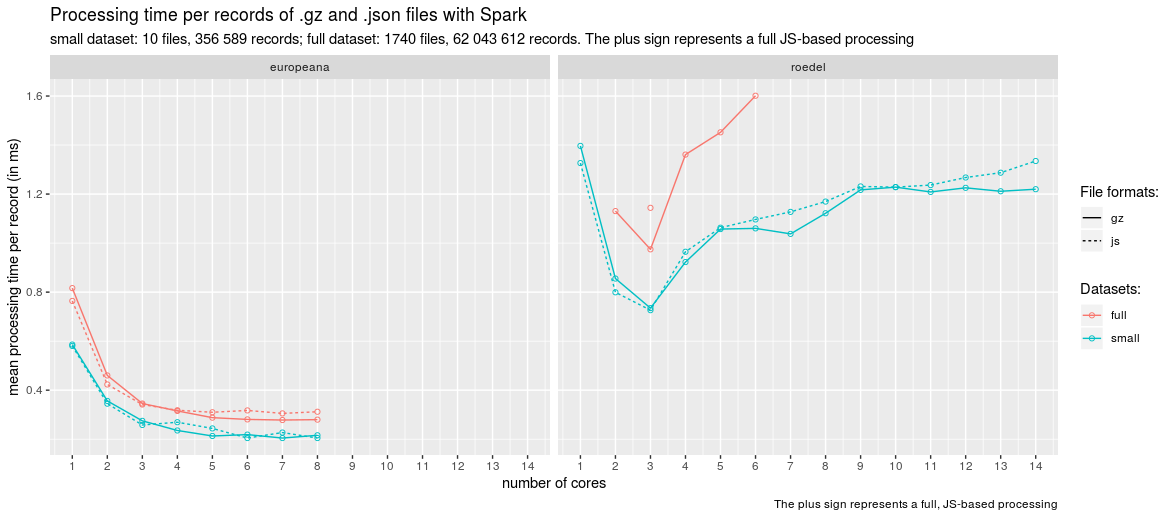
\includegraphics[width=\textwidth]{images/chapter06/small-and-full-measurements-two-servers.png}
\caption{Processing time per records with different settings}
\label{small-and-full-measurements-two-servers}
\end{figure}

1) The per record processing times for the small set is faster. It is not surprising given, that processing time depends on the complexity of the record structure which correlates with the size of the record. It is more important that the shape of the small set and the full set are close to each other, which means that running a small set for this kind of application might predict the running of the full set. An important factor is that the processing function (`measure()') is stateless, the incorporating classes do not collect data (unless in exceptional cases), so the measurement does not depend on previous records. Not all Spark client code works this way, so the statement about the prediction holds only for stateless ones.

2) Gzip compressed files are usually slightly faster than uncompressed. Processing compressed file has two side effects. First, uncompressed files are partitioned, and -- as we saw above -- each partition is paired with a distinct tasks, with its own overhead. Second, decompression also has its own overhead. The evident advantage of using compressed files is sparing of disk space. Note: since on `roedel' machine the full process took more than a day, and we did not had enough machine time, we just run the predictably fastest setting on uncompressed files.

3) The shape of lines on the two machines are significantly different. On `euroepana' the performance is continuously increasing up to 7 cores, but after a given number of cores the improvement is not significant. To find the optimal settings for the number of cores is not easy here, because there is no clear winner. One can decide on two factors, the first one being that the examined speed might be already 'good enough', the second being that while using more cores slightly improves the performance of the current process, it takes resources away from other processes running on the same system, which is an impolite behaviour. On `roedel' the situation is radically different; it has a clear peak at 3 cores. The general reason is that the system throughput (the combination of CPU, memory and I/O operation speed and other factors) has a maximum. If we run more processes parallel some of them consume all the available resources while some others have to wait for moments. To detect the actual bottleneck is not easy, we will see some techniques for this task later.

\subsection{Memory allocation}

The next setting under test is the amount of allocated memory. The process were run on the small, compressed set with different cores and allocating 1, 2, 3, and 4 GB memory for both Spark driver (the central controller) and executors (the parts which execute client code). The spark settings are available in Listing \ref{code:spark-memory}.

\begin{lstlisting}[
  % one can adjust spacing here if required
  % aboveskip=2.5\baselineskip,
  % belowskip=-.8\baselineskip,
  caption={Spark's memory allocation options},
  label=code:spark-memory,
  language=Bash,
  float]
spark-submit --driver-memory <memory> --executor-memory <memory> ...
\end{lstlisting}

\begin{figure}
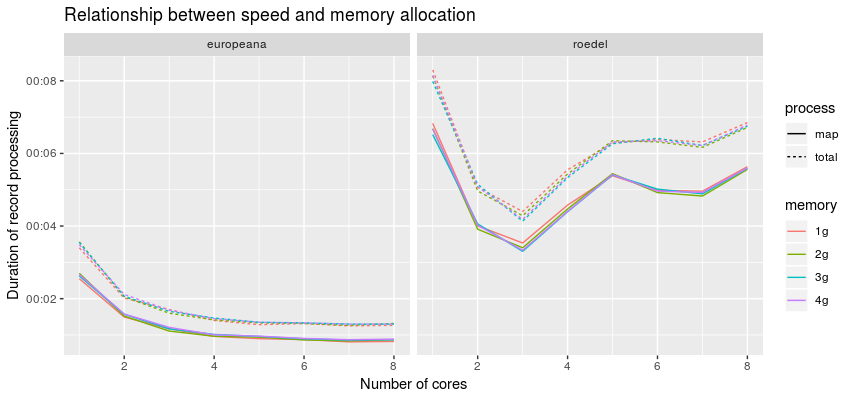
\includegraphics[width=\textwidth]{images/chapter06/memory-allocation-details.png}
\caption{Relationship between speed and memory allocation.}
\label{memory-allocation-details}
\end{figure}

Fig. \ref{memory-allocation-details} shows the result of different memory allocations. Succinctly, these settings do not have any clear effect. It is not a surprise, since the application is virtually stateless. If it would accumulate large (or lots of) variables in memory -- which happens in several Spark SQL or Spark ML based application -- we would see a different graph. The conclusion is that for this application it is not worth to allocate more memory than default (which is 1 GB for the current Spark version).

\subsection{HDFS or normal FS?}

Spark works well with Hadoop Distributed File System (HDFS)\footnote{\url{http://hadoop.apache.org/docs/current/hadoop-project-dist/hadoop-hdfs/HdfsDesign.html}}, but does it perform better in a standalone setup, where HDFS runs on a single machine, and is not distributed over nodes? The Spark settings is available in Listing \ref{code:hdfs}. The result is shown in Fig. \ref{hdfs-vs-fs}.

\begin{lstlisting}[
  % one can adjust spacing here if required
  % aboveskip=2.5\baselineskip,
  % belowskip=-.8\baselineskip,
  caption={Reading from HDFS},
  label=code:hdfs,
  language=Bash,
  float]
spark-submit --inputFileName hdfs://localhost:9000/europeana/*.gz ...
\end{lstlisting}


\begin{figure}
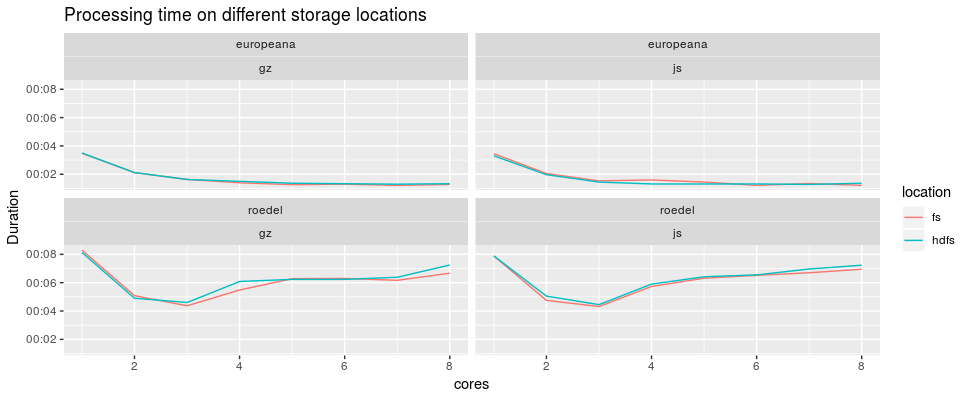
\includegraphics[width=\textwidth]{images/chapter06/hdfs-vs-fs.png}
\caption{Processing time on different storage locations}
\label{hdfs-vs-fs}
\end{figure}

In most cases the results are slightly better for OS file system, but not always, and usually the difference is small. The question whether it is worth to use HDFS or not depends on the speed gain and the cost of the setup of HDFS. In these systems the advantage does not hold, so it is not worth to store files in HDFS.

\section{Event log and history server -- to measure performance}

It was mentioned earlier that Spark launches a monitoring web service (unless it is disabled), which provides useful information about the running process. Although he application is shut down when the process ends, fortunately Spark provides a tool to keep history information persisted. It requires to set a directory into which the application stores the events alongside with their metrics. The history server is similar to the monitoring server, however it process data from the saved event log, and not from the live process. Since the event log is a simple text file containing JSON formatted lines, it is possible to move it and display the content on a different machine.\footnote{The event log file name consists of the master name and the timestamp of the start (such as `local-1550822115584'). This name is also used as an identifier inside the file. If you would like to use it in another machine, rename the file and change its identifier in its content (e.g. in this experiment we used names such as `europeana-c4').} It is very important to note that the web interface does not show all the information from the event log. History server provides an API, so the data could be programmatically read from it.

\begin{lstlisting}[
  % one can adjust spacing here if required
  % aboveskip=2.5\baselineskip,
  % belowskip=-.8\baselineskip,
  caption={Spark history server setting and launch},
  label=code:history-server,
  language=Bash,
  float]
> cd $SPARK_HOME
> more conf/spark-defaults.conf
...
spark.eventLog.enabled         true
spark.eventLog.dir             file:/path/to/spark-event-log
spark.history.fs.logDirectory  file:/path/to/spark-event-log
> sbin/start-history-server.sh
\end{lstlisting}

\begin{figure}
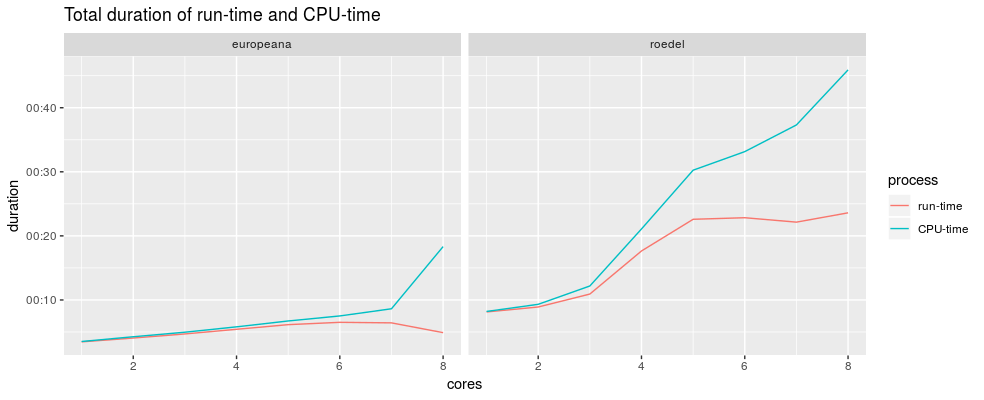
\includegraphics[width=\textwidth]{images/chapter06/runtime-vs-cputime-absolute.png}
\caption{Processing time on different storage locations}
\label{runtime-vs-cputime-absolute}
\end{figure}

The most important information for our experiment are `executorRunTime' and `executorCpuTime' variables. According to Spark API documentation \cite{spark-taskmetrics} `executorRunTime' is the "time the executor spends actually running the task (including fetching shuffle data)", while `executorCpuTime' is the "CPU Time the executor spends actually running the task (including fetching shuffle data) in nanoseconds". Since our process does not have shuffle steps, we can suppose that most of the time happens inside the map() function. According to \cite{canali2017} the difference between run-time and CPU-time is the time the CPU waits for the memory. Fig. \ref{runtime-vs-cputime-absolute} reveals that this time is getting larger and larger in both machines as we increase the number of cores. It is natural, because more and more process should compete for the resources. The two machines behave differently regarding to the increasing of this difference between times.

\begin{figure}
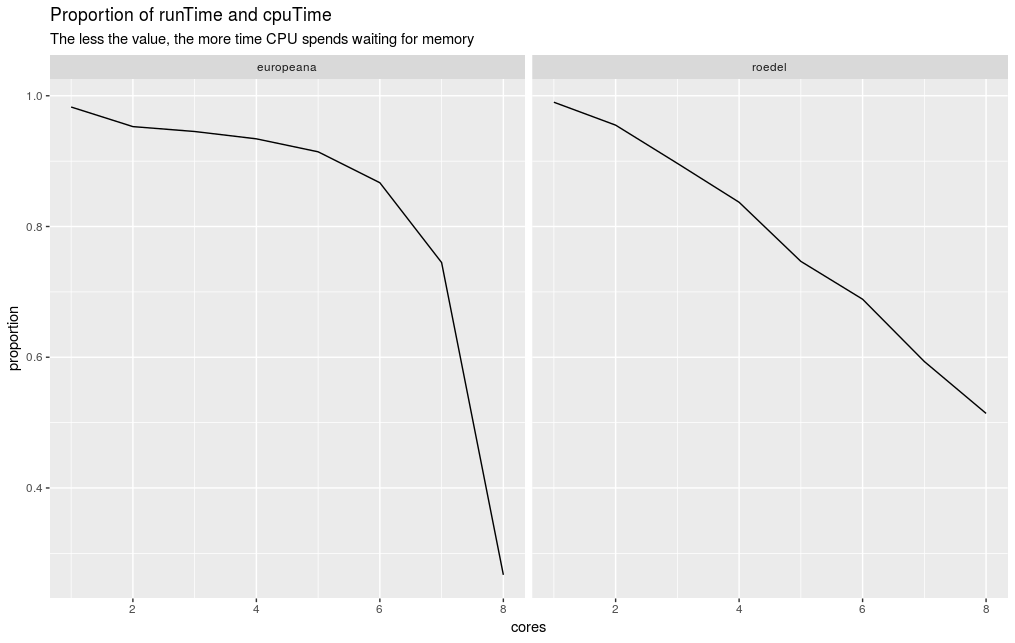
\includegraphics[width=\textwidth]{images/chapter06/runtime-vs-cputime.png}
\caption{Proportion of run-time and CPU-time. The larger the distance, the more time CPU is waiting.}
\label{runtime-vs-cputime}
\end{figure}

If we display it differently, highlighting the relative numbers i.e. the proportion of run-time and CPU-time in Fig. \ref{runtime-vs-cputime}, we see an interesting pattern. While in `europeana' the degradation is moderated up until 6 cores and from then progressive, on `roedel' it is linear. It means that the CPU is waiting a lot even when it performs well under small number of cores.

\begin{figure}
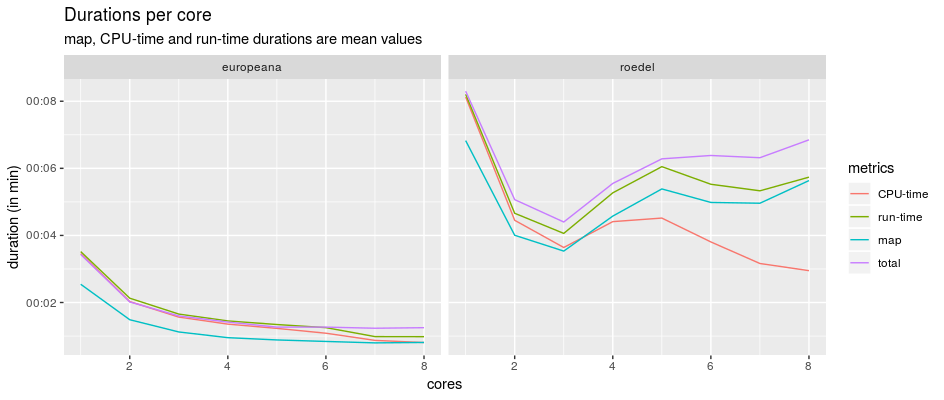
\includegraphics[width=\textwidth]{images/chapter06/all-durations.png}
\caption{Duration of different components per CPU.}
\label{all-durations}
\end{figure}

In the last figure (Fig. \ref{all-durations}) along with run-time and CPU-time the time of map method and the total time is also displayed. It reveals the reason of the performance peak: the best performance happens before the time of map exceeds the CPU-time. It is not clear exactly what other processes involved in the task, but it is clear, that CPU does other things as well, because up to that crossing CPU-time is larger then map-time. But when map-time gets bigger than CPU-time, it is clear that map (and the other confounded processes) has to wait for free memory. This crossing happened on `europeana' between 7 and 8 cores, while on `roedel' between 3 and 4 cores. It is also interesting that at 8 cores on `roedel' the map-time is almost reach run-time, and almost half of it is spent for waiting.

One last note about the hidden processes. As mentioned earlier Spark optimizes its code, and it is not the high level API which finally runs in the JVM. Another important feature of this API is that the methods are classified either as transformations or as actions. In Spark nothing happens until an action triggers the launch of the processing workflow, in which the transformations happen in a pipeline manner. It has two important consequences. First, the duration of some methods can not be measured in the client code, because it only assembles the building blocks, but not runs it. Second, there is no clear mapping between client code, and what a Java profiler shows, not just because of the optimization process, but also because of intensive usage of language constructions such as lambda functions. For example textFile() method which reads the file is not shown up in the Java stack trace.

\section{Conclusion}

The most important lessons learned in this experiment is that allocating more resources does not necessary imply better performance, and what we really need in an environment with limited and shared resources is a `good enough' state which politely let other processes run. To find the optimal settings it is suggested to pick up a smaller sample, which is similar to the full dataset in important characteristics, and measure speed with different settings. The settings worth to check are number of cores, memory allocation, compression of the source files, and different file systems (if they are available). As a source of ground truth one can use Spark log (which contains some performance indicator), Spark event log (disabled by default), or measuring points in your application (via Spark accumulators \cite{spark-accumulators}).

% \bibliographystyle{acm}
% \bibliography{bibliography-for-papers}

\chapter{Conclusion}

\section{Results}

It is worth to retrospect shortly to my research plan~\cite{kiraly2015a}, which was written before starting the actual research. I wanted to implement as much metadata metrics defined by~\cite{bruce-hillmann2004, ochoa-duval2009} as possible (some of these metrics would have required access to the full text of books or articles, which were not given in Europeana -- so it was not guaranteed that each metrics are implementable in the current context). The main research question was if it is possible to create an implementation of the metrics which is scalable (works both with large and small amount of metadata records) and flexible as well (adaptable to different metadata schemas).

During the research I had three tracks of activities

\begin{enumerate}
  \setlength{\parskip}{0pt}
  \setlength{\itemsep}{0pt plus 1pt}
\item Studying the metadata quality domain
\item Engineering the tool
\item Communicating about metadata quality and dissemination of the results
\end{enumerate}

In the first track I studied the metadata quality literature (including a portion of data and information quality literature). Since this domain is not a purely theoretical field, looking for current practice -- as far as it was possible -- I participated in or at least followed the activities of metadata quality projects and metadata quality related activities of digital libraries (among others Europeana, Deutsche Digitale Bibliothek, Digital Public Library of America). My interest was rather practical, and less theoretical. My special point of view was the question how the results of these papers could be turned into an Open Source software which could be used in different contexts, however during the process -- together with members of Europeana Data Quality Committee -- we also introduced a new metric we haven't found in the literature, which measures the multilingual aspects of metadata.

The main purpose of the engineering track was to create a general metadata quality measuring framework. It became a set of modules, such as a core Java API, an Europeana specific Java API, clients for them such as a REST API, a Spark interface, a web user interface, then a MARC 21 tool, a Wikidata-centric tool etc. each adding a specific purpose layer to the lower levels. The tool -- tested through different experiments -- proved to be both flexible (adaptable to different metadata schemas) and scalable.

The software packages created as part of the dissertation are:

\begin{itemize}
  \setlength{\parskip}{0pt}
  \setlength{\itemsep}{0pt plus 1pt}
\item Harvester client for Europeana's OAI-PMH server (\url{https://github.com/pkiraly/europeana-oai-pmh-client}). It turned out, that Europeana's OAI-PMH implementation is not robust enough to let clients to harvest the whole dataset. Later I was given access to a MongoDB server, and in most of the time I used this directly instead of using the OAI-PMH protocol.\footnote{Later the issues I found were reportedly fixed, however I haven't tested the service again.}
\item General Metadata QA API. Source code: \url{https://github.com/pkiraly/metadata-qa-api},
Maven\footnote{Maven is a Java building tool and a network of distributed Java library repositories. As a Java or Scala developer you can reuse others' libraries. These libraries has versions. The Maven repositories contain signed binary files and their metadata, which can be used in different Java projects independent from the building tool.} artifact (binary Java library): \url{http://mvnrepository.com/artifact/de.gwdg.metadataqa/metadata-qa-api}
\item The Europeana-specific Europeana QA Java API:
Source code: \url{https://github.com/pkiraly/europeana-qa-api},
Maven artifact: \url{http://mvnrepository.com/artifact/de.gwdg.metadataqa/europeana-qa-api}
\item Apache Spark interface of Europeana QA Java API: \url{https://github.com/pkiraly/europeana-qa-spark}
\item Analysis with R: \url{https://github.com/pkiraly/europeana-qa-r}. By the end of 2018 it became clear that the limitations of R as a language (mainly that it could process as much data as the size of the available memory) blocks the targetted monthly cycle of data analysis, so the whole analysis was rewritten in Scala with Spark API, which became part of the europeana-qa-spark codebase, and this R based code base will not have been updated in the future.
\item Web interface: \url{https://github.com/pkiraly/europeana-qa-web}
\item REST and command line interface: \url{https://github.com/pkiraly/europeana-qa-client}
\item Apache Solr connector: \url{https://github.com/pkiraly/europeana-qa-solr}
\item Cassandra connector: \url{https://github.com/pkiraly/europeana-qa-cassandra}
\item Metadata assessment for MARC records. Source code: \url{https://github.com/pkiraly/metadata-qa-marc}, Maven artifacts: \url{https://mvnrepository.com/artifact/de.gwdg.metadataqa/metadata-qa-marc} 
\item Web interface for displaying the result of the quality assessment of MARC records \url{https://github.com/pkiraly/metadata-qa-marc-web}
\item Quality assessment for the bibliographic records of Wikidata \url{https://github.com/pkiraly/metadata-qa-wikidata}
\item Supplementary materials for paper submitted to EURO-PAR conference \url{https://github.com/pkiraly/euro-par}
\end{itemize}

The third aspect of the research was the communication and  dissemination of the results which activity accumulated in the current dissertation. The list of presentations and papers published in the context of this presentation is available in Appendix C.

As we saw, metadata quality has multiple dimensions. For each data source we should select those which fit to them both theoretically and practically. The measures have their ``computational footprints'': the calculation require a given amounts of human and IT resources (and they are not always foreseeable) we should take it into account both in research and non-research projects. Another important aspect is the human condition: the metrics should not be something which is meaningful only from statistical viewpoint, they should be meaningful for the maintainer of data as well. The metrics should help a decision making process about the modification of the data. During the research it was the hardest point: to find the intersection of the interests with metadata experts. It repeatedly happened that what I provided as a result was not useful from the cataloguers' perspective, so I had to improve it based on the feedbacks. It was a pleasant situation, that during the research I worked together with an expert group, the Europeana Data Quality Committee, whose members provided me constant feedback (and requests too, naturally). This collaboration started in 2016, but the work hasn't yet finished, since we haven't reached a clear consensus on what information are useful.

I plan to continue this kind of research in the future, however a similar collaboration with institutions or experts is a strong necessity for any further research.

\section{Future work}

\subsection{Research data}

CoreTrustSeal is a certification for research data repositories, based on the DSA-WDS Core Trustworthy Data Repositories Requirements\footnote{see Core Trustworthy Data Repositories Extended Guidance v1.1 (June, 2018) \url{https://www.coretrustseal.org/wp-content/uploads/2017/01/20180629-CTS-Extended-Guidance-v1.1.pdf}}. The certification is a successor of Data Seal of Approval. Its purpose is prove that the certified repositories are following best practices of research data management. Organizations should explain their activities in 15 areas, such as data access, licences, workflow, data integrity etc. There are two areas which are interesting from the aspect of metadata quality measurement: appraisal and data quality. The certificates contain the organization's answer and the certifying institution's notes, and they are publicly available\footnote{\url{https://www.coretrustseal.org/why-certification/certified-repositories/}}. At the time of writing there are 54 CoreTrustSeal certified repositories. The certifications are quite interesting documents, and together they provide a kind of cross section of the state of the art in the 15 areas of data repositories. It seems that their data and metadata quality activities concentrate on the following topics:

\begin{itemize}
  \setlength{\parskip}{0pt}
  \setlength{\itemsep}{0pt plus 1pt}
  \item setting the list of recommended and accepted file formats, and checking incoming files against it
  \item documentation efforts on different levels (general, domain specific, national) creating manuals and guides both for the users and the maintainers of the repository
  \item data curation by experts -- most of these repositories are not self-service, the deposited materials are carefully checked by human experts. They check both the archival aspects (formats, metadata) and domain aspects (content relevancy)
  \item management of sensitive data (secure data management or excluding non anonymized data)
  \item setting mandatory, recommended and optional fields regarding to the metadata records
  \item online form validation -- for the metadata created via an online user interface
  \item some repositories apply XML validators when the metadata record is expected to be available in XML format
\end{itemize}

Among the traditional metadata quality dimensions only completeness is mentioned, and it is used as a synonym of the case when all of the mandatory fields are available in the metadata record (``Ensuring DDI fields are completed in the metadata ensures quality control of completeness.'' wrote the Australian Data Archive\footnote{\url{https://assessment.datasealofapproval.org/assessment_245/seal/html/}}). Only a small portion of repositories mentioned usage of controlled vocabulary, and in this preliminary research I found only one repository which named an independent tool used for automating the metadata quality check\footnote{FDAT, Tübingen uses docuteam packer see \url{https://wiki.docuteam.ch/doku.php?id=docuteam:packer}}. The Worldwide Protein Data Bank\footnote{\url{https://assessment.datasealofapproval.org/assessment_281/seal/html/}} mentioned that they created two kinds of representations of data quality assessment: one for specialists, and another for non-specialists. The later contains simple graphical depiction that ``highlights a small number of essential quality metrics''. Different repositories mentioned that they reuse good quality metadata records as examples in the documentation.

It is worth to quote the checklist of Digital Repository of Ireland\footnote{\url{https://repository.dri.ie/catalog/sj13pg68d}} in which they describe the recommended steps to conduct regular metadata quality assessments:

\begin{itemize}
  \setlength{\parskip}{0pt}
  \setlength{\itemsep}{0pt plus 1pt}
  \item Designate one or a small team of information professionals to take responsibility for the audit.
  \item Decide to what extent any mistakes found during the audit will be fixed within the live database.
  \item On a quarterly or biannual basis, upload a sample set of records to the software application OpenRefine.
  \item Use the Faceting and Cluster tools in OpenRefine to identify and record errors, such as misspellings, inconsistent use of capitalisation or blank cells.
  \item Compile the documentation so that any changes in quality can be noted over a period of time. This will be particularly useful if the organisation has recently started using new cataloguing methods.
\end{itemize}

The most widely used general metadata schemas are the elements of Data Documentation Initiative (DDI)\footnote{\url{http://www.ddialliance.org/}} framework,\footnote{DDI Lifecycle (\url{http://www.ddialliance.org/Specification/DDI-Lifecycle/3.2/XMLSchema/FieldLevelDocumentation/}) and DDI Codebook (\url{http://www.ddialliance.org/Specification/DDI-Codebook/2.5/XMLSchema/field_level_documentation.html})} and The Dublin Core Metadata Initiative's DCMI Metadata Terms\footnote{\url{http://www.dublincore.org/specifications/dublin-core/dcmi-terms/}}. Regarding to domain specific metadata schemas CLARIN's Component Metadata\footnote{\url{https://www.clarin.eu/content/component-metadata}} could be viewed as a domain specific standard in lingistic data repositories.

An important conclusion from this preliminary survey is that there is a kind of ``market gap'' both in research and tool development in the domain of research data management. The elements of data quality mentioned in the certificates (completeness, format consistency, content relevancy, checking facets for errors etc.) are not different than those elements one can find in other metadata domains. There are elements which exist, but apparently did not get so far the popularity they deserve, e.g. the ``frictionaless data'' data description metadata format~\cite{fowler2018} or FAIRmetrics~\cite{fairmetrics} I discussed in Chapter 1. Not to mention general elements of the metadata quality research (dimensions, metrics and tools), which could be introduced into this domain, for the satisfaction of both parties.

\subsection{Citation data}

Citation data, or bibliographic data of scholarly articles is a neuralgic point for the libraries. In the ``Western World'' and for large languages, the publishers are those players which traditionally built databases for the scholarly articles (such as Web of Knowledge, Scopus) instead of libraries. By and large there has been exceptions even in Western European countries. In case of smaller languages and for poorer countries the large publishers does not see the market value to publish scientific journals in vernacular languages therefore those journals are not covered in their databases. In the last two decades several different projects have been launched to make these metadata out of ``paywalls''. The largest of these project is the DOI database, but the larger part of DOI metadata is also not freely available, however the Initiative for Open Citations\footnote{\url{https://i4oc.org/}} works on making the citation data open. Recently WikiCite\footnote{\url{http://wikicite.org/}} is the largest freely available citation database based on the bibliographic data imported into Wikidata\footnote{\url{https://www.wikidata.org/wiki/Wikidata:Main_Page}}. It provides query interface and database dumps\footnote{\url{http://wikicite.org/access.html}}. Together with Jakob Voß, a volunteer of WikiCite and Wikidata we started a research project\footnote{Its code is en extension of the same codebase I wrote for the Europeana analysis. It is available at \url{https://github.com/pkiraly/metadata-qa-wikidata/wiki}.} to analyze the data. This research is in a preliminary stage. Now I highlight only one feature of the citation data namely \emph{page numbers}, which seems to be simple, but reveals some complex problems. One can expect that page numbers are arabic or roman numbers separated by dashes and commas (sometimes with some text before or after the numbers). I found however several hundred patterns, which do not fit this expectation. Here I show three issues with ``strange'' page numbers.

A note before the examples. Wikidata uses a language neutral notation for describing its semantic structure, the entities are denoted by `Q' and a number, while properties are denoted by `P' and a number. For example: P304 is the property of the page numbers. Its human readable label in English is ``page(s)''\footnote{\url{https://www.wikidata.org/wiki/Property:P304}}.

\subsubsection{1. Using article identifier as page number}

Example \#1. Q40154916\footnote{\url{https://www.wikidata.org/wiki/Q40154916}}: P304 = ``e0179574''

This article was published in PLoS ONE\footnote{\url{https://journals.plos.org/plosone/article?id=10.1371/journal.pone.0179574}}. The publisher provides citation text, and metadata in RIS and BibTeX format. The citation contains `e0179574', however it does not explain what exactly it means (as it neither explains any other elements):

Citation on the journal's page:

Vincent WJB, Harvie EA, Sauer J-D, Huttenlocher A (2017) \emph{Neutrophil derived LTB4 induces macrophage aggregation in response to encapsulated Streptococcus iniae infection.} PLoS ONE 12(6): e0179574. \url{https://doi.org/10.1371/journal.pone.0179574}

In the PDF version of the paper\footnote{\url{https://journals.plos.org/plosone/article/file?id=10.1371/journal.pone.0179574&type=printable}} there are page numbers. It also does not explain what `e0179574' means. 

Metadata in RIS\footnote{https://journals.plos.org/plosone/article/citation/ris?id=10.1371/journal.pone.0179574} (only the relevant part):
\begin{lstlisting}
SP  - e0179574
EP  - 
\end{lstlisting}

SP stands for starting page, EP stands for ending page. It is evident here, that `e0179574' is not a starting page.

The BibTeX version\footnote{\url{https://journals.plos.org/plosone/article/citation/bibtex?id=10.1371/journal.pone.0179574}} contains page number, however does not contain the article identifier at all:
\begin{lstlisting}
@article{10.1371/journal.pone.0179574,
  year = {2017},
  month = {06},
  volume = {12},
  pages = {1-16},
  ...
}
\end{lstlisting}

The DOI database follows the content of RIS metadata file instead of BibTeX\footnote{I used the Crossref API with the following command to retrieve a DOI metadata\\
\texttt{curl -H "Accept: application/rdf+xml" http://data.crossref.org/[DOI]}, such as http://data.crossref.org/10.1371/journal.pone.0179574}:

\begin{lstlisting}
<rdf:RDF xmlns:rdf="http://www.w3.org/1999/02/22-rdf-syntax-ns#"
    xmlns:j.1="http://prismstandard.org/namespaces/basic/2.1/"
    xmlns:j.2="http://purl.org/ontology/bibo/" ...>
  <rdf:Description rdf:about=".../10.1371/journal.pone.0179574">
    <j.2:pageStart>e0179574</j.2:pageStart>
    <j.1:startingPage>e0179574</j.1:startingPage>
    ...
  </rdf:Description>
</rdf:RDF>
\end{lstlisting}

Example \#2. Q21820630\footnote{\url{https://www.wikidata.org/wiki/Q21820630}}: P304 = ``c181''

This paper was published in the British Medical Journal\footnote{\url{https://www.bmj.com/content/340/bmj.c181}}. It does not have a PDF version, the only available online version is HTML.

Hrynaszkiewicz Iain, Norton Melissa L, Vickers Andrew J, Altman Douglas G. \emph{Preparing raw clinical data for publication: guidance for journal editors, authors, and peer reviewers} BMJ 2010; 340 :c181 \url{https://www.bmj.com/content/340/bmj.c181} (DOI: 10.1136/bmj.c181)

The RIS metadata\footnote{\url{https://www.bmj.com/highwire/citation/194003/ris}} contains bad page number, uses the article identifier:

\begin{lstlisting}
SP  - c181
\end{lstlisting}

In BibTex metadata\footnote{\url{https://www.bmj.com/highwire/citation/194003/bibtext}} there is no page number, but an `elocation-id` field is available:
\begin{lstlisting}
@article{Hrynaszkiewiczc181,
  elocation-id = {c181},
  ...
}
\end{lstlisting}

The DOI database follows again the RIS metadata file instead of BibTeX\footnote{\url{http://data.crossref.org/10.1136/bmj.c181}}, however it repeats the same string in ending page fields:

\begin{lstlisting}
  <j.1:startingPage>c181</j.1:startingPage>
  <j.2:pageStart>c181</j.2:pageStart>
  <j.1:endingPage>c181</j.1:endingPage>
  <j.2:pageEnd>c181</j.2:pageEnd>
\end{lstlisting}

A possible conclusion would be that if there is a BibTeX source available, and it doesn't have page number element, but elocation-id, it is a better source than the RIS version. 

JATS (Journal Archiving and Interchange Tag Library)\footnote{NISO JATS Version 1.1 (ANSI/NISO Z39.96-2015) \url{https://jats.nlm.nih.gov/archiving/tag-library/1.1/}} defines the \texttt{<elocation-id>} element as ``replaces the start and end page elements just described for electronic-only publications;''\footnote{\url{https://jats.nlm.nih.gov/archiving/tag-library/1.1/element/elocation-id.html}}.

In this journal (British Medical Journal) some article has a PDF version, (e.g. \url{https://doi.org/10.1136/bmj.d1584}, \url{https://doi.org/10.1136/bmj.e1454}, \url{https://doi.org/10.1136/bmj.a494}) where there are clearly page numbers. The journal provided RIS and BibTeX metadata do not contain page numbers in those cases.

\subsubsection{2. Wikidata contains extra info, which is not available elsewhere}

Q39877401\footnote{\url{https://www.wikidata.org/wiki/Q39877401}}: P304 = "108-17; quiz 118-9"

The article has been published in \emph{Orthopaedic Nursing}\footnote{\url{https://journals.lww.com/orthopaedicnursing/pages/articleviewer.aspx?year=2016&issue=03000&article=00010&type=abstract}}

Schroeder, Diana L.; Hoffman, Leslie A.; Fioravanti, Marie; Medley, Deborah Poskus; Zullo, Thomas G.; Tuite, Patricia K. \emph{Enhancing Nurses' Pain Assessment to Improve Patient Satisfaction} Orthopaedic Nursing: March/April 2016 - Volume 35 - Issue 2 - p 108–117. DOI: 10.1097/NOR.0000000000000226.

Page number in DOI\footnote{\url{http://data.crossref.org/10.1097/NOR.0000000000000226}} repeats the information provided at the journal:

\begin{lstlisting}
  <bibo:pageStart>108</bibo:pageStart>
  <prism:startingPage>108</prism:startingPage>

  <bibo:pageEnd>117</bibo:pageEnd>
  <prism:endingPage>117</prism:endingPage>
\end{lstlisting}

In the publisher's citation the page number contains the first part of the page number string of the Wikidata value, but not the ``; quiz 118-9'' part. In the table of contents there is another article\footnote{\url{https://journals.lww.com/orthopaedicnursing/Citation/2016/03000/Enhancing_Nurses__Pain_Assessment_to_Improve.11.aspx#print-article-link}, DOI: {10.1097/NOR.0000000000000236}} at page 118-119 of the same issue. It's title is the same, but it does not have authors recorded. It is categorised under ``CE Tests'' (where CE means continuing education). The two articles don't link directly to each other. They are different, and have different DOIs. The DOI database neither contains any link between them.

Wikidata should keep them separated, however it would require rather long time to investigate cases like this.

\subsubsection{3. Wikidata uses page number field to add comment}

Q28710224\footnote{\url{https://www.wikidata.org/wiki/Q28710224}}: P304 = "E3523; author reply E3524–5"

Alain Pierret, Valéry Zeitoun, Hubert Forestier: \emph{Irreconcilable differences between stratigraphy and direct dating cast doubts upon the status of Tam Pa Ling fossil.} Proceedings of the National Academy of Sciences Dec 2012, 109 (51) E3523; DOI: \url{http://doi.org/10.1073/PNAS.1216774109}, URL in journal: \url{https://www.pnas.org/content/109/51/E3523}, URL in Wikidata: \url{https://www.wikidata.org/wiki/Q28710224}.

E3524–5 is not part of the article. It is a related article, which is also available in Wikidata (as Q28710226\footnote{\url{https://www.wikidata.org/wiki/Q28710226}}):

Fabrice Demeter, Laura L. Shackelford, Kira E. Westaway, Philippe Duringer, Thongsa Sayavongkhamdy, and Anne-Marie Bacon: \emph{Reply to Pierret et al.: Stratigraphic and dating consistency reinforces the status of Tam Pa Ling fossil} PNAS December 18, 2012 109 (51) E3524-E3525; \url{https://doi.org/10.1073/pnas.1217629109}, URL in journal: \url{https://www.pnas.org/content/109/51/E3524}.

These two articles are not interlinked with distinct properties. One could suppose, that the occurrence `author reply' in other Wikidata records' page number could reveal similar hidden links.

\subsection{Fixing issues -- is that possible?}

The Swedish National Heritage Board just launched a project called \emph{Wikimedia Commons Data Roundtripping}\footnote{\url{https://outreach.wikimedia.org/wiki/GLAM/Newsletter/February_2019/Contents/Special_story}}. \emph{Roundtripping} is the name of the workflow in which a cultural heritage institution publish their data in Wikimedia Commons, the users enrich these openly available media (such as adding translations of descriptive texts into other languages, identifying people, names and aliases, locations and subject matter or linking to authority data and using it to retrieve third party contributions from other memory organisations), then institutions ingest these data and update their original database.

Wikidata doesn't seem to be the platform where the data are generated, but rather it is a place where data created elsewhere are imported to and maybe enriched. Additionally, the bibliographical data in general seems to have their own data flow: from different sources they are duplicated into different targets, such as DOI database(s), commercial discovery interfaces (Scopus\footnote{\url{https://www.scopus.com/}}, Web of Science\footnote{\url{https://www.webofknowledge.com/}}, Google Scholar\footnote{\url{https://scholar.google.de/}}, Microsoft Academic\footnote{\url{https://academic.microsoft.com/}}, SpringerNature SciGraph\footnote{\url{https://scigraph.springernature.com/}}), institutional repositories, open data platforms (Wikidata, Wikipedia, DBPedia) etc. It is clear, that it would be impossible to fix the data in each platform, and probably the best place to fix them in their origin.\footnote{Ruben Verborgh, in his keynote speech at ELAG 2018 conference (``The delicate dance of decentralization and aggregation'' \url{http://slides.verborgh.org/ELAG-2018/}) suggested a researcher centric scholarly communication where the origin of the citation data is the researchers' own home pages, and aggregation services like those mentioned above harvest data from there.} It seems that DOI database is a kind of central hub in this network.

Who are responsible for metadata published in DOI database?

According to Göttingen eResearch Alliance's DOI experts Timo Gnadt and Sven Bingert DOI data is created and updated by the data providers, i.e. the institutions who own the data (usually they are the institutions behind the landing page of the metadata records), thus in our case they are the publishers of the journals.

In one case I wrote a report to Springer Nature regarding to the page numbers for Wilkinson et al, \emph{The FAIR Guiding Principles for scientific data management and stewardship},\footnote{Scientific Data volume 3, Article number: 160018 (2016) \url{https://www.nature.com/articles/sdata201618}} so far the discussion is about to clarify the problem, I do not have the publisher's opinion about the issue (and if they consider it as an issue).

This research could provide suggestions for Wikidata to fix the data in a format which could be used by bots to update the content. If such a fixing process is implemented, Wikidata's ingestion process should be aware of the updated information, to be sure that they are not overwritten by a next ingestion process. Also these corrections should be sent to the publishers.

\subsection{Participation in metadata quality activities}

In 2016 two important groups formed in the Cultural Heritage sector which started a deep investigation of data quality in particular segments: the Europeana Data Quality Committee\footnote{\url{http://pro.europeana.eu/page/data-quality-committee}} (DQC) and DLF Metadata Assessment Working Group\footnote{\url{https://dlfmetadataassessment.github.io/}} (MAWG). DQC examines the metadata issues specific to the Europeana collection, and involved in creating the measuring framework which is the main subject of this dissertation. The MAWG does not focus on a particular service and metadata schema, they collect relevant literature, use cases, and aims to form a set of recommendations on metadata assessment. In 2017 a Belgian project, ADOCHS\footnote{\url{http://adochs.be/}} (Auditing Digitalization Outputs in the Cultural Heritage Sector) started to improve the quality control process concerning the digitized heritage collections\footnote{The results of ADOCHS project could be found in the publications of Anne Chardonnens and Ettore Rizza -- see Appendix A.}. Similar activities of the Digital Public Library of America (DPLA) is described in~\cite{gueguen2019}.

I participated or followed the work of these groups. I am a member of DQC and contributed to the environmental scan task of MAWG. I presented my results in a MAWG virtual seminar, and I was a member of ADOCHS follow up committee.

As a last word I should note that I was successful in starting professional connections between a number of other actors, such as Deutsche Digitale Bibliothek, Bibliothèque National de France, DPLA, Metropolitan New York Library Council, University of North Texas libraries, etc., but rarely I was able to turn this initial sympathy into a fruitful collaboration. Although it is not a research purpose, but in the future I would like to improve those skills which are required for taking this additional step.

\section{Acknowledgement}

I would like to thank the help of Juliane Stiller, Zaveri Amrapali, Christina Harlow, Valentine Charles, Antoine Isaac. Thanks to the anonymous conference or journal reviewers who gave me important feedback.

Thanks to Philipp Wieder who encouraged me to conduct a PhD research, and to Gerhard Lauer, Ramin Yahyapour and Marco Büchler for supervising this research.

Thanks for GWDG for supporting my research in different ways. Thanks for Europeana and ETRAP research group for using their computers, for JetBrains s.r.o. providing me IntelliJ IDEA community licence. Special thanks for developers of Open Source software packages, and infrastructure services I used in the research.

\begin{otherlanguage}{magyar}
Köszönet Ildikónak, Zsófinak, Verának és Lucának szeretetükért és türelmükért. Családomnak és barátaimnak az eddigieket. -- „Lesznie kell!”
\end{otherlanguage}

\appendix
\chapter{Metadata assessment bibliography}

\chapterauthor{Péter Király, Sarah Potvin, Nikos Palavitsinis, Anna Neatrour, Ayla Stein, Sara R., Juliane Stiller, Kevin Clair, Pru Mitchell, Corey Harper, Christina Harlow, Laura Akerman, Laura J. Smart, David Maus, jenyoung, Kate Flynn, leonardaa, Cassandra Baker}

This bibliography is the result of a community effort. It was built on Zotero platform as Metadata Assessment Group Library\footnote{\url{https://www.zotero.org/groups/488224/metadata_assessment}}. The bibliography was initialized by Corey Harper in February 2016, and DFL Metadata Assessment working group used for recording items found during their environmental scan. Soon Europeana Data Quality Committee also started contributing to it. During my PhD research I intensively used it as well. According to the Zotero API\footnote{\url{https://api.zotero.org/groups/488224/items}. In order to retrieve every items, one should have an API key, and should use parameters `start' and `limit' (see Zotero API documentation at \url{https://www.zotero.org/support/dev/web_api/v3/basics}.} the creators of the bibliography entries are Péter Király (94 items), Sarah Potvin (32), Nikos Palavitsinis (18), Anna Neatrour, Ayla Stein, Sara R. (7), Juliane Stiller, Kevin Clair (4), Pru Mitchell, Corey Harper, Christina Harlow, Laura Akerman, Laura J. Smart (2), David Maus, jenyoung, Kate Flynn, leonardaa. Cassandra Baker contributed with improving of existing bibliography items.

\begin{center}
    *
\end{center}

\textsc{Acosta, M., Zaveri, A., Simperl, E., Kontokostas, D., Auer, S., and Lehmann, J.} 2013. Crowdsourcing Linked Data Quality Assessment. \emph{The Semantic Web – ISWC 2013}, Lecture Notes in Computer Science 8219. Heidelberg: Springer, 260–276. \url{https://doi.org/10.1007/978-3-642-41338-4_17}

\textsc{Albertoni, R., De Martino, M., and Podestà, P.} 2018. Quality measures for skos: ExactMatch linksets: an application to the thesaurus framework LusTRE. \emph{Data Technologies and Applications} \url{https://doi.org/10.1108/DTA-05-2017-0037}.

\textsc{Alemneh, D.G.} 2009. Metadata Quality Assessment: A Phased Approach to Ensuring Long-term Access to Digital Resources. \emph{Proceedings of the American Society for Information Science and Technology} \emph{46}, 1, 1–8 \url{https://doi.org/10.1002/meet.2009.1450460380}.

\textsc{Askham, N., Cook, D., Doyle, M., et al.} 2013. \emph{The Six Primary Dimensions For Data Quality Assessment. Defining Data Quality Dimensions}. DAMA UK. \url{https://www.whitepapers.em360tech.com/wp-content/files_mf/1407250286DAMAUKDQDimensionsWhitePaperR37.pdf}.

\textsc{Bade, D.} 2008. The Perfect Bibliographic Record: Platonic Ideal, Rhetorical Strategy or Nonsense? \emph{Cataloging \& Classification Quarterly} \emph{46}, 1, 109–133 \url{https://doi.org/10.1080/01639370802183081}.

\textsc{Barton, J., Currier, S., and Hey, J.M.N.} 2003. Building Quality Assurance into Metadata Creation: An Analysis based on the Learning Objects and e-Prints Communities of Practice. \emph{Papers and Project Reports for DC-2003 in Seattle, 28 September - 2 October 2003. Supporting Communities of Discourse and Practice}, 39–48 \url{http://dcpapers.dublincore.org/pubs/article/view/732}.

\textsc{Beall, J.} 2005. Metadata and Data Quality Problems in the Digital Library. \emph{Journal of Digital Information} \emph{6}, 3, 20.

\textsc{Bellini, E. and Nesi, P.} 2013. Metadata Quality Assessment Tool for Open Access Cultural Heritage Institutional Repositories. \emph{Information Technologies for Performing Arts, Media Access, and Entertainment}, Springer, 90–103. \url{https://doi.org/10.1007/978-3-642-40050-6_9}.

\textsc{Bellini, P., Bruno, I., Nesi, P., and Paolucci, M.} 2015. IPR Centered Institutional Service and Tools for Content and Metadata Management. \emph{International Journal of Software Engineering and Knowledge Engineering} \emph{25}, 08, 1237–1270. \url{https://doi.org/10.1142/S0218194015500242}.

\textsc{Bruce, T.R. and Hillmann, D.I.} 2004. The Continuum of Metadata Quality: Defining, Expressing, Exploiting. In: D. Hillman and E. Westbrooks, eds., \emph{Metadata in practice}. ALA Editions, Chicago, IL, 238–256.  \url{http://ecommons.cornell.edu/handle/1813/7895}.

\textsc{Bruce, T.R. and Hillmann, D.I.} 2013. Metadata Quality in a Linked Data Context. \url{https://blog.law.cornell.edu/voxpop/2013/01/24/metadata-quality-in-a-linked-data-context}.

\textsc{Cai, L. and Zhu, Y.} 2015. The Challenges of Data Quality and Data Quality Assessment in the Big Data Era. \emph{Data Science Journal} \emph{14}, 2 \url{https://doi.org/10.5334/dsj-2015-002}.

\textsc{Cechinel, C., da Silva Camargo, S., Sánchez-Alonso, S., and Sicilia, M.-Á.} 2012. On the Search for Intrinsic Quality Metrics of Learning Objects. \emph{Metadata and Semantics Research}, Springer, 49–60 \url{https://doi.org/10/gfphbr}.

\textsc{Cechinel, C., da Silva Camargo, S., Sicilia, M.-Á., and Sánchez-Alonso, S.} 2016. Mining Models for Automated Quality Assessment of Learning Objects. \emph{Journal of Universal Computer Science} \emph{22}, 1, 94–113. \url{https://doi.org/10.3217/jucs-022-01-0094}.

\textsc{Charbonneau, M.} 2005. Production benchmarks for catalogers in academic libraries: are we there yet? \emph{Library Resources and Technical Services} \emph{49}, 1, 40–48.

\textsc{Charles, V., Stiller, J., Király, P., Bailer, W., and Freire, N.} 2018. Data Quality Assessment in Europeana: Metrics for Multilinguality. \emph{Joint Proceedings of the 1st Workshop on Temporal Dynamics in Digital Libraries (TDDL 2017), the (Meta)-Data Quality Workshop (MDQual 2017) and the Workshop on Modeling Societal Future (Futurity 2017) (TDDL\_MDQual\_Futurity 2017) co-located with 21st International Conference on Theory and Practice of Digital Libraries (TPLD 2017), Grand Hotel Palace, Thessaloniki, Greece, 21 September 2017}, CEUR Workshop Proceedings. \url{http://ceur-ws.org/Vol-2038/paper6.pdf}.

\textsc{Chen, H.-H., Wu, J., and Giles, C.L.} 2018. Compiling Keyphrase Candidates for Scientific Literature Based on Wikipedia. \emph{Joint Proceedings of the 1st Workshop on Temporal Dynamics in Digital Libraries (TDDL 2017), the (Meta)-Data Quality Workshop (MDQual 2017) and the Workshop on Modeling Societal Future (Futurity 2017) (TDDL\_MDQual\_Futurity 2017) co-located with 21st International Conference on Theory and Practice of Digital Libraries (TPLD 2017), Grand Hotel Palace, Thessaloniki, Greece, 21 September 2017}, CEUR Workshop Proceedings. \url{http://ceur-ws.org/Vol-2038/paper6.pdf}.

\textsc{Chen, Y.-N., Wen, C.-Y., Chen, H.-P., Lin, Y.-H., and Sum, H.-C.} 2011. Metrics for metadata quality assurance and their implications for digital libraries. \emph{Digital Libraries: For Cultural Heritage, Knowledge Dissemination, and Future Creation (Proceedings of the 13th International Conference on Asia-Pacific Digital Libraries, 24–27 October 2011, Beijing, China.)}, Springer, 138–147. \url{http://ceur-ws.org/Vol-2038/paper4.pdf}.

\textsc{Clair, K.} 2016. Technical Debt as an Indicator of Library Metadata Quality. \emph{D-Lib Magazine} \emph{22}, 11/12. \url{https://doi.org/10.1007/978-3-642-24826-9_19}.

\textsc{Clements, K., Pawlowski, J., and Manouselis, N.} 2014. Why Open Educational Resources Repositories fail - Review of Quality Assurance Approaches. \emph{EDULEARN14 Proceedings. 6th International Conference on Education and New Learning Technologies Barcelona, Spain, 2014}, IATED, International Association of Technology, Education and Development, 929–939. \url{https://doi.org/10.1016/j.chb.2015.03.026}.

\textsc{Clements, K., Pawlowski, J., and Manouselis, N.} 2015. Open educational resources repositories literature review – Towards a comprehensive quality approaches framework. \emph{Computers in Human Behavior} \emph{51, Part B}, 1098–1106. \url{https://jyx.jyu.fi/dspace/handle/123456789/44031}.

\textsc{Conrad, S.} 2015. Using Google Tag Manager and Google Analytics to track DSpace metadata fields as custom dimensions. \emph{The Code4Lib Journal} 27. \url{http://journal.code4lib.org/articles/10311}.

\textsc{Debattista, J., Auer, S., and Lange, C.} 2016. Luzzu - A methodology and framework for linked data quality assessment. \emph{Journal of Data and Information Quality} \emph{8}, 1, 4:1-4:32. \url{https://doi.org/10.1145/2992786}.

\textsc{Debattista, J., Lange, C., and Auer, S.} 2014. Representing Dataset Quality Metadata using Multi-Dimensional Views. \emph{SEM ’14. Proceedings of the 10th International Conference on Semantic Systems}, ACM, 92–99. \url{https://doi.org/10.1145/2660517.2660525}.

\textsc{Decourselle, J., Duchateau, F., Aalberg, T., Takhirov, N., and Lumineau, N.} 2016a. Open datasets for evaluating the interpretation of bibliographic records. \emph{Proceedings of the 16th ACM/IEEE-CS on Joint Conference on Digital Libraries}, ACM, 253–254. \url{https://doi.org/10.1145/2910896.2925457}.

\textsc{Decourselle, J., Duchateau, F., Aalberg, T., Takhirov, N., and Lumineau, N.} 2016b. BIB-R: A Benchmark for the Interpretation of Bibliographic Records. \emph{Research and Advanced Technology for Digital Libraries}, Springer International Publishing, 163–174. \url{https://doi.org/10.1007/978-3-319-43997-6}.

\textsc{Degerstedt, S. and Philipson, J.} 2016. Lessons Learned from the First Year of E-Legal Deposit in Sweden: Ensuring Metadata Quality in an Ever-Changing Environment. \emph{Cataloging \& Classification Quarterly} \emph{54}, 7, 468–482. \url{https://doi.org/10.1080/01639374.2016.1197170}.

\textsc{Diakopoulos, N., Friedler, S., Arenas, M., et al.} 2016. Principles for Accountable Algorithms and a Social Impact Statement for Algorithms. \url{http://www.fatml.org/resources/principles-for-accountable-algorithms}.

\textsc{DLF Aquifer Metadata Working Group and Digital Library Federation}. 2009. \emph{Digital Library Federation / Aquifer Implementation Guidelines for Shareable MODS Records, version 1.1}. Digital Library Federation. \url{https://wiki.dlib.indiana.edu/display/DLFAquifer/DLF+Aquifer+Public+Metadata+Documents?preview=/28330/120160257/DLFMODS_ImplementationGuidelines.pdf}.

\textsc{DLF/NSDL Working Group on OAI PMH Best Practices}. 2007. \emph{Best Practices for OAI PMH DataProvider Implementations and Shareable Metadata}. Digital Library Federation, Washington, D.C. \url{https://old.diglib.org/pubs/dlf108.pdf}.

\textsc{Dodds, L.} Quality Indicators for Linked Data Datasets. \url{http://answers.semanticweb.com/questions/1072/quality-indicators-for-linked-data-datasets}.

\textsc{Doorn, P. and Tsoupra, E.} 2018. A Simple Approach to Assessing the FAIRness of Data in Trusted Digital Repositories. \emph{Joint Proceedings of the 1st Workshop on Temporal Dynamics in Digital Libraries (TDDL 2017), the (Meta)-Data Quality Workshop (MDQual 2017) and the Workshop on Modeling Societal Future (Futurity 2017) (TDDL\_MDQual\_Futurity 2017) co-located with 21st International Conference on Theory and Practice of Digital Libraries (TPLD 2017), Grand Hotel Palace, Thessaloniki, Greece, 21 September 2017}, CEUR Workshop Proceedings. \url{http://ceur-ws.org/Vol-2038/invited2.pdf}.

\textsc{DPLAFest Participants}. 2015. Metadata Quality Research. \url{https://docs.google.com/document/d/15pmA276_fxShkCEagoloJwCXH89PhrF3qWBgB8xSrag/edit\#}.

\textsc{Dublin Core Metadata Initiative}. 2014. DCMI Task Group RDF Application Profiles. \url{http://wiki.dublincore.org/index.php/RDF_Application_Profiles}.

\textsc{Durco, M. and Windhouwer, M.} 2014. The CMD Cloud. \emph{Proceedings of LREC 2014}, 687–690. \url{http://www.lrec-conf.org/proceedings/lrec2014/pdf/156_Paper.pdf}.

\textsc{Dushay, N. and Hillmann, D.I.} 2003. Analyzing Metadata for Effective Use and Re-Use. \emph{Proceedings, Dublin Core Metadata Conference, DC-2003}, Dublin Core Metadata Initiative. \url{http://dcpapers.dublincore.org/pubs/article/view/744}.

\textsc{Efron, M.} 2007. Metadata Use in OAI-Compliant Institutional Repositories. \emph{Journal of Digital Information} \emph{8}, 2. \url{http://people.ischool.illinois.edu/~mefron/papers/efron-metadatause.pdf}.

\textsc{Ellefi, M.B., Bellahsene, Z., Breslin, J., et al.} 2017. RDF Dataset Profiling - a Survey of Features, Methods, Vocabularies and Applications. \emph{Semantic Web} \emph{Preprint}, Preprint. \url{http://www.semantic-web-journal.net/content/rdf-dataset-profiling-survey-features-methods-vocabularies-and-applications}.

\textsc{Europeana Tech}. 2015. Evaluation and Enrichments Task Report Outcomes. \url{http://pro.europeana.eu/get-involved/europeana-tech/europeanatech-task-forces/evaluation-and-enrichments}.

\textsc{Färber, M., Bartscherer, F., Menne, C., and Rettinger, A.} 2017. Linked data quality of DBpedia, Freebase, OpenCyc, Wikidata, and YAGO. \emph{Semantic Web} \emph{Preprint}, Preprint, 1–53. \url{https://doi.org/10.3233/SW-170275}.

\textsc{Fischer, K.S.} 2005. Critical Views of LCSH, 1990–2001: The Third Bibliographic Essay. \emph{Cataloging \& Classification Quarterly} \emph{41}, 1, 63–109. \url{https://doi.org/10.1300/J104v41n01_05}.

\textsc{Foulonneau, M.} 2007. Information redundancy across metadata collections. \emph{Information Processing \& Management} \emph{43}, 3, 740–751. \url{http://dx.doi.org/10.1016/j.ipm.2006.06.004}.

\textsc{Foulonneau, M. and Cole, T.W.} 2005. Strategies for Reprocessing Aggregated Metadata. \emph{Research and Advanced Technology for Digital Libraries}, Springer Berlin Heidelberg, 290–301. \url{https://www.researchgate.net/profile/Muriel_Foulonneau/publication/221176072_Strategies_for_Reprocessing_Aggregated_Metadata/links/54173a450cf2f48c74a403d1.pdf}.

\textsc{Foulonneau, M. and Riley, J.} 2008. \emph{Metadata for Digital Resources: Implementation, Systems Design and Interoperability}. Chandos Publishing, Oxford.

\textsc{Fowler, D., Barratt, J., and Walsh, P.} 2018. Frictionless Data: Making Research Data Quality Visible. \emph{International Journal of Digital Curation} \emph{12}, 2, 274–285. \url{https://doi.org/10.2218/ijdc.v12i2.577}.

\textsc{Friesen, N.} 2004. \emph{International LOM Survey: Report (Draft)}. \url{http://arizona.openrepository.com/arizona/bitstream/10150/106473/1/LOM_Survey_Report2.doc}.

\textsc{Fürber, C. and Hepp, M.} 2011. Towards a Vocabulary for Data Quality Management in Semantic Web Architectures. \url{http://www.slideshare.net/cfuerber/towards-a-vocabulary-for-data-quality-management-in-semantic-web-architectures}.

\textsc{Gavrilis, D., Makri, D.-N., Papachristopoulos, L., et al.} 2015. Measuring Quality in Metadata Repositories. \emph{Proceedings from the 19th International Conference on Theory and Practice of Digital Libraries}, Springer, 56–67. \url{https://doi.org/10.1007/978-3-319-24592-8_5}.

\textsc{Gendered Expectations for Leadership in Libraries – In the Library with the Lead Pipe}. \url{http://www.inthelibrarywiththeleadpipe.org/2015/libleadgender/}.

\textsc{GO FAIR Metrics Group}. FAIR Metrics. \url{http://fairmetrics.org/}.

\textsc{Gonçalves, M.A., Moreira, B.L., Fox, E.A., and Watson, L.T.} 2007. “What is a good digital library?” – A quality model for digital libraries. \emph{Information Processing \& Management} \emph{43}, 5, 1416–1437. \url{https://doi.org/10.1016/j.ipm.2006.11.010}.

\textsc{Goovaerts, M. and Leinders, D.} 2012. Metadata quality evaluation of a repository based on a sample technique. \emph{Metadata and Semantics Research}, Springer, 181–189. \url{https://doi.org/10/gfphbs}.

\textsc{Greenberg, J., Spurgin, K., and Crystal, A.} 2005. \emph{Final Report for the AMeGA (Automatic Metadata Generation Applications) Project}. \url{http://www.loc.gov/catdir/bibcontrol/lc_amega_final_report.pdf}.

\textsc{Groskopf, C.} 2015. The Quartz guide to bad data. \emph{Quartz}. \url{https://qz.com/572338/the-quartz-guide-to-bad-data/}.

\textsc{Gueguen, G.} 2019. Metadata quality at scale: Metadata quality control at the Digital Public Library of America. \emph{Journal of Digital Media Management} \emph{7}, 2, 115–126.

\textsc{Guinchard, C.} 2006. Dublin Core use in libraries: a survey. \emph{OCLC Systems \& Services: International digital library perspectives} \emph{18}, 1, 40–50. \url{https://doi.org/10.1108/10650750210418190}.

\textsc{Guy, M., Powell, A., and Day, M.} 2004. Improving the Quality of Metadata in Eprint Archives. \emph{Ariadne} 38. \url{http://www.ariadne.ac.uk/issue38/guy/}.

\textsc{Harper, C.} 2016. Metadata Analytics, Visualization, and Optimization: Experiments in statistical analysis of the Digital Public Library of America (DPLA). \emph{The Code4Lib Journal} 33. \url{http://journal.code4lib.org/articles/11752}.

\textsc{Haslhofer, B. and Klas, W.} 2010. A survey of techniques for achieving metadata interoperability. \emph{ACM Computing Surveys} \emph{42}, 2, 1–37. \url{https://doi.org/10.1145/1667062.1667064}. \url{https://doi.org/10.1145/1667062.1667064}.

\textsc{Hillmann, D.I.} 2008. Metadata Quality: From Evaluation to Augmentation. \emph{Cataloging \& Classification Quarterly} \emph{46}, 1, 65–80. \url{https://doi.org/10.1080/01639370802183008}.

\textsc{Hillmann, D.I., Dushay, N., and Phipps, J.} 2004. Improving Metadata Quality: Augmentation and Recombination. \url{http://www.cs.cornell.edu/naomi/DC2004/MetadataAugmentation--DC2004.pdf}.

\textsc{Höffernig, M., Orgel, T., Russegger, S., and Bailer, W.} 2015. Assessing Quality in Automated Metadata Aggregation and Mapping Services. EEXCEES, 1–6. \url{http://eexcess.eu/wp-content/uploads/2013/03/JoanneumResearch_Assessing_Quality.pdf}.

\textsc{Höffernig, M., Orgel, T., Russegger, S., and Bailer, W.} 2013. Assessing Quality in Automated Metadata Aggregation and Mapping Services. \url{http://eexcess.eu/wp-content/uploads/2013/03/JoanneumResearch_Assessing_Quality.pdf}.

\textsc{van Hooland, S.} 2009. Metadata Quality in the Cultural Heritage Sector: Stakes, Problems and Solutions. \url{http://homepages.ulb.ac.be/~svhoolan/these.pdf}.

\textsc{Huang, Y. and Chiang, F.} 2018. Refining Duplicate Detection for Improved Data Quality. \emph{Joint Proceedings of the 1st Workshop on Temporal Dynamics in Digital Libraries (TDDL 2017), the (Meta)-Data Quality Workshop (MDQual 2017) and the Workshop on Modeling Societal Future (Futurity 2017) (TDDL\_MDQual\_Futurity 2017) co-located with 21st International Conference on Theory and Practice of Digital Libraries (TPLD 2017), Grand Hotel Palace, Thessaloniki, Greece, 21 September 2017}, CEUR Workshop Proceedings. \url{http://ceur-ws.org/Vol-2038/paper3.pdf}.

\textsc{Hughes, B.} 2004. Metadata Quality Evaluation: Experience from the Open Language Archives Community. \emph{Digital Libraries: International Collaboration and Cross-Fertilization}, Springer, 320–329. \url{https://doi.org/10.1007/978-3-540-30544-6_34}.

\textsc{Jackson, A., Han, M.-J., Groetsch, K., Mustafoff, M., and Cole, T.W.} 2008. Dublin Core Metadata Harvested Through OAI-PMH. \emph{Journal of Library Metadata} \emph{8}, 1, 5–21. \url{https://doi.org/10.1080/10911360802076682}.

\textsc{Jay, M., Simpson, B., and Smith, D.} 2009. CatQC and Shelf-Ready Material: Speeding Collections to Users While Preserving Data Quality. \emph{Information Technology and Libraries} \emph{28}, 1, 41–48. \url{https://doi.org/10.6017/ital.v28i1.3171}.

\textsc{Kaffee, L.-A., Piscopo, A., Vougiouklis, P., Simperl, E., Carr, L., and Pintscher, L.} 2017. A glimpse into babel: An analysis of multilinguality in wikidata. \emph{OpenSym ’17 Proceedings of the 13th International Symposium on Open Collaboration}, ACM, 14:1--14:5. \url{https://doi.org/10.1145/3125433.3125465}.

\textsc{Kaffee, L.-A. and Simperl, E.} 2018. The human face of the web of data: a cross-sectional study of labels. 66–77. \url{https://doi.org/10.1016/j.procs.2018.09.007}.

\textsc{Kapidakis, S.} 2012. Comparing metadata quality in the Europeana context. \emph{PETRA ’12 Proceedings of the 5th International Conference on PErvasive Technologies Related to Assistive Environments. Heraklion, Crete, Greece — June 06 - 08, 2012}, ACM, 25:1-25:8. \url{https://doi.org/10.1145/2413097.2413129}.

\textsc{Kapidakis, S.} 2015. Rating quality in metadata harvesting. \emph{PETRA ’15 Proceedings of the 8th ACM International Conference on PErvasive Technologies Related to Assistive Environments. Article No. 65. Corfu, Greece — July 01 - 03, 2015.}, ACM, 65:1-65:8. \url{https://doi.org/10.1145/2769493.2769512}.

\textsc{Kelly, B., Closier, A., and Hiom, D.} 2005. Gateway Standardization: A Quality Assurance Framework for Metadata. \emph{Library Trends} \emph{53}, 4, 637–650.

\textsc{Király, P.} 2015a. Metadata Quality Assurance Framework. \url{http://pkiraly.github.io/}.

\textsc{Király, P.} 2015b. A Metadata Quality Assurance Framework. Research plan. \url{http://pkiraly.github.io/metadata-quality-project-plan.pdf}.

\textsc{Király, P.} 2017. Towards an extensible measurement of metadata quality. \emph{DATeCH2017: Proceedings of the 2nd International Conference on Digital Access to Textual Cultural Heritage}, ACM, 111–115. \url{https://doi.org/10.1145/3078081.3078109}.

\textsc{Király, P. and Büchler, M.} 2018. Measuring completeness as metadata quality metric in Europeana. \emph{2018 IEEE International Conference on Big Data (Big Data)}, IEEE, 2711–2720. \url{https://doi.org/10.1109/BigData.2018.8622487}.

\textsc{Király, P., Stiller, J., Charles, V., Bailer, W., and Freire, N.} 2019. Evaluating Data Quality in Europeana: Metrics for Multilinguality. \emph{Metadata and Semantic Research}, Springer International Publishing, 199–211. \url{https://doi.org/10.1007/978-3-030-14401-2_19}.

\textsc{Kontokostas, D., Mader, C., Dirschl, C., et al.} 2016. Semantically Enhanced Quality Assurance in the JURION Business Use Case. \emph{The Semantic Web. Latest Advances and New Domains. ESWC 2016}, Springer, 661–676. \url{https://doi.org/10.1007/978-3-319-34129-3_40}.

\textsc{Kontokostas, D., Zaveri, A., Auer, S., and Lehmann, J.} 2013. TripleCheckMate: A Tool for Crowdsourcing the Quality Assessment of Linked Data. Springer, 265–272. \url{https://doi.org/10.1007/978-3-642-41360-5_22}.

\textsc{Koster, L.} 2014. Analysing library data flows for efficient innovation. \emph{Commonplace.net}. \url{http://commonplace.net/2014/11/library-data-flows/}.

\textsc{Lagoze, C., Krafft, D.B., Jesuroga, S., Cornwell, T., Cramer, E.J., and Shin, E.} 2005. An Information Network Overlay Architecture for the NSDL. \emph{JCDL ’05 Proceedings of the 5th ACM/IEEE-CS joint conference on Digital libraries}, ACM, 384–384. \url{https://doi.org/10.1145/1065385.1065487}.

\textsc{Lei, Y., Sabou, M., López, V., Zhu, J., Uren, V.S., and Motta, E.} 2006. An Infrastructure for Acquiring High Quality Semantic Metadata. \emph{The Semantic Web: Research and Applications}, Springer, 230–244. \url{https://doi.org/10.1007/11762256_19}.

\textsc{Lim, S. and Li Liew, C.} 2011. Metadata quality and interoperability of GLAM digital images. \emph{Aslib Proceedings} \emph{63}, 5, 484–498. \url{https://doi.org/10.1108/00012531111164978}.

\textsc{Lopatin, L.} Metadata Practices in Academic and Non-Academic Libraries for Digital Projects: A Survey. \emph{Cataloging \& Classification Quarterly} \emph{48}, 8, 716–742. \url{http://dx.doi.org/10.1080/01639374.2010.509029}.

\textsc{Loshin, D.} 2013. Building a Data Quality Scorecard for Operational Data Governance. \url{http://www.sas.com/content/dam/SAS/en_us/doc/whitepaper1/building-data-quality-scorecard-for-operational-data-governance-106025.pdf}.

\textsc{Lovins, D. and Hillmann, D.I.} 2017. Broken-World Vocabularies. \emph{D-Lib Magazine} \emph{23}, 3/4 (March/April). \url{https://doi.org/10.1045/march2017-lovins}.

\textsc{Ma, S., Lu, C., Lin, X., and Galloway, M.} 2009. Evaluating the metadata quality of the IPL. \emph{Proceedings of the American Society for Information Science and Technology} \emph{46}, 1, 1–17. \url{https://doi.org/10.1002/meet.2009.1450460249}.

\textsc{Mader, C., Haslhofer, B., and Isaac, A.} 2012. Finding Quality Issues in SKOS Vocabularies. \emph{Theory and Practice of Digital Libraries: Second International Conference, TPDL 2012, Paphos, Cyprus, September 23-27, 2012. Proceedings}, Springer, 222–233. \url{https://doi.org/10.1007/978-3-642-33290-6_25}.

\textsc{Madnick, S.E., Wang, R.Y., Lee, Y.W., and Zhu, H.} 2009. Overview and Framework for Data and Information Quality Research. \emph{ACM Journal of Data and Information Quality} \emph{1}, 1, 1–22. \url{https://doi.org/10.1145/1515693.1516680}.

\textsc{Margaritopoulos, M., Margaritopoulos, T., Mavridis, I., and Manitsaris, A.} 2012. Quantifying and Measuring Metadata Completeness. \emph{Journal of the American Society for Information Science and Technology} \emph{63}, 4, 724–737. \url{https://doi.org/10.1002/asi.21706}.

\textsc{Margaritopoulos, T., Margaritopoulos, M., Mavridis, I., and Manitsaris, A.} 2008. A Conceptual Framework for Metadata Quality Assessment. \url{http://dcpapers.dublincore.org/pubs/article/view/923}.

\textsc{Margaritopoulos, T., Margaritopoulos, M., Mavridis, I., and Manitsaris, A.} 2009. A Fine-Grained Metric System for the Completeness of Metadata. \emph{Conference Paper in Communications in Computer and Information Science}, Springer, 83–94. \url{https://doi.org/10.1007/978-3-642-04590-5_8}.

\textsc{Matienzo, M.A. and Rudersdorf, A.} 2014. The Digital Public Library of America Ingestion Ecosystem: Lessons Learned After One Year of Large-Scale Collaborative Metadata Aggregation. 12–23. \url{http://dcpapers.dublincore.org/pubs/article/view/3700}.

\textsc{Micic, N., Neagu, D., Campean, I.F., and Habib Zadeh, E.} 2017. Towards a Data Quality Framework for Heterogeneous Data. \url{https://bradscholars.brad.ac.uk/bitstream/handle/10454/12323/PID4808071.pdf?sequence=3\&isAllowed=y}.

\textsc{MODS Guidelines Levels of Adoption}. 2009. \emph{MODS Guidelines Levels of Adoption - American Social History Online}. \url{https://wiki.dlib.indiana.edu/display/DLFAquifer/MODS+Guidelines+Levels+of+Adoption}.

\textsc{Moen, W.E., Stewart, E.L., and McClure, C.R.} 1997. \emph{The Role of Content Analysis in Evaluating Metadata for the U.S. Government Information Locator Service (GILS): Results from an Exploratory Study Citations, Rights, Re-Use}. University of North Texas Libraries, Digital Library. \url{https://digital.library.unt.edu/ark:/67531/metadc36312/}.

\textsc{Najjar, J. and Duval, E.} 2006. Actual Use of Learning Objects and Metadata: An Empirical Analysis. \emph{TCDL Bulletin} \emph{2}, 2. \url{http://www.ieee-tcdl.org/Bulletin/v2n2/najjar/najjar.html}.

\textsc{Najjar, J., Ternier, S., and Duval, E.} 2003. The actual use of metadata in Ariadne: an empirical analysis. \emph{Proc. ARIADNE 3rd International Conference (2003)}, 6. \url{http://citeseerx.ist.psu.edu/viewdoc/download?doi=10.1.1.93.3666\&rep=rep1\&type=pdf}.

\textsc{Neto, C.B., Kontokostas, D., Hellmann, S., Müller, K., and Brümmer, M.} 2016. Assessing Quantity and Quality of Links Between Linked Data Datasets. \emph{Proceedings of the Workshop on Linked Data on the Web co-located with the 25th International World Wide Web Conference (WWW 2016)}, CEUR Workshop Proceedings. \url{http://ceur-ws.org/Vol-1593/#article-07}.

\textsc{Newman, D., Hagedorn, K., Chemudugunta, C., and Smyth, P.} 2007. Subject Metadata Enrichment Using Statistical Topic Models. \emph{Proceedings of the 7th ACM/IEEE-CS Joint Conference on Digital Libraries}, ACM, 366–375. \url{https://doi.org/10.1145/1255175.1255248}.

\textsc{Ngomo, A.-C.N., Auer, S., Lehmann, J., and Zaveri, A.} 2014. Introduction to Linked Data and Its Lifecycle on the Web. In: \emph{Reasoning Web. Reasoning on the Web in the Big Data Era: 10th International Summer School 2014, Athens, Greece, September 8-13, 2014. Proceedings}. Springer, Heidelberg, 1–99. \url{http://jens-lehmann.org/files/2013/reasoning_web_linked_data.pdf}.

\textsc{Nichols, D.M., McKay, D., and Twidale, M.B.} 2008. A lightweight metadata quality tool. \emph{Proceedings of the 8th ACM/IEEE-CS joint conference on Digital libraries - JCDL ’08}, ACM Press, 385–388. \url{https://doi.org/10.1145/1378889.1378957}.

\textsc{Noh, Y.} 2011. A study on metadata elements for web-based reference resources system developed through usability testing. \emph{Library Hi Tech} \emph{29}, 2, 242–265. \url{https://doi.org/10.1108/07378831111138161}.

\textsc{Nomikos, V.} 2018. Repolytics: Identifying Measurable Insights for Digital Repositories. \emph{Joint Proceedings of the 1st Workshop on Temporal Dynamics in Digital Libraries (TDDL 2017), the (Meta)-Data Quality Workshop (MDQual 2017) and the Workshop on Modeling Societal Future (Futurity 2017) (TDDL\_MDQual\_Futurity 2017) co-located with 21st International Conference on Theory and Practice of Digital Libraries (TPLD 2017), Grand Hotel Palace, Thessaloniki, Greece, 21 September 2017}, CEUR Workshop Proceedings. \url{http://ceur-ws.org/Vol-2038/paper7.pdf}.

\textsc{Nwala, A.C., Weigle, M.C., and Nelson, M.L.} 2018. Bootstrapping Web Archive Collections from Social Media. \emph{Proceedings of the 29th on Hypertext and Social Media}, ACM, 64–72. \url{https://doi.org/10.1145/3209542.3209560}.

\textsc{Ochoa, X. and Duval, E.} 2009. Automatic evaluation of metadata quality in digital repositories. \emph{International Journal on Digital Libraries} \emph{10}, 2–3, 67–91. \url{https://doi.org/10.1007/s00799-009-0054-4}.

\textsc{Olson, J.E.} 2003. \emph{Data Quality: The Accuracy Dimension}. Morgan Kaufmann. \url{https://books.google.com/books/about/Data_Quality.html?id=x8ahL57VOtcC}.

\textsc{Palavitsinis, N.} 2014. Metadata Quality Issues in Learning Repositories. \url{https://www.researchgate.net/publication/260424499_Metadata_Quality_Issues_in_Learning_Repositories}.

\textsc{Palavitsinis, N., Manouselis, N., and Sanchez-Alonso, S.} 2014a. Metadata quality in learning object repositories: A case study. \emph{The Electronic Library} \emph{32}, 1, 62–82. \url{https://doi.org/10.1108/EL-12-2011-0175}.

\textsc{Palavitsinis, N., Manouselis, N., and Sanchez-Alonso, S.} 2014b. Metadata quality in digital repositories: Empirical results from the cross-domain transfer of a quality assurance process: Journal of the American Society for Information Science and Technology. \emph{Journal of the Association for Information Science and Technology} \emph{65}, 6, 1202–1216. \url{http://dx.doi.org/10.1002/asi.23045}.

\textsc{Palavitsinis, N., Manouselis, N., and Sanchez-Alonso, S.} 2017. Metadata and Quality in Digital Repositories and Libraries from 1995 to 2015: A Literature Analysis and Classification. \emph{International Information \& Library Review}, 11. \url{http://dx.doi.org/10.1080/10572317.2016.1278194}.

\textsc{Park, E.G.} 2007. Building interoperable Canadian architecture collections: initial metadata assessment. \emph{The Electronic Library} \emph{25}, 2, 207–218. \url{https://doi.org/10.1108/02640470710741331}.

\textsc{Park, E.G. and Richard, M.} 2011. Metadata assessment in e-theses and dissertations of Canadian institutional repositories. \emph{The Electronic Library} \emph{29}, 3, 394–407. \url{https://doi.org/10.1108/02640471111141124}.

\textsc{Park, J.} 2006. Semantic interoperability and metadata quality: an analysis of metadata item records of digital image collections. \emph{Knowledge Organization} \emph{33}, 1, 20–34.

\textsc{Park, J.} 2009. Metadata Quality in Digital Repositories: A Survey of the Current State of the Art. \emph{Cataloging \& Classification Quarterly} \emph{47}, 3–4, 213–228. \url{https://doi.org/10.1080/01639370902737240}.

\textsc{Park, J. and Yuji, T.} 2010. Metadata Quality Control in Digital Repositories and Collections: Criteria, Semantics, and Mechanisms. \emph{Cataloging \& Classification Quarterly} \emph{48}, 8, 696–715. \url{https://doi.org/10.1080/01639374.2010.508711}.

\textsc{Phillips, M.} 2015. Metadata Quality, Completeness, and Minimally Viable RecordsMetadata Quality, Completeness, and Minimally Viable Records. \emph{Mark E. Phillips Journal}. \url{http://vphill.com/journal/post/4075/}.

\textsc{Phipps, J., Hillmann, D.I., and Paynter, G.} 2005. Orchestrating metadata enhancement services: Introducing Lenny. \emph{Proceedings from the International Conference on Dublin Core and Metadata Applications, 2005}, 49–58. \url{http://dcpapers.dublincore.org/pubs/article/view/803}.

\textsc{Pirmann, C.} 2009. Alternative Subject Languages for Cataloging. \url{http://courseweb.lis.illinois.edu/~pirmann2/LIS577/toolbox/langhead.html}.

\textsc{Radulovic, F., Mihindukulasooriya, N., García-Castro, R., and Gómez-Pérez, A.} 2017. A comprehensive quality model for Linked Data. \emph{Semantic Web} \emph{Preprint}, Preprint, 1–22. \url{https://doi.org/10.3233/SW-170267}.

\textsc{Rasaiah, B.A., Jones, Simon.D., Bellman, C., Malthus, T.J., and Hueni, A.} 2015. Assessing field spectroscopy metadata quality. \emph{Remote Sensing} \emph{7}, 4, 4499–4526. \url{https://doi.org/10/gfphbq}.

\textsc{Reiche, K. and Höfig, E.} 2013. Implementation of Metadata Quality Metrics and Application on Public Government Data. Institute of Electrical and Electronics Engineers (IEEE), 236–241. \url{https://doi.org/10.1109/COMPSACW.2013.32}.

\textsc{Reiche, K., Höfig, E., and Schieferdecker, I.} 2014. Assessment and Visualization of Metadata Quality for Open Government Data. \emph{CeDEM14. Conference for E-Democracy and Open Governement}, Edition Donau-Universität Krems, 335–346. \url{http://www.donau-uni.ac.at/imperia/md/content/department/gpa/zeg/bilder/cedem/cedem14/cedem14_proceedings_1st_edition.pdf}.

\textsc{Reiche, K.J.} 2013. Assessment and Visualization of Metadata Quality for Open Government Data. \url{http://www.inf.fu-berlin.de/inst/ag-se/theses/Reiche13-metadata-quality.pdf}.

\textsc{Rennau, H.-J.} 2017. Location trees enable XSD based tool development. \emph{XML London 2017 Conference Proceedings}, XML London, 20–37. \url{https://doi.org/10.14337/XMLLondon17.Rennau01}.

\textsc{Rizza, E., Chardonnens, A., and van Hooland, S.} 2019. Close-reading of Linked Data: a case study in regards to the quality of online authority files. \emph{arXiv e-prints}. \url{https://arxiv.org/abs/1902.02140}.

\textsc{Robertson, J.R.} 2005. Metadata quality: implications for library and information science professionals. \emph{Library Review} \emph{54}, 5, 295–300. \url{https://doi.org/10.1108/00242530510600543}.

\textsc{Rula, A. and Zaveri, A.} 2014. Methodology for Assessment of Linked Data Quality. \emph{Proceedings of the 1st Workshop on Linked Data Quality}, CEUR. \url{http://ceur-ws.org/Vol-1215/paper-04.pdf}.

\textsc{Shreeves, S.L., Kaczmarek, J.S., and Cole, T.W.} 2003. Harvesting cultural heritage metadata using the OAI Protocol. \emph{Library Hi Tech} \emph{21}, 2, 159–169. \url{https://doi.org/10.1108/07378830310479802}.

\textsc{Shreeves, S.L., Knutson, E.M., Stvilia, B., Palmer, C.L., Twidale, M.B., and Cole, T.W.} 2005. Is “Quality” Metadata “Shareable” Metadata? The Implications of Local Metadata Practices for Federated Collections. \emph{Currents and Convergence: Navigating the Rivers of Change. ACRL Twelfth National Conference.}, Association of College \& Research Libraries, 223–237. \url{https://www.ideals.illinois.edu/bitstream/handle/2142/145/shreeves05.pdf}.

\textsc{Sicilia, M.A., Garcia, E., Pages, C., Martinez, J.J., and Gutierrez, J.M.} 2005. Complete metadata records in learning object repositories: some evidence and requirements. \emph{International Journal of Learning Technology} \emph{1}, 4, 411–424. \url{https://doi.org/10.1504/IJLT.2005.007152}.

\textsc{Simon, A., Vila Suero, D., Hyvönen, E., et al.} 2014. \emph{EuropeanaTech Task Force on a Multilingual and Semantic Enrichment Strategy: final report}. Europeana. \url{http://pro.europeana.eu/get-involved/europeana-tech/europeanatech-task-forces/multilingual-and-semantic-enrichment-strategy}.

\textsc{Simons, G., ed.} 2009. Open Language Archives Community (OLAC) Metadata Metrics. \url{http://www.language-archives.org/NOTE/metrics.html}.

\textsc{Snow, K.} 2017. Defining, Assessing, and Rethinking Quality Cataloging. \emph{Cataloging \& Classification Quarterly}, 1–18. \url{https://doi.org/10.1080/01639374.2017.1350774}.

\textsc{Soto-Hernández, S. and Naumis-Peña, C.} Metadata in Mexican Television News Broadcasts on the Web. \emph{Joint Proceedings of the 1st Workshop on Temporal Dynamics in Digital Libraries (TDDL 2017), the (Meta)-Data Quality Workshop (MDQual 2017) and the Workshop on Modeling Societal Future (Futurity 2017) (TDDL\_MDQual\_Futurity 2017) co-located with 21st International Conference on Theory and Practice of Digital Libraries (TPLD 2017), Grand Hotel Palace, Thessaloniki, Greece, 21 September 2017}, CEUR Workshop Proceedings. \url{http://ceur-ws.org/Vol-2038/paper5.pdf}.

\textsc{Stiller, J. and Király, P.} 2017. Multilinguality of Metadata. Measuring the Multilingual Degree of Europeana’s Metadata. \emph{Everything Changes, Everything Stays the Same? Understanding Information Spaces. Proceedings of the 15th International Symposium of Information Science (ISI 2017)}, Verlag Werner Hülsbusch, 164–176. \url{https://www.researchgate.net/publication/314879735_Multilinguality_of_Metadata_Measuring_the_Multilingual_Degree_of_Europeana%27s_Metadata}.

\textsc{Stvilia, B. and Gasser, L.} 2008. Value-based metadata quality assessment. \emph{Library \& Information Science Research} \emph{30}, 1, 67–74. \url{https://doi.org/10.1016/j.lisr.2007.06.006}.

\textsc{Stvilia, B., Gasser, L., Twidale, M.B., Shreeves, S.L., and Cole, T.W.} 2004. Metadata quality for federated collections. \emph{Proceedings of the Ninth International Conference on Information Quality (ICIQ-04)}, 111–125. \url{http://citeseerx.ist.psu.edu/viewdoc/download?doi=10.1.1.552.1921\&rep=rep1\&type=pdf}.

\textsc{Stvilia, B., Gasser, L., Twidale, M.B., and Smith, L.C.} 2007. A framework for information quality assessment. \emph{Journal of the American Society for Information Science and Technology} \emph{58}, 12, 1720–1733. \url{https://doi.org/10.1002/asi.20652}.

\textsc{Stvilia, B., Hinnant, C., Wu, S., et al.} 2015. Research project tasks, data, and perceptions of data quality in a condensed matter physics community. \emph{Journal of the Association for Information Science and Technology} \emph{66}, 2, 246–263. \url{https://doi.org/10.1002/asi.23177}.

\textsc{Suominen, O. and Hyvönen, E.} 2012. Improving the Quality of SKOS Vocabularies with Skosify. \emph{Knowledge Engineering and Knowledge Management: 18th International Conference, EKAW 2012, Galway City, Ireland, October 8-12, 2012.}, Springer, 383–397. \url{https://doi.org/10.1007/978-3-642-33876-2_34}.

\textsc{Suominen, O. and Mader, C.} 2014. Assessing and Improving the Quality of SKOS Vocabularies. \emph{Journal on Data Semantics} \emph{3}, 1, 47–73. \url{https://doi.org/10.1007/s13740-013-0026-0}.

\textsc{Szostak, R., Scharnhorst, A., Beek, W., and Smiraglia, R.P.} 2018. Connecting KOSs and the LOD Cloud. \emph{arXiv:1802.08141 [cs]}. \url{http://arxiv.org/abs/1802.08141}.

\textsc{Tallerås, K.} 2017. Quality of Linked Bibliographic Data: The Models, Vocabularies, and Links of Data Sets Published by Four National Libraries. \emph{Journal of Library Metadata} \emph{17}, 2, 126–155. \url{https://doi.org/10.1080/19386389.2017.1355166}.

\textsc{Tallerås, K., Dahl, J.H.B., and Pharo, N.} 2018. User conceptualizations of derivative relationships in the bibliographic universe. \emph{Journal of Documentation} \emph{74}, 4, 894–916. \url{https://doi.org/10.1108/JD-10-2017-0139}.

\textsc{Tallerås, K., Massey, D., Dahl, J.H.B., and Pharo, N.} 2013. Ordo ad chaos – Linking Norwegian black metal. In: S.K. Nilsson and A. Frenander, eds., \emph{Libraries, black metal and corporate finance: Current research in Nordic Library and Information Science}. University of Borås, Borås, 136–150. \url{https://www.diva-portal.org/smash/get/diva2:883968/FULLTEXT01.pdf}.

\textsc{Tani, A., Candela, L., and Castelli, D.} 2013. Dealing with metadata quality: The legacy of digital library efforts. \emph{Information Processing \& Management} \emph{49}, 6, 1194–1205. \url{https://doi.org/10.1016/j.ipm.2013.05.003}.

\textsc{Tarver, H., Phillips, M., Zavalina, O., and Kizhakkethil, P.} 2015. An Exploratory Analysis of Subject Metadata in the Digital Public Library of America. \emph{Proceedings from the International Conference on Dublin Core and Metadata Applications 2015}, Dublin Core Metadata Initiative, 30–40. \url{https://digital.library.unt.edu/ark:/67531/metadc725779/}.

\textsc{Tarver, H., Zavalina, O., Phillips, M., Alemneh, D.G., and Shakeri, S.} 2014. How Descriptive Metadata Changes in the UNT Libraries’ Collection: A Case Study. \emph{Proceedings of the International Conference on Dublin Core and Metadata Applications}, Dublin Core Metadata Initiative, 43–52. \url{http://dcevents.dublincore.org/IntConf/dc-2014/paper/view/235}.

\textsc{Tcholtchev, N.} 2014. Visualization of Metadata Quality for Open Government Data. \url{http://www.slideshare.net/dgpazegovzpi/konrad-cedem-praesi}.

\textsc{Thomas, S.E.} 1996. Quality in Bibliographic Control. \emph{Library Trends} \emph{44}, no.3 (winter 1996), 491–505.

\textsc{Tönnies, S.} 2012. Quality Control using Semantic Technologies in Digital Libraries. \url{https://publikationsserver.tu-braunschweig.de/receive/dbbs_mods_00046510}.

\textsc{Tönnies, S. and Balke, W.-T.} 2009. Using Semantic Technologies in Digital Libraries - A Roadmap to Quality Evaluation. \emph{Research and Advanced Technology for Digital Libraries. ECDL 2009.}, Springer, 168–179. \url{http://ceur-ws.org/Vol-581/gvd2010_6_3.pdf}.

\textsc{Tönnies, S. and Balke, W.-T.} 2010. Quality Assessment in Digital Libraries - Challenges and Chances. \emph{Proceedings of the 22. GI-Workshop on Foundations of Databases (Grundlagen von Datenbanken)}, CEUR Workshop Proceedings. \url{https://doi.org/10.1007/978-3-642-04346-8_18}.

\textsc{Trippel, T., Broeder, D., Durco, M., and Ohren, O.} 2014. Towards automatic quality assessment of component metadata. \emph{Proceedings of LREC 2014}, 3851–3856. \url{http://hdl.handle.net/11858/00-001M-0000-0024-3233-2}.

\textsc{Tsiflidou, E. and Manouselis, N.} 2013. Tools and Techniques for Assessing Metadata Quality. \emph{Metadata and Semantics Research: Proceedings of the 7th Research Conference, MTSR 2013, Thessaloniki, Greece, November 19-22, 2013.}, Springer, 99–110. \url{https://doi.org/10.1007/978-3-319-03437-9_11}.

\textsc{Van Kleeck, D., Langford, G., Lundgren, J., Nakano, H., O’Dell, A.J., and Shelton, T.} 2016. Managing Bibliographic Data Quality in a Consortial Academic Library: A Case Study. \emph{Cataloging \& Classification Quarterly} \emph{54}, 7, 452–467. \url{https://doi.org/10.1080/01639374.2016.1210709}.

\textsc{Vassilakaki, E. and Garoufallou, E.} 2013. Multilingual Digital Libraries: A review of issues in system-centered and user-centered studies, information retrieval and user behavior. \emph{International Information \& Library Review} \emph{45}, 1–2, 3–19. \url{https://doi.org/10.1016/j.iilr.2013.07.002}.

\textsc{Ward, J.H.} 2002. A Quantitative Analysis of Dublin Core Metadata Element Set (DCMES) Usage in Data Providers Registered with the Open Archives Initiative (OAI). \url{http://ils.unc.edu/MSpapers/2816.pdf}.

\textsc{Welsh, A.} 2016. The Rare Books Catalog and the Scholarly Database. \emph{Cataloging \& Classification Quarterly} \emph{54}, 5–6, 317–337. \url{https://doi.org/10.1080/01639374.2016.1188433}.

\textsc{Westbrook, R.N., Johnson, D., Carter, K., and Lockwood, A.} 2012. Metadata Clean Sweep: A Digital Library Audit Project. \emph{D-Lib Magazine} \emph{18}, 5/6. \url{https://doi.org/10.1045/may2012-westbrook}.

\textsc{Young, J.Y., Westbrook, J.D., Feng, Z., et al.} 2017. OneDep: Unified wwPDB System for Deposition, Biocuration, and Validation of Macromolecular Structures in the PDB Archive. \emph{Structure} \emph{25}, 3, 536–545. \url{https://doi.org/10.1016/j.str.2017.01.004}.

\textsc{Zavalina, O.L.} 2014. Complementarity in Subject Metadata in Large-Scale Digital Libraries: A Comparative Analysis. \emph{Cataloging \& Classification Quarterly} \emph{52}, 1, 77–89. \url{https://doi.org/10.1080/01639374.2013.848316}.

\textsc{Zavalina, O.L., Kizhakkethil, P., Alemneh, D.G., Phillips, M.E., and Tarver, H.} 2015a. Building a Framework of Metadata Change to Support Knowledge Management. \emph{Journal of Information \& Knowledge Management} \emph{14}, 01, 1550005-1-1550005–16. \url{https://doi.org/10.1142/S0219649215500057}.

\textsc{Zavalina, O.L., Kizhakkethil, P., and Shakeri, S.} 2015b. Metadata change in traditional library collections and digital repositories: Exploratory comparative analysis. \emph{Proceedings of the Association for Information Science and Technology} \emph{52}, 1, 1–5. \url{https://doi.org/10.1002/pra2.2015.1450520100146}.

\textsc{Zavalina, O.L., Shakeri, S., Kizhakkethil, P., and Phillips, M.E.} 2018. Uncovering Hidden Insights for Information Management: Examination and Modeling of Change in Digital Collection Metadata. \emph{Transforming Digital Worlds}, Springer International Publishing, 645–651. \url{https://doi.org/10/gfphbt}.

\textsc{Zavalina, O.L., Zavalin, V., Shakeri, S., and Kizhakkethil, P.} 2016. Developing an Empirically-based Framework of Metadata Change and Exploring Relation between Metadata Change and Metadata Quality in MARC Library Metadata. \emph{Procedia Computer Science} \emph{99}, 50–63. \url{https://doi.org/10.1016/j.procs.2016.09.100}.

\textsc{Zaveri, A., Kontokostas, D., Sherif, M.A., Bühmann, L., Morsey, M., and Auer, S.} 2013. User-driven quality evaluation of DBpedia. \emph{Proceedings of the 9th International Conference on Semantic Systems}, ACM, 97–104. \url{https://doi.org/10.1145/2506182.2506195}.

\textsc{Zaveri, A., Rula, A., Maurino, A., Pietrobon, R., Lehmann, J., and Auer, S.} 2016. Quality assessment for Linked Data: A Survey. \emph{Semantic Web} \emph{7}, 1, 63–93. \url{https://doi.org/10.3233/SW-150175}.

\textsc{Zeitlyn, D. and Beardmore-Herd, M.} 2018. Testing Google Scholar bibliographic data: Estimating error rates for Google Scholar citation parsing. \emph{First Monday} \emph{23}, Number 11-5 November 2018. \url{https://doi.org/10.5210/fm.v23i11.8658}.

\textsc{Zeng, M.L., Subrahmanyam, B., and Shreve, G.M.} 2004. Metadata Quality Study for the National Science Digital Library (NSDL) Metadata Repository. \emph{Digital Libraries: International Collaboration and Cross-Fertilization}, Springer, 339–340. \url{https://doi.org/10.1007/978-3-540-30544-6_36}.

\chapter{Representing MARC 21 in Avram JSON schema}

This listing shows fragments of the full export of MARC 21 Format for Bibliographic Data into Avram JSON schema described in Chapter 4. It contains examples for a simple control field (001), a complex control field (008) and a data field (245). The reader can access he full Avram export at \url{http://pkiraly.github.io/2018/01/28/marc21-in-json/}.

%  caption={The part of Java client code which interacts with Spark API}
\begin{scriptsize}
\begin{lstlisting}[
label=code:acram,
 language=json]
{
 "$schema": "https://format.gbv.de/schema/avram/schema.json",
 "title": "MARC 21 Format for Bibliographic Data.",
 "description": "MARC 21 Format for Bibliographic Data.",
 "url": "https://www.loc.gov/marc/bibliographic/",
 "fields": {
  ...
  "001": {
   "tag": "001",
   "label": "Control Number",
   "repeatable": false
  },
  ...
  "008": {
   "tag": "008",
   "label": "General Information",
   "repeatable": false,
   "types": {
    "All Materials": {
     "positions": {
      "00-05": {
       "label": "Date entered on file",
       "url": "https://www.loc.gov/marc/bibliographic/bd008a.html"
      },
      "06": {
       "label": "Type of date/Publication status",
       "url": "https://www.loc.gov/marc/bibliographic/bd008a.html",
       "codes": {
        "b": {
         "label": "No dates given; B.C. date involved"
        },
        "c": {
         "label": "Continuing resource currently published"
        },
        "d": {
         "label": "Continuing resource ceased publication"
        },
        "e": {
         "label": "Detailed date"
        },
        "i": {
         "label": "Inclusive dates of collection"
        },
        "k": {
         "label": "Range of years of bulk of collection"
        },
        "m": {
         "label": "Multiple dates"
        },
        "n": {
         "label": "Dates unknown"
        },
        "p": {
         "label": "Date of distribution/release/issue and production/recording session when different"
        },
        "q": {
         "label": "Questionable date"
        },
        "r": {
         "label": "Reprint/reissue date and original date"
        },
        "s": {
         "label": "Single known date/probable date"
        },
        "t": {
         "label": "Publication date and copyright date"
        },
        "u": {
         "label": "Continuing resource status unknown"
        },
        "|": {
         "label": "No attempt to code"
        }
       }
      },
      "07-10": {
       "label": "Date 1",
       "url": "https://www.loc.gov/marc/bibliographic/bd008a.html"
      },
      "11-14": {
       "label": "Date 2",
       "url": "https://www.loc.gov/marc/bibliographic/bd008a.html"
      },
      "15-17": {
       "label": "Place of publication, production, or execution",
       "url": "https://www.loc.gov/marc/bibliographic/bd008a.html"
      },
      "35-37": {
       "label": "Language",
       "url": "https://www.loc.gov/marc/bibliographic/bd008a.html"
      },
      "38": {
       "label": "Modified record",
       "url": "https://www.loc.gov/marc/bibliographic/bd008a.html",
       "codes": {
        " ": {
         "label": "Not modified"
        },
        "d": {
         "label": "Dashed-on information omitted"
        },
        "o": {
         "label": "Completely romanized/printed cards romanized"
        },
        "r": {
         "label": "Completely romanized/printed cards in script"
        },
        "s": {
         "label": "Shortened"
        },
        "x": {
         "label": "Missing characters"
        },
        "|": {
         "label": "No attempt to code"
        }
       },
       "historical-codes": {
        "u": {
         "label": "Unknown [OBSOLETE] [CAN/MARC only]"
        }
       }
      },
      "39": {
       "label": "Cataloging source",
       "url": "https://www.loc.gov/marc/bibliographic/bd008a.html",
       "codes": {
        " ": {
         "label": "National bibliographic agency"
        },
        "c": {
         "label": "Cooperative cataloging program"
        },
        "d": {
         "label": "Other"
        },
        "u": {
         "label": "Unknown"
        },
        "|": {
         "label": "No attempt to code"
        }
       },
       "historical-codes": {
        "a": {
         "label": "National Agricultural Library [OBSOLETE, 1997] [USMARC only]"
        },
        "b": {
         "label": "National Library of Medicine [OBSOLETE, 1997] [USMARC only]"
        },
        "l": {
         "label": "Library of Congress cataloguing [OBSOLETE, 1997] [CAN/MARC only]"
        },
        "o": {
         "label": "Other institution cataloguing [OBSOLETE, 1997] [CAN/MARC only]"
        },
        "n": {
         "label": "Report to New serials titles [OBSOLETE, 1997] [USMARC only]"
        },
        "r": {
         "label": "Reporting library [OBSOLETE, 1997] [CAN/MARC only]"
        }
       }
      }
     }
    },
    "Books": {
     "positions": {
      "18-21": {
       "label": "Illustrations",
       "url": "https://www.loc.gov/marc/bibliographic/bd008b.html",
       "codes": {
        " ": {
         "label": "No illustrations"
        },
        "a": {
         "label": "Illustrations"
        },
        "b": {
         "label": "Maps"
        },
        "c": {
         "label": "Portraits"
        },
        "d": {
         "label": "Charts"
        },
        "e": {
         "label": "Plans"
        },
        "f": {
         "label": "Plates"
        },
        "g": {
         "label": "Music"
        },
        "h": {
         "label": "Facsimiles"
        },
        "i": {
         "label": "Coats of arms"
        },
        "j": {
         "label": "Genealogical tables"
        },
        "k": {
         "label": "Forms"
        },
        "l": {
         "label": "Samples"
        },
        "m": {
         "label": "Phonodisc, phonowire, etc."
        },
        "o": {
         "label": "Photographs"
        },
        "p": {
         "label": "Illuminations"
        },
        "|": {
         "label": "No attempt to code"
        }
       }
      },
      "22": {
       "label": "Target audience",
       "url": "https://www.loc.gov/marc/bibliographic/bd008b.html",
       "codes": {
        " ": {
         "label": "Unknown or not specified"
        },
        "a": {
         "label": "Preschool"
        },
        "b": {
         "label": "Primary"
        },
        "c": {
         "label": "Pre-adolescent"
        },
        "d": {
         "label": "Adolescent"
        },
        "e": {
         "label": "Adult"
        },
        "f": {
         "label": "Specialized"
        },
        "g": {
         "label": "General"
        },
        "j": {
         "label": "Juvenile"
        },
        "|": {
         "label": "No attempt to code"
        }
       },
       "historical-codes": {
        "u": {
         "label": "School material at first level [OBSOLETE]"
        },
        "v": {
         "label": "School material at second level [OBSOLETE]"
        }
       }
      },
      "23": {
       "label": "Form of item",
       "url": "https://www.loc.gov/marc/bibliographic/bd008b.html",
       "codes": {
        " ": {
         "label": "None of the following"
        },
        "a": {
         "label": "Microfilm"
        },
        "b": {
         "label": "Microfiche"
        },
        "c": {
         "label": "Microopaque"
        },
        "d": {
         "label": "Large print"
        },
        "f": {
         "label": "Braille"
        },
        "o": {
         "label": "Online"
        },
        "q": {
         "label": "Direct electronic"
        },
        "r": {
         "label": "Regular print reproduction"
        },
        "s": {
         "label": "Electronic"
        },
        "|": {
         "label": "No attempt to code"
        }
       },
       "historical-codes": {
        "g": {
         "label": "Punched paper tape [OBSOLETE, 1987]"
        },
        "h": {
         "label": "Magnetic tape [OBSOLETE, 1987]"
        },
        "i": {
         "label": "Multimedia [OBSOLETE, 1987]"
        },
        "z": {
         "label": "Other form of reproduction [OBSOLETE, 1987]"
        }
       }
      },
      "24-27": {
       "label": "Nature of contents",
       "url": "https://www.loc.gov/marc/bibliographic/bd008b.html",
       "codes": {
        " ": {
         "label": "No specified nature of contents"
        },
        "a": {
         "label": "Abstracts/summaries"
        },
        "b": {
         "label": "Bibliographies"
        },
        "c": {
         "label": "Catalogs"
        },
        "d": {
         "label": "Dictionaries"
        },
        "e": {
         "label": "Encyclopedias"
        },
        "f": {
         "label": "Handbooks"
        },
        "g": {
         "label": "Legal articles"
        },
        "i": {
         "label": "Indexes"
        },
        "j": {
         "label": "Patent document"
        },
        "k": {
         "label": "Discographies"
        },
        "l": {
         "label": "Legislation"
        },
        "m": {
         "label": "Theses"
        },
        "n": {
         "label": "Surveys of literature in a subject area"
        },
        "o": {
         "label": "Reviews"
        },
        "p": {
         "label": "Programmed texts"
        },
        "q": {
         "label": "Filmographies"
        },
        "r": {
         "label": "Directories"
        },
        "s": {
         "label": "Statistics"
        },
        "t": {
         "label": "Technical reports"
        },
        "u": {
         "label": "Standards/specifications"
        },
        "v": {
         "label": "Legal cases and case notes"
        },
        "w": {
         "label": "Law reports and digests"
        },
        "y": {
         "label": "Yearbooks"
        },
        "z": {
         "label": "Treaties"
        },
        "2": {
         "label": "Offprints"
        },
        "5": {
         "label": "Calendars"
        },
        "6": {
         "label": "Comics/graphic novels"
        },
        "|": {
         "label": "No attempt to code"
        }
       },
       "historical-codes": {
        "h": {
         "label": "Handbooks [OBSOLETE]"
        },
        "x": {
         "label": "Technical reports [OBSOLETE, 1997]"
        },
        "3": {
         "label": "Discographies [OBSOLETE, 1997]"
        },
        "4": {
         "label": "Filmographies [OBSOLETE, 1997]"
        }
       }
      },
      "28": {
       "label": "Government publication",
       "url": "https://www.loc.gov/marc/bibliographic/bd008b.html",
       "codes": {
        " ": {
         "label": "Not a government publication"
        },
        "a": {
         "label": "Autonomous or semi-autonomous component"
        },
        "c": {
         "label": "Multilocal"
        },
        "f": {
         "label": "Federal/national"
        },
        "i": {
         "label": "International intergovernmental"
        },
        "l": {
         "label": "Local"
        },
        "m": {
         "label": "Multistate"
        },
        "o": {
         "label": "Government publication-level undetermined"
        },
        "s": {
         "label": "State, provincial, territorial, dependent, etc."
        },
        "u": {
         "label": "Unknown if item is government publication"
        },
        "z": {
         "label": "Other"
        },
        "|": {
         "label": "No attempt to code"
        }
       },
       "historical-codes": {
        "n": {
         "label": "Government publication-level undetermined [OBSOLETE]"
        }
       }
      },
      "29": {
       "label": "Conference publication",
       "url": "https://www.loc.gov/marc/bibliographic/bd008b.html",
       "codes": {
        "0": {
         "label": "Not a conference publication"
        },
        "1": {
         "label": "Conference publication"
        },
        "|": {
         "label": "No attempt to code"
        }
       }
      },
      "30": {
       "label": "Festschrift",
       "url": "https://www.loc.gov/marc/bibliographic/bd008b.html",
       "codes": {
        "0": {
         "label": "Not a festschrift"
        },
        "1": {
         "label": "Festschrift"
        },
        "|": {
         "label": "No attempt to code"
        }
       }
      },
      "31": {
       "label": "Index",
       "url": "https://www.loc.gov/marc/bibliographic/bd008b.html",
       "codes": {
        "0": {
         "label": "No index"
        },
        "1": {
         "label": "Index present"
        },
        "|": {
         "label": "No attempt to code"
        }
       }
      },
      "33": {
       "label": "Literary form",
       "url": "https://www.loc.gov/marc/bibliographic/bd008b.html",
       "codes": {
        "0": {
         "label": "Not fiction (not further specified)"
        },
        "1": {
         "label": "Fiction (not further specified)"
        },
        "d": {
         "label": "Dramas"
        },
        "e": {
         "label": "Essays"
        },
        "f": {
         "label": "Novels"
        },
        "h": {
         "label": "Humor, satires, etc."
        },
        "i": {
         "label": "Letters"
        },
        "j": {
         "label": "Short stories"
        },
        "m": {
         "label": "Mixed forms"
        },
        "p": {
         "label": "Poetry"
        },
        "s": {
         "label": "Speeches"
        },
        "u": {
         "label": "Unknown"
        },
        "|": {
         "label": "No attempt to code"
        }
       },
       "historical-codes": {
        " ": {
         "label": "Non-fiction [OBSOLETE, 1997]"
        },
        "c": {
         "label": "Comic strips [OBSOLETE, 2008]"
        }
       }
      },
      "34": {
       "label": "Biography",
       "url": "https://www.loc.gov/marc/bibliographic/bd008b.html",
       "codes": {
        " ": {
         "label": "No biographical material"
        },
        "a": {
         "label": "Autobiography"
        },
        "b": {
         "label": "Individual biography"
        },
        "c": {
         "label": "Collective biography"
        },
        "d": {
         "label": "Contains biographical information"
        },
        "|": {
         "label": "No attempt to code"
        }
       }
      }
     }
    },
    "Computer Files": {
     "positions": {
      "22": {
       "label": "Target audience",
       "url": "https://www.loc.gov/marc/bibliographic/bd008c.html",
       "codes": {
        " ": {
         "label": "Unknown or not specified"
        },
        "a": {
         "label": "Preschool"
        },
        "b": {
         "label": "Primary"
        },
        "c": {
         "label": "Pre-adolescent"
        },
        "d": {
         "label": "Adolescent"
        },
        "e": {
         "label": "Adult"
        },
        "f": {
         "label": "Specialized"
        },
        "g": {
         "label": "General"
        },
        "j": {
         "label": "Juvenile"
        },
        "|": {
         "label": "No attempt to code"
        }
       }
      },
      "23": {
       "label": "Form of item",
       "url": "https://www.loc.gov/marc/bibliographic/bd008c.html",
       "codes": {
        " ": {
         "label": "Unknown or not specified"
        },
        "o": {
         "label": "Online"
        },
        "q": {
         "label": "Direct electronic"
        },
        "|": {
         "label": "No attempt to code"
        }
       }
      },
      "26": {
       "label": "Type of computer file",
       "url": "https://www.loc.gov/marc/bibliographic/bd008c.html",
       "codes": {
        "a": {
         "label": "Numeric data"
        },
        "b": {
         "label": "Computer program"
        },
        "c": {
         "label": "Representational"
        },
        "d": {
         "label": "Document"
        },
        "e": {
         "label": "Bibliographic data"
        },
        "f": {
         "label": "Font"
        },
        "g": {
         "label": "Game"
        },
        "h": {
         "label": "Sound"
        },
        "i": {
         "label": "Interactive multimedia"
        },
        "j": {
         "label": "Online system or service"
        },
        "m": {
         "label": "Combination"
        },
        "u": {
         "label": "Unknown"
        },
        "z": {
         "label": "Other"
        },
        "|": {
         "label": "No attempt to code"
        }
       }
      },
      "28": {
       "label": "Government publication",
       "url": "https://www.loc.gov/marc/bibliographic/bd008c.html",
       "codes": {
        " ": {
         "label": "Not a government publication"
        },
        "a": {
         "label": "Autonomous or semi-autonomous component"
        },
        "c": {
         "label": "Multilocal"
        },
        "f": {
         "label": "Federal/national"
        },
        "i": {
         "label": "International intergovernmental"
        },
        "l": {
         "label": "Local"
        },
        "m": {
         "label": "Multistate"
        },
        "o": {
         "label": "Government publication-level undetermined"
        },
        "s": {
         "label": "State, provincial, territorial, dependent, etc."
        },
        "u": {
         "label": "Unknown if item is government publication"
        },
        "z": {
         "label": "Other"
        },
        "|": {
         "label": "No attempt to code"
        }
       }
      }
     }
    },
    ...
   }
  },
  "245": {
   "tag": "245",
   "label": "Title Statement",
   "url": "https://www.loc.gov/marc/bibliographic/bd245.html",
   "repeatable": false,
   "indicator1": {
    "label": "Title added entry",
    "codes": {
     "0": {
      "label": "No added entry"
     },
     "1": {
      "label": "Added entry"
     }
    }
   },
   "indicator2": {
    "label": "Nonfiling characters",
    "codes": {
     "0": {
      "label": "No nonfiling characters"
     },
     "1-9": {
      "label": "Number of nonfiling characters"
     }
    }
   },
   "subfields": {
    "a": {
     "label": "Title",
     "repeatable": false
    },
    "b": {
     "label": "Remainder of title",
     "repeatable": false
    },
    "c": {
     "label": "Statement of responsibility, etc.",
     "repeatable": false
    },
    "f": {
     "label": "Inclusive dates",
     "repeatable": false
    },
    "g": {
     "label": "Bulk dates",
     "repeatable": false
    },
    "h": {
     "label": "Medium",
     "repeatable": false
    },
    "k": {
     "label": "Form",
     "repeatable": true
    },
    "n": {
     "label": "Number of part/section of a work",
     "repeatable": true
    },
    "p": {
     "label": "Name of part/section of a work",
     "repeatable": true
    },
    "s": {
     "label": "Version",
     "repeatable": false
    },
    "6": {
     "label": "Linkage",
     "repeatable": false
    },
    "8": {
     "label": "Field link and sequence number",
     "repeatable": true
    }
   },
   "historical-subfields": {
    "d": {
     "label": "Designation of section/part/series (SE) [OBSOLETE, 1979]"
    },
    "e": {
     "label": "Name of part/section/series (SE) [OBSOLETE, 1979]"
    }
   }
  },
  ...
 }
}
\end{lstlisting}
\end{scriptsize}


%\input{backmatter}

\bibliographystyle{acm}
\bibliography{bibliography-for-papers}

% \printbibliography

\end{document}
